%% Copernicus Publications Manuscript Preparation Template for LaTeX Submissions
%DIF LATEXDIFF DIFFERENCE FILE
%DIF DEL DryDep-oldtmp-19907.tex   Thu Jul 11 08:58:07 2019
%DIF ADD DryDep.tex                Thu Jul 11 08:53:21 2019
%% ---------------------------------
%% This template should be used for copernicus.cls
%% The class file and some style files are bundled in the Copernicus Latex Package, which can be downloaded from the different journal webpages.
%% For further assistance please contact Copernicus Publications at: production@copernicus.org
%% https://publications.copernicus.org/for_authors/manuscript_preparation.html


%% Please use the following documentclass and journal abbreviations for discussion papers and final revised papers.

%% 2-column papers and discussion papers
\documentclass[gmd, manuscript]{copernicus}



%% Journal abbreviations (please use the same for discussion papers and final revised papers)


% Advances in Geosciences (adgeo)
% Advances in Radio Science (ars)
% Advances in Science and Research (asr)
% Advances in Statistical Climatology, Meteorology and Oceanography (ascmo)
% Annales Geophysicae (angeo)
% Archives Animal Breeding (aab)
% ASTRA Proceedings (ap)
% Atmospheric Chemistry and Physics (acp)
% Atmospheric Measurement Techniques (amt)
% Biogeosciences (bg)
% Climate of the Past (cp)
% DEUQUA Special Publications (deuquasp)
% Drinking Water Engineering and Science (dwes)
% Earth Surface Dynamics (esurf)
% Earth System Dynamics (esd)
% Earth System Science Data (essd)
% E&G Quaternary Science Journal (egqsj)
% Fossil Record (fr)
% Geographica Helvetica (gh)
% Geoscientific Instrumentation, Methods and Data Systems (gi)
% Geoscientific Model Development (gmd)
% History of Geo- and Space Sciences (hgss)
% Hydrology and Earth System Sciences (hess)
% Journal of Micropalaeontology (jm)
% Journal of Sensors and Sensor Systems (jsss)
% Mechanical Sciences (ms)
% Natural Hazards and Earth System Sciences (nhess)
% Nonlinear Processes in Geophysics (npg)
% Ocean Science (os)
% Primate Biology (pb)
% Proceedings of the International Association of Hydrological Sciences (piahs)
% Scientific Drilling (sd)
% SOIL (soil)
% Solid Earth (se)
% The Cryosphere (tc)
% Web Ecology (we)
% Wind Energy Science (wes)


%% \usepackage commands included in the copernicus.cls:
%\usepackage[german, english]{babel}
%\usepackage{tabularx}
%\usepackage{cancel}
%\usepackage{multirow}
%\usepackage{supertabular}
%\usepackage{algorithmic}
%\usepackage{algorithm}
%\usepackage{amsthm}
%\usepackage{float}
%\usepackage{subfig}
%\usepackage{rotating}
\graphicspath{{final_figures/}}
%DIF PREAMBLE EXTENSION ADDED BY LATEXDIFF
%DIF UNDERLINE PREAMBLE %DIF PREAMBLE
\RequirePackage[normalem]{ulem} %DIF PREAMBLE
\RequirePackage{color}\definecolor{RED}{rgb}{1,0,0}\definecolor{BLUE}{rgb}{0,0,1} %DIF PREAMBLE
\providecommand{\DIFadd}[1]{{\protect\color{blue}\uwave{#1}}} %DIF PREAMBLE
\providecommand{\DIFdel}[1]{{\protect\color{red}\sout{#1}}}                      %DIF PREAMBLE
%DIF SAFE PREAMBLE %DIF PREAMBLE
\providecommand{\DIFaddbegin}{} %DIF PREAMBLE
\providecommand{\DIFaddend}{} %DIF PREAMBLE
\providecommand{\DIFdelbegin}{} %DIF PREAMBLE
\providecommand{\DIFdelend}{} %DIF PREAMBLE
%DIF FLOATSAFE PREAMBLE %DIF PREAMBLE
\providecommand{\DIFaddFL}[1]{\DIFadd{#1}} %DIF PREAMBLE
\providecommand{\DIFdelFL}[1]{\DIFdel{#1}} %DIF PREAMBLE
\providecommand{\DIFaddbeginFL}{} %DIF PREAMBLE
\providecommand{\DIFaddendFL}{} %DIF PREAMBLE
\providecommand{\DIFdelbeginFL}{} %DIF PREAMBLE
\providecommand{\DIFdelendFL}{} %DIF PREAMBLE
%DIF END PREAMBLE EXTENSION ADDED BY LATEXDIFF

\begin{document}

% Authors' response
%\documentclass{scrartcl}
%\usepackage[utf8]{inputenc}
%\usepackage[english]{babel}
%\usepackage[T1]{fontenc}
%\usepackage{amsmath}
%\usepackage{xcolor}
%\usepackage{url}
%\usepackage{multirow}
%\usepackage{graphicx}
%\usepackage{hyperref}
%\usepackage[normalem]{ulem}
%\thispagestyle{empty}

%\begin{document}
\section*{Final response}
We thank both referees for their thorough review of our paper and the evaluation of the formulation of the dry deposition scheme.
In consideration of all comments, it became necessary to revise a major part of the dry deposition implementation in our model. Particularly, we  
\begin{itemize}
\item have addressed and corrected the equations in
  \begin{itemize}
  \item the implementation of the mosaic approach,
  \item the computation of $R_a$.
  \end{itemize}
  \item have fixed the equations with respect to comprehensibility (e.g., indexing),
  \item have included a diagnostic output of dry deposition velocities,
  \item now refer to our new dry deposition scheme as \emph{mOSaic scheme},
  \item have refined the definition of our model experiments to make them more consistent, especially
    \begin{itemize}
    \item using the soil moisture at a more appropriate level (SWVL3) and
    \item CEDS emissions in accordance to the meteorological year.
    \end{itemize}
    This also includes replacement or removal of some previous experiments
    \begin{itemize}
    \item \emph{EMEP\_SWVL4} $\rightarrow$ \emph{mOSaic\_SWVL1},
    \item \sout{\emph{EMEP\_ppgs}},
    \item \sout{\emph{EMEP\_ppgssh}}, and
    \item \emph{EMEP\_ppgs\_2005} $\rightarrow$ \emph{mOSaic\_emis2014}.
    \end{itemize}
    We have added two experiments in which we explicitly change the prescribed ozone surface resistance $R^\mathrm{O_3}$:
    \begin{itemize}
    \item \emph{mOSaic\_desert},
    \item\emph{mOSaic\_hough}.
    \end{itemize}
  \item have elaborated on the evaluation and discussion of the results and
  \item included a section in which we compare our results to the MACC-reanalysis.
\end{itemize}
In the following, we account for all referee comments in detail and include the track-change-version of the manuscript. {\bf Remark:} We have not updated the responses that have been already published in gmdd (RC1, RC3). Hence, the referenced values therein differ from the final manuscript.
\newpage
% Authors' response
\documentclass{scrartcl}
\usepackage[utf8]{inputenc}
\usepackage[english]{babel}
\usepackage{xcolor}
\usepackage{url}
\thispagestyle{empty}

\begin{document}
\section*{Authors' response}
To gmd-2019-21 Anonymous Referee \#1 (02 Apr 2019):
We thank the referee for his/her useful comments and we will take them into account in the revised version of this paper.
In the following, we will respond to the questions in detail.
\begin{itemize}
\item {\color{blue}  Abstract L15--17: \emph{“While high sensitivity to changes in dry deposition to
    vegetation is found in the tropics, the largest impact on global scales is associated to
    changes in dry deposition to the ocean and deserts.”} The authors do not provide details
  in the paper as to what has changed in the updated scheme for such an impact.}
  We elaborate on the source of the \emph{"largest impact on global scales"} in Section~3.2.2 (P18 L4--11). But we have to admit that it might not be clear to which resistance term the changes in the prescribed dry deposition velocities apply. 
  \begin{itemize}
  \item {\color{blue} Is it the surface resistance ($R_c$) value? Or the other two resistances ($R_a$ and $R_b$)? What are the typical values?}
    It would be indeed interesting to look at the resistance terms separately. However, they are not available in our output files.
    Technically, it would be possible to force the model output but such would involve redoing the experiments and run for at least a couple of (model) weeks. In our formulation, the surface resistance $R_c$ includes both stomatal and non-stomatal conductance. In case, of non-vegetated surfaces, such as \emph{desert}, \emph{ocean}, and \emph{snow/ice}, the non-stomatal conductance, $G_\mathrm{ns}^\mathrm{O_3}$, is dominant. For water, $R_b = 10\,\mathrm{s\,m^{-1}}$ in most cases. Thus, $R_c^\mathrm{O_3} \approx R_\mathrm{gs}^\mathrm{O_3} \propto (v_\mathrm{DD}^\mathrm{O_3})^{-1}$ (for $R_c$ values see Table~S2 in the manuscript Supplement~S.3).
  \item {\color{blue} What value of $R_c$ for water has been used and how it compares with the value used in the Wesely scheme?}
    We have given the prescribed dry deposition velocities in Section~3.2.2 for the \emph{Wesely scheme}
    $v_\mathrm{water}^\mathrm{O_3} = 0.07\,\mathrm{cm\,s^{-1}}$ and for the \emph{EMEP scheme}
    $v_\mathrm{water}^\mathrm{O_3} = 0.05\,\mathrm{cm\,s^{-1}}$. Surface resistances are thus $R_c \approx 1429\,\mathrm{s\,m^{-1}}$ (\emph{Wesely scheme}) and $R_c = 2000\,\mathrm{s\,m^{-1}}$ (\emph{EMEP scheme}), respectively.
  \end{itemize}

\item {\color{blue}  P22 Table 3:}
  \begin{itemize}
  \item {\color{blue}  Why the deposition values for ocean + ice + land do to add up to the total
    values reported, for all simulations?}
    Are we right to assume that the referee is trying to state that the values for ocean, ice, and land do
    not add up to the total global ozone dry deposition? If that is the case, he is right, for we exclusively
    selected gridboxes associated to more then 98\% with the three surface types (ocean, ice, and land), while
    \emph{total} comprises all gridboxes. We admit that this is not clear.
    We shall clarify this in the table caption and the revised manuscript, repeat the computation of the values
    with the proper weighting, and adapt the numbers.
    We may also add that \emph{ice} in this analysis only
    refers to regions at high latitudes that are permanently covered by ice and snow and hence does not take
    sea ice and mountain glaciers into account. In the Oslo~CTM3, as written elsewhere in the manuscript, we
    compute dry deposition on ice and snow based on meteorological data. Therefore, the given values in Table~3
    comprise ozone dry deposition on sea ice in the case of \emph{ocean} and on snow covered land during winter
    in case of \emph{land}.
   
  \item {\color{blue}  The new land-based deposition values are much lower than what has
    been reported in previous studies (e.g. Hardacre et al., 2015) and the authors largely
    attribute this to the changes in the updated scheme for the desert surface type. However,
    the paper does not provide any observational support to back this up. }
    \begin{itemize}
    \item {\color{blue}  Are there any relevant deposition measurements (velocity or flux) that can be used for this purpose?}
      The only paper we know of is a study by G\"{u}sten~et~al.~(1996) in which measurements of ozone concentrations
      and fluxes onto the Sahara desert are described and dry deposition velocities deduced. We can include a more
      thorough discussion of our results with respect to the observed fluxes by G\"{u}sten~et~al.~(1996) in the
      revision of our manuscript. 
    \item {\color{blue}  At least, some comparison with ozone measurements (or even $\mathrm{O_3}$ reanalyses)
      should be provided for this surface type (and perhaps others) to see if the model is
      heading in the right direction with the updated deposition scheme.}
      Thank you for the advise. We will look into this.
    \end{itemize}
  \item {\color{blue}  It will also be useful to report the global ozone burden from the various
    simulations.}
    Since Table~3 is already at maximum width with respect to the the page width, we shall show the global
    tropospheric ozone burden in a separate table (see the following Table~\ref{tab:trop_ozone_burden}). If we compare our results
    with Stevenson~et~al.~(2006)
    ($344\pm 39\,\mathrm{Tg}$) and the number given in IPPC AR5 (2013) ($337\pm 23\,\mathrm{Tg}$), we find
    that the ozone burden in the Oslo~CTM3 is higher then the model average from the start (\emph{Wesely scheme}).
    The implementation of the \emph{EMEP scheme}
    increases the tropospheric burden by roughly 8\,\% (compare \emph{Wesely type} and EMEP\_full).
    \begin{table*}[h]
        \caption{Annual mean tropospheric ozone burden for all experiments and $1 \sigma$ standard deviation.}
        \centering
        \begin{tabular}{lrcl}
          \hline
          Experiment & \multicolumn{3}{c}{Trop. $\mathrm{O_3}$}\\
          &  \multicolumn{3}{c}{(Tg)}\\
          \hline
          Wesely type & 361 & $\pm$ & 21\\
          EMEP\_full & 392 & $\pm$ & 28\\
          EMEP\_offLight & 388 & $\pm$ & 26\\
          EMEP\_offPhen & 392 & $\pm$ & 27\\
          EMEP\_SWVL4 & 402 & $\pm$ & 31\\
          EMEP\_ppgs & 392 & $\pm$ & 28\\
          EMEP\_ppgssh & 391 & $\pm$ & 27\\
          EMEP\_ppgssh\_ice & 403 & $\pm$ & 31\\
          EMEP\_ppgs\_2005 & 386 & $\pm$ & 26\\
          \hline
        \end{tabular}
        \label{tab:trop_ozone_burden}
    \end{table*}
  \end{itemize}
  
\item {\color{blue}  Section 2.1.1, Eq. (2): The statement \emph{“For certain values of z, z0, and L, this
    may result in nonphysical (negative) values for Ra.”} I do not comprehend as to why
  this would occur since this equation is simply based on the well-used Monin-Obukhov
  similarity theory (MOST) for the surface layer. This occurrence would also imply negative wind speeds.
  Actually Eq. (2) is incorrect: the term $\psi_m((z-d)/z_0)$ should be
  $\psi_m((z-d)/L)$, and the sign of the third term on the right-hand side should be positive
  (not negative). Given that $(z-d) > z_0$ (assuming the model is formulated correctly), Eq. (2) should always yield positive values.\\
  Eqs. (3--5): I am not sure why Monteith (1973) needs to be invoked here. Given that
  the term in the square brackets on right hand side of Eq. (2) is equal to $k\cdot u(z)/u^{*}$ as per
  MOST, substituting this into Eq. (2) results in Eq. (5).
  Define $z$, $z_0$ in Eq. (2). The parameter $d$ is the so-called displacement height, and is
  not a constant (depends on the surface type).}
  The reviewer is indeed correct that this equation is wrong. In fact, we originally
  used Eq.~(2) with $L$ in the denominator for the second term. The sign error was likely the reason why the \emph{Monteith method}
  was chosen. Certainly, an update shall be considered in the future, but it is not feasible to
  redo all simulations now. In the revised version of the manuscript, we change the text from \emph{"In Simpson et al.
  (2003,2012) it is described as [...] fall back to the [...]"} to \emph{"For technical reasons, we
have used the [...]"}.

\item {\color{blue}  P2 L25-33: The first reference to the Oslo~CTM3 in the body of the paper is
  made here as \emph{“...we have not implemented any parameterization of these processes
    in the Oslo CTM3 as of now.”} Some brief introductory text is required here (or better at
  the start of the paragraph) to introduce the model properly. Also, the text between lines
  25 -- 33 on what is not considered in the model is too detailed to be here, so shorten
  and move it to Section 2.}
  \begin{itemize}
  \item The Oslo CTM3 is properly introduced in Section~2. Hence, we move the sentence in L30-32 about \emph{polar boundary layer ozone depletion} to Section~2:
    \emph{"Although the ozone depleting events in the polar boundary layer (Section~1) are important to understand surface ozone abundance in Arctic regions in spring-time, no parameterization of these processes is implemented in the Oslo~CTM3 as of now."}
  \item Given that the influence of VSLS on tropospheric ozone is indirect (through depletion of ozone in the upper troposphere -- lower stratosphere and subsequent STE), this reference (L32--33) rather belongs to the discussion in Section~4 and will be moved:
    \emph{"In particular, the STE depends on the stratospheric ozone abundance which is, e.g. affected by very short-lived ozone depleting substances (VSLS) (Warwick et al., 2006; Ziska et al., 2013; Hossaini et al., 2016; Falk et al., 2017) and not taken into account in the Oslo~CTM3."}
  \end{itemize}

\item {\color{blue}  P3 L19/L28 and P21 L34: There is a newer ozone dry
  deposition study by Luhar et al. (2018, ACP, 18, 4329-4348) which, using global ozone
  reanalyses and a more realistic process-based oceanic deposition scheme, estimates
  the total global deposition at $722.8 \pm 87.3\,\mathrm{Tg O_3 yr^{-1}}$, which includes an oceanic
  component of $98.4 \pm 30.0\,\mathrm{Tg O_3 yr^{-1}}$. These figures should be cited for comparison.}
  Thank you for pointing this out. We were not aware of this study and will compare our results and refer
  to it at the given places and within our discussion.
  \emph{
    \begin{itemize}
    \item "A newer study by Luhar et al. (2018), however, indicates much lower amounts ($722.8 \pm 87.3\,\mathrm{Tg\,a^{-1}}$)."
    \item "Based on the global atmospheric composition reanalysis performed in the\\ECWMF project Monitoring Atmospheric Composition and Climate (MACC) and a more realistic process-based oceanic deposition scheme, Luhar et al. (2018) found that the ozone dry deposition to oceans amounts to $98.4 \pm 30.0\,\mathrm{Tg\,a^{-1}}$."
    \item "But also the results of  Luhar et al. (2017, 2018) yield a $(19-27)\,\mathrm{\%}$ lower ozone dry deposition than the models participating in the model intercomparison, with deposition to ocean ranging between $(12-21)\,\mathrm{\%}$ of the total annual ozone dry deposition."
    \end{itemize}
  }

\item {\color{blue}  P11 Section 2.2: Since the present paper is about ozone dry deposition, this section
  seems like a distraction and hence should be omitted.}
  The referee is right in his/her assessment. We therefore omit this section in the revised version of our manuscript.
  
\item {\color{blue}  P14 L15-18: Anthropogenic, biomass burning, and biogenic emissions are included in the model. How are other emissions such as soil $\mathrm{NO_x}$, wetland methane, and oceanic methane and CO specified?}
  Emissions from soil and wetlands are computed by MEGAN. Resultant $\mathrm{NO_x}$ emissions are upscaled to match Global Emissions InitiAtive (GEIA) inventory.
  For oceanic emissions of $\mathrm{CO}$, we use predefined global fields (POET, available through ACCENT/GEIA, \url{http://accent.aero.jussieu.fr/database_table_inventories.php}). $\mathrm{CH_4}$ for oceans is taken from surface data from NASA's HYMN project (\url{https://www.esrl.noaa.gov/gmd/ccgg/trends_ch4/}) given for the years 2000--2004. We shall include this information in the revised manuscript.
  
\item {\color{blue}  P15 L4: The statement \emph{“Accidentally, we have used emissions for the year
  2014 instead of 2005.”} It is not clear what the consequences on the results are of this?}
  In the introduction to Section~3.1, we wrote \emph{"For all model integrations, the meteorological reference year is 2005. This choice only affects the comparison with data and multi-model studies that either perform analysis on decadal averages or differing years."}. We shall elaborate on the discussion on the implications based on our model results (EMEP\_ppgs vs EMEP\_ppgs\_2005) in the revision of the manuscript. Though, the major consequence of this is that, for the majority of our model experiments, one can neither directly compare observations for the years 2005 nor for 2014 directly to the model results. Surface ozone observations, in fact, show a strong interannual veriability in ozone dry deposition and ozone concentrations at the sites, but studying these in detail may be well beyond the scope of this manuscript.
  \emph{}
  
\item {\color{blue}  Section 3.2.1: }
  \begin{itemize}
  \item {\color{blue}  Section 3.2.1: In the Fig 5 discussion, although snow and ice is discussed, there is
    no discussion on the oceanic differences between the present study and Hardacre et
    al. (2015). This is particularly important for the Southern latitudes.}
    \emph{}
    
  \item {\color{blue}  The Hardacre et al. (2015) simulations were for the year 2001,
    whereas the present study is mostly for the year 2015 emissions (see Table 1) driven
    by the year 2005 meteorology. In addition, the observational averages used in Fig. 8
    are based on multi-year data. The authors should discuss the implications of these
    differences about different years on the deposition results presented (e.g. uncertainty).}
    \emph{}
  \end{itemize}
  
\item {\color{blue}  P24 L3--4: \emph{“The annual amount of ozone dry deposition decreases by up
to 100\% changing from the old dry deposition scheme to the new one.”} Table 3 does
not support this, but this may be true for some surface types. So please qualify the
statement.}
  We have indeed not specified our statement in the mentioned sentence, while we had done so elsewhere in the manuscript (P15 L12). We complete our statement in the revised version of the manuscript:
  \emph{"[...] ozone dry deposition decreases by up to $100\,\%$ over all major desert areas [...]. At the same time, it increases over tropical forest.}
  
\item {\color{blue}  P24 L15: \emph{“Most of the decrease in ozone dry deposition in the Oslo CTM3
can be attributed to changes in dry deposition velocities over the ocean and deserts.”}
What are the dominant factors in these changes? For example, is it mostly the surface
resistance ($R_c$) term? For the ocean, it is likely to be $R_c$. For deserts, maybe $R_b$? Is it
possible to quantify these differences in the resistance terms?}
  We have already answered the question with respect to ocean (see first bulletpoint). In summary, since $R_b$ is quite small in most of the cases, the dominant factor for the ozone dry deposition onto ocean is the surface resistance $R_c$ which is tabulated in Table~S2. Regarding ozone dry deposition onto deserts, we use Eqs.~(7--8) to deduce
  \begin{equation}
    R_b^i = \frac{2}{\kappa u_*} \cdot \left(\frac{D_\mathrm{H_2O}}{D_i} \cdot \frac{\mathrm{Sc}_\mathrm{H_2O}}{\mathrm{Pr}}\right)^{\frac{2}{3}},
  \end{equation}
  with $\mathrm{Pr}=0.72$, $\kappa=0.4$, $\mathrm{Sc}_\mathrm{H_2O} = 0.6$, $D_\mathrm{H_2O}/D_i = 1.6$.
  We estimate $u_*$ from Eq. (16.67) in Seinfeld~and~Pandis (2006)
  \begin{equation}
    u_*(h) = \frac{\kappa\cdot \overline{u_x}(h)}{\mathrm{ln}(h/z_0)},
  \end{equation}
  with $h = 8\,\mathrm{m}$, $z_0^\mathrm{desert}\approx 10^{-3}\,\mathrm{m}$, and windspeeds not exceeding a gentle breeze ($1.8\,\mathrm{km\,h^{-1}} \leq \overline{u_x}(h) \leq 28\,\mathrm{km\,h^{-1}}$), we find $272\,\mathrm{s\,m^{-1}} \geq R_b \geq 17\,\mathrm{s\,m^{-1}}$. This is $1-2$ orders of magnitude smaller than $R_c = 2000\,\mathrm{s\,m^{-1}}$ and thus not negligible for low windspeeds. In summary, $R_c$ is dominant in our formulation of dry deposition of ozone to deserts (unless we have calm wind conditions).
  \emph{}
  
\item {\color{blue}  P24 L24: \emph{“2-layer gas exchange with ocean waters (Luhar et al., 2017).”}
As mentioned earlier, Luhar et al. (2018) has derived a more realistic process-based
deposition scheme for the ocean, but the results for deposition velocity do not seem to
be too different from those in Luhar et al. (2017).}
  We acknowledge Luhar et al. (2018) an update the sentence:
  \emph{“[...] 2-layer gas exchange with ocean waters (Luhar et al., 2017, 2018).”}
  
\item {\color{blue}  P25 L11--12: The comment \emph{“This is most likely reflecting the ongoing
industrialization process of countries in the southern hemisphere and the commitment
and implementation of air quality regulations of industrialized nations in the northern
hemisphere”} is quite speculative and may be omitted.}
  We follow the kind advise of the referee and remove the sentence in the revised version of the manuscript.
  
\item {\color{blue}  Eq. (13) cf. Eq. (14): $g_\mathrm{STO}$ or $G_\mathrm{sto}$ -- use consistency with notation.}
  Thanks for pointing this out. We will change this in the revised version of the manuscript.
  
\item {\color{blue}  The first half of the abstract, the text before \emph{“In this paper...,”} is introductory
  material and can be deleted.}
  This is indeed the case and we will remove it in the revised version.
  
\item {\color{blue}  Abstract L15--16: it is better to say “...leading to an increase in surface
  ozone of up to 100\% in some regions.”}
  We follow the advice of the referee and change the sentence accordingly.
  
\item {\color{blue}  P22 L7: \emph{“At about 4 of 6 sites.” About? Not sure?}}
  Thanks for pointing out the misplaced \emph{"about"} in this sentence. We are certain regarding that number. 
  
\end{itemize}
\newpage

\end{document}

% Authors' response
\documentclass{scrartcl}
\usepackage[utf8]{inputenc}
\usepackage[english]{babel}
%\usepackage[T1]{fontenc}
\usepackage{amsmath}
\usepackage{xcolor}
\usepackage{url}
\usepackage{multirow}
\usepackage{graphicx}
\thispagestyle{empty}

\begin{document}
\section*{Authors' response}
To gmd-2019-21 referee\#2 David Simpson (10 Apr 2019):
We apologize for the confusion the misuse of the terms \emph{EMEP} and \emph{EMEP scheme} may have caused. We evaluated the major concerns raised in the review and found them severe enough that we have to revise our model and repeat the model experiments to address all concerns. Nevertheless, we will respond to all of the questions and concerns in more detail in the following.

\section{Major points}
\begin{itemize}
\item {\color{blue} Mosaic formulation:}
  \begin{itemize}
  \item {\color{blue} CTM3 claims to implement a mosaic approach, but instead of calculating deposition
rates over each land-cover, and then aggregating using Eqn.3, CTM3 seems to perform the following steps:
\begin{align}
  \label{eq:ra}
  R_a &= \frac{u_z}{u^2_*}\\
  \label{eq:Gsto}
  \overline{Gs^i_g(z)} &= \Sigma^N_{k=1} f_k \times Gs^i_{g,k}(z)\\
  \label{eq:Gns}
  \overline{Gns^i_g(z)} &= \Sigma^N_{k=1} f_k \times Gns^i_{g,k}(z)
\end{align}
As far as I can tell from the text, $R_a$ is calculated once, with the same value of $u_*$ for all land-covers. The CTM3 $R_b$ calculation seems to also use the same $u_*$ over different land-covers, except over sea where a more sophisticated scheme is used. Equations 2--3 above are equivalent to Eqns (22) and (26) from the manuscript. Now I am puzzled however as to how all this is put together. Do they use:
\begin{equation}
  G_c = \mathrm{LAI} \cdot \overline{Gs^i_g(z)} + \overline{Gns^i_g(z)}
\end{equation}
  }
    Thank you very much for your detailed account of the \emph{mosaic approach}. It is correct that we use Eq.~(\ref{eq:Gsto}) and Eq.~(\ref{eq:Gns}). As pointed out, we have not properly indicated the weighted mean in Eq.~(22) and Eq.~(29) in the manuscript. Additionally, there is also a typo in Eq.~(13) and Eq.~(22) ($G_\mathrm{sto}$ should have been $g_\mathrm{sto}$). Eq.~(22) should have read as follows:
    \begin{equation}
      \overline{g^\mathrm{m}_\text{sto}} = \sum_{n=0}^{N} f_{\text{L}, n}\cdot g^\text{m}_{\text{sto}, n}
    \end{equation}    
    All is put together in Eq.~(13):
    \begin{equation}
      \label{eq:Gsto_corr}
      G_c = \mathrm{LAI} \cdot \overline{g^\mathrm{m}_\mathrm{sto}} + \overline{G_\mathrm{ns}}
    \end{equation}
    We acknowledge that Eq.~(13) should not procede the other equations and that this might have caused additional confusion. 
    
  \item {\color{blue} In any case, I think this approach has serious problems. Why average first for $G_s$ and then for $G_{ns}$ , when it is the fluxes ($F_k$ , or $V^i_{g,k}(z_\mathrm{ref}) \times \chi^i_\mathrm{avg}(z_\mathrm{ref})$) which need to be averaged? I also do not understand why they would use the same $u_*$ and $R_a$ for all land-covers. I think the authors need to make a case for their approach, or change it.}
    We have discussed the concerns raised within this comment and found that we have indeed made a mistake in our implementation of the \emph{mosaic approach} which forces us to revise our model and repeat the model experiments.
  \end{itemize}
  
\item {\color{blue} Calculation of $R_a$:}
  \begin{itemize}
  \item {\color{blue} $R_a$ in CTM3 appears to be calculated just once, and from a height of 8\,m. This means
that there is no consistency between the $R_a$ term and the underlying surface, which is
clearly wrong. The similarity equation for $R_a$ given in their Eqn~(2) is very standard and has been
used for decades (Garratt 1992). As pointed out by Ref~1, the equation as given has
errors.}
Eq.~(2) in our manuscript is indeed erroneous. The correct equation is (e.g., Erisman, 1994):
\begin{equation}
  R_a = \frac{1}{\kappa u_*}\left[{\ln{\left(\frac{z-d}{z_0}\right)}-\Psi_m\left(\frac{z-d}{L}\right)+\Psi_m\left(\frac{z_0}{L}\right)}\right].
  \label{eq:aero_res}
\end{equation}

\item {\color{blue} The correct equation will not give negative values unless presented with wrong
inputs, and I suspect that that is what has happened. It is actually difficult to tell what
was tested from the manuscript though, since they state simply that $d$ is ’typically 0.7\,m’.
Did they use $d$ properly, consistent with the underlying land-cover and its $z_0$? Did
they assume that their 8\,m meteorology was at a physical height of 8\,m, or at $d + 8\,\mathrm{m}$.
If the latter, which $d$?}
  At that point, it is indeed neither clear from the manuscript nor from our internal documentation. The assumption that Eq.~(2) (in the manuscript) would become negative, was most likly based on a wrong form of the integrated stability function $\Psi_m$.

  Given $z = z_\mathrm{ref} = 8\,\mathrm{m}$ and $d = 0.7\cdot 1\,\mathrm{m}$, it is right that neither the correct Eq.~(\ref{eq:aero_res}) nor the erroneous equation will result in negative $R_a$. The statement "$d$ is ’typically 0.7\,m’" is a typo. We correct: \emph{"[...] typically $d = 0.7\cdot h(N,\mathrm{lat})\,\mathrm{m}$ for vegetation other than forests [...]"}.

  Correction note: The average height of the lowermost model level is actually $20\,\mathrm{m}$ ($10\,\mathrm{m}$ for mid-level).
  
\item {\color{blue} Lines 19--30 of this section explain the Monteith alternative, but in a rather confusing
way. For example, when is $z_0$ ever zero, as stated on line 23, or why does $\partial_z R_a \rightarrow R_a $
for finite $z$? (I know what they intend to say, but it isn’t at all clear.)}
  The referee is right. The text and derivation of the Monteith relation is confusing and also erroneous. If we do not implement Eq.~(\ref{eq:aero_res}), we will elaborate on this in a revised version of the manuscript: \emph{"
\begin{equation}
  \Phi_{Q_\text{sensible}} = \rho_\text{air}\,c_P \cdot \frac{\Delta T}{R_{a, H}}.
  \label{eq:sens_heat}
\end{equation}
Herein, $\rho_\text{air}$ is the air density, $c_P$ the specific heat at constant pressure $P$, $R_{a, H}$ is the diffusion resistance to sensible heat between surface and the reference height $z$, and $\Delta T$ is the difference between the surface temperature $T_0$ and the temperature at a reference height $T_z$. From the eddy diffusion theorem, a similar formulation can be derived
\begin{equation}
  \Phi_{Q_\text{sensible}} = \rho_\text{air}\,c_P \cdot \frac{\partial T}{\partial u} \cdot u_*^2.
  \label{eq:eddy_theo}
\end{equation}
For finite $z$, $\partial T \rightarrow \Delta T$.
  "}

\item {\color{blue} In any case, here
the authors end up with a stability-independent equation for $R_a$, without mentioning or
discussing that fact.}
  In the revison of the model, we are going to implement the stability dependent $R_a$ following Eq.~(\ref{eq:aero_res}).
  
\item {\color{blue} This very shallow layer is also very problematic for deposition calculations in general,
since the model cell seems to be run here with horizontal dimensions of $2.25 \times 2.25^\circ$,
or about $250 \times 250\,\mathrm{km}$ near the equator, but a vertical mid-level (CTM3’s $z_\mathrm{ref}$) of
just 8\,m. Now, profiles of wind and depositing gases are very sensitive to the underlying
surface, and should be very different for forests or lakes for example. Any wind-speed
or friction velocity calculated from a model of such large horizontal resolution will necessarily give values
at 8\,m which reflect the whole grid. Deposition rates for a specific
land-cover will vary enormously depending on what else is in the grid-square. (Although not strictly comparable,
we showed in Schwede et al. (2018) that differences
between the grid-average and forest specific deposition rates of N-compounds could be
as much as a factor of two and up to more than a factor of five in extreme cases. These
differences were largely dependent on how much forest occupied each grid cell.)}
  Thank you for pointing this out. In S2012 we find, $R_a$ evaluated "at around $45\,\mathrm{m}$" which is similar to the center of our second lowest model level. We can easily correct for this in a revised model version. 
  \end{itemize}
  
\item {\color{blue} Why so much focus on sea areas?: The text seems rather unbalanced with regard to the different land-covers. Sect. 2 uses 1/2 page on various $z_0$ corrections for oceans, but say nothing about the ecosystem
where ozone is expected to deposit at high rates: forests, crops, and other terrestrial
ecosystems. The supplementary has three Figs related to this oceanic deposition. Why?}
  The referee is right that ozone is predominately deposited to terrestrial ecosystems, which cover about 2/9 of the Earth's surface, while 2/3 is covered by oceans. Nevertheless, due to the ocean's vastness, relatively small changes in modeled dry deposition easily accumulate and influence the atmospheric ozone concentration. Luhar et al. (2017, 2018) show that the current models may overestimate the oceanic ozone sink by a factor of three -- rendering the ocean a even smaller sink for ozone.
  
  This said, Section~2 as a whole consists of about 9 pages, of which 1/2 page is dedicated to oceans ($R_b$ computation) and 7 pages are dedicated to vegetation especially stomatal and non-stomatal conductance ($R_c$ computation). Hence, we do not see a significant unbalance in favor of oceans herein.

  Regarding the three figures with respect to ocean in the supplementary material: The reason for these is that we found some "legacy code" in the model (linear fit to dynamic viscosity of air $\mu(T)$) after we had finished the implementation of the new dry deposition scheme, run the experiments, and done the analysis on these. We had to verify that this had no significant influence on the results. 
  
\item {\color{blue} Use of the term 'EMEP scheme'?: Sect. 3 discusses the comparisons of $V_g$ in terms of ’EMEP scheme’ versus
  ’Wesely scheme’, and sensitivity tests are named e.g. ’EMEP\_offlight’. As noted above
the scheme implemented in CTM3 is very different to that implemented in the EMEP
model, so this is very misleading. Please rename your scheme to something else.
I am worried that readers might get the impression that it is the EMEP scheme which
is being tested here, but it certainly is not. [...]}
  We apologize for the misleading naming of the new dry deposition scheme in the Oslo~CTM3 which is (partly) based on the formulations in the publication the referee refers to as \emph{S2012}. By no means have we meant to offend any of the original authors of the EMEP/MSC-W model nor intended to misguide the readers. We will rename the revised scheme appropriately ($\rightarrow$\emph{mOSaic scheme}).
  
\item {\color{blue} Reproduction of material from S2012:}
  \begin{itemize}
  \item {\color{blue} As far as I can see, Table S1, S2 and S3 are taken directly from S2012, with no change to parameters. It is not usual to copy tables from the work of other authors in this way.
    Just refer to S2012 (and give Table number as help).}
    We will follow this advice and refer to the tables in S2012 accordingly.
    
  \item {\color{blue} Many of the equations are from S2012, and many not. I would like the authors to
    make this very explicit, so that readers are not confused as to what comes from EMEP,
    and what has changed for CTM3.}
    We are going to elaborate on this matter in a revised version and refere to our equations' sources more properly.
  \end{itemize}
\end{itemize}
\section{Minor points}
\begin{itemize}
\item {\color{blue}P1 L22. Isn’t $\mathrm{H_2O}$ the most important greenhouse gas? (Say anthropogenic
  GHG perhaps?)}
  Thank you for pointing this out. We follow the advice and write: \emph{"[...] ozone is a potent anthropogenic greenhouse gas [...]"}
\item {\color{blue}P2 L3. The Wilson ref only concerns Europe, and its focus on the 95th percentile can hide trends
  found at higher percentiles (e.g. Simpson et al. 2014). A better ref would be Fleming et al. (2018) or Mills et al. (2018a). By the way, the most recent calculation on food security (using flux approaches) is now Mills et al. (2018b).}
  
  Thank you for pointing out these publications. We take them into consideration, when revising the manuscript.
\item {\color{blue}P2 L11. What does in situ mean here? Ozone production can take place over
  days of transport.}
  \emph{In situ} typically means \emph{on site, locally}. In this context, we use it exactly in this meaning. We elaborate on this in a revised version of the paper: \emph{Elevated ozone levels at a site originate rather from the local production of ozone from its precursors, which are transported, than from advection of ozone itself. Although long-range ozone transport occurs and might be most important in regions that else lack precursors. Tropospheric ozone is produced in complex photochemical cycles involving precursor gases [...]}
  
\item {\color{blue}P2 L25--35. This text about halogens is not really relevant to a dry deposition
paper. Reactions with bromine can be important sinks, but are not usually counted
as deposition.}
  The removal of ozone from the Arctic boundary layer in the presence of halogens is indeed not directly related to ozone dry deposition, but one of the discussed mechanisms to trigger the bromine explosions involves, e.g., an "initialization" by ozone dry deposition. We see that this is of no relevance to ozone dry deposition itself, but to the observed ozone abundances in the Arctics. We remove this text in the revised version of the manuscript.
  
\item {\color{blue}P3 L2--3. Why specify mid-June maximum for ozone. Monks (2000) might
  take issue with that, as would for example Sinha et al. (2015).}
  The referee has got a point here. Of cause the maximum of ozone in the annual cycle depends on the location. We remove this specification.
\item {\color{blue}P3 L4--5. There are plenty of ozone measurements made outside Europe. The
authors appear to be unaware of the massive ozone collections made under the
TOAR project (see e.g. Flemming, Mills refs below), or the high quality data
available from GAW (inha 2015).}
  Thank you for reminding us of the data collected under the TOAR project. We knew about this data set but have to admit that we have not made much use of it, yet. We have, however, not stated that there are, in general, no sites outside of Europe, but that long-term observations (started before the 1950s) are only found in Europe. Maybe the term "long-term" is not clear enough. We add: \emph{"[...] a limited number of long-term ozone observations (started before the 1950s)[...]"}
  
\item {\color{blue}P3 L16. One also has dry deposition to water, as this paper makes clear later on.}
  That is indeed true, but we didn't want to name all possible surfaces onto which dry deposition takes place. We, hence, shall write: \emph{"Removal of any substance from the atmosphere which is not involving rain, e.g., through gravitational settling or by uptake by plants and soil, is referred to as dry deposition.}
  
\item {\color{blue}P3 L20. One usually refers to dry deposition as something between a near-
surface height (e.g. z = 1m, 10m, or 50m) and the surface, not from $z_0$. In fact,
at $z = z_0$ one has $u_z = 0$, and hence the author’s $R_a$ just below should be zero.}
Thank you for pointing out this inaccuracy. We, of cause, meant "near-surface" height or lowermost model level (which is indeed not at $z_0=0$). We change the text accordingly: \emph{"[...] dry deposition is a product between near-surface ozone concentration $\mathrm{[O_3](z_0)}$ (e.g. the lowermost model level) [...] "}
  
\item {\color{blue}P4 L20. I would remove the term textbook knowledge, since there are many
different approaches to nearly all these equations. It is thus good that the equations
as used in CTM3 are spelled out explicitly.}
  We follow the advice and remove the sentence in which the term occurs and write: \emph{"[...] we will give a detailed account of the new dry deposition scheme and the equations that we use."}
  
\item {\color{blue}P5 L5. I would add Emberson et al. (2000a) and Tuovinen et al. (2004) to
the list of EMEP refs here, since this was the first publication of the methods that
have more or less been used until today.}
  We have added the references regarding the EMEP MSC-W model. \emph{"[...] we follow the European Monitoring and Evaluation Programme (EMEP) MSC-W model (Emberson et al., 2000; Simpson et al., 2003; Tuovinen et al., 2004; Simpson et al., 2012), [...]"}
  
\item {\color{blue}P7, notation. In S2012 and EMEP generally, we use upper-case G and R to refer
to canopy-scale (bulk) variables, and lower-case for leaf-scale. Thus, in EMEP
we would have $G_\mathrm{sto} = LAI g_\mathrm{sto}$. Here the authors seem to mix upper and lower
case between their equations (13) and (14).}
  We have indeed mixed up the cases here.
  
\item {\color{blue}P7 Eqn (13). Is LAI one-sided, 2-sided, projected .... define.}
  LAI is one-sided taken from ISLSCP2 FASIR. We add this to the sentence: \emph{"[...] $\text{LAI}$ is the one-sided leaf area index taken from ISLSCP2 FASIR [...]"}
  
\item {\color{blue}P8 L1. S2012 do not suggest using depths lower than 1\,m. We use SMI3 which
  is from 28-100 cm.}
Thank you for the clarification. We might have mixed this up. Since we have to repeat our simulations, we will choose SWLV3 from the start.
  
\item {\color{blue}P8 L2. Why did you choose to use the surface (0--7\,cm) soil moisture?}
  The reason for the initial choice of 0--7\,cm came from the project this work is related to. In our project, we are interested in ozone in boreal regions where the soil column is generally more shallow. 
  
\item {\color{blue}P8 L18. This is wrong. Nothing in the EMEP model is used to ’mimic the
time lag..’. We use the light function to modify stomatal conductance, as with the
other $f$ factors.}
  We change this inadequate formulation: \emph{"[...] this integrated photon flux is used to modify the stomatal conductance in response to light."}
  
\item {\color{blue}P9 L20, and Table 1. The consequence of Table 1 is that vegetation at $0.5^\circ\,\mathrm{N}$
will start growing at day 90, whereas those at $0.5^\circ\,\mathrm{S}$ will start on day 272. (By the
way, in EMEP now we use monthly factors from the LPJ-GUESS model to derive
phenology for non-European areas, because of such difficulties with tabulations.)}
  Thank you for the remark. We see this problem. Using an actual land model would solve this, but at that point it is not feasible to integrate such in the Oslo~CTM3.
  
\item {\color{blue}P9 L18. What do you mean by "surface or 2\,m"? Surface might refer to skin or leaf temperature?}
  This may have been indeed unclear. It is the $\mathrm{2\,m}$ temperature. We change the text accordingly: \emph{"[...] $\theta_0$ is the $2\,\mathrm{m}$ temperature in $\mathrm{^\circ C}$."}
  
\item {\color{blue}P9 Eqn (26). Say 1st and 2nd, not I. and II.}
  We follow the advise regarding Eq.~(26) and also change Table~1 accordingly.
  
\item {\color{blue}P9 Eqn (27). This equation is a modification of Erisman’s original (1994) formulation, so explain that.}
  We follow the advise and write: \emph{"The in-canopy resistance $R_\text{inc}$ (Erisman et al., 1994) is then modified with respect to each (vegetated) land type $N$ [...]"} {\bfseries ToDo -- To Amund: Were does this modification come from?}
  
\item {\color{blue}P10 L12. Be explicit that this statement refers to S2012. The current EMEP
  model uses different heights for e.g. tropical vegetation.}
  We follow this advice and write: \emph{"The vegetation height $h(N, \text{lat})$ as described by Simpson et al. (2012) [...]"}
  
\item {\color{blue}P11 Sect 2.2. I also found this aerosol section confusing. Eqn (30) is from S2012,
and so is the factor 0.008.SAI/10 used in Eqn (33), but here new $a_1$ coefficients
are defined. Did the ’aerosol microphysic model’ referred to also mix equations
in this way? Is there any publication as to the reliability of this method?}
  The $a_1$ coefficients were calculated from deposition velocities taken from the Oslo~CTM2 which has been documented {\bfseries ToDo: Citation of CTM2?}. We have actually not used this new scheme for aerosols in the Oslo~CTM3, yet. Hence, we will remove this section from the paper.
  
\item {\color{blue}P12 Fig.2. I didn’t understand what is being done here. The Figure suggests that
the EMEP scheme has one category for ’Forests, Med. scrub’, whereas S2012
lists 4 types of forest, as well as Mediterranean scrub as a separate ecosystem.
This figure also suggests that EMEP has savanna, which it doesn’t, but do have
many other categories (Table 3 of S2012 lists 16 main categories. The current
EMEP model has 32.)}
  The caption may become clearer after we changed the name of our scheme, so that it can no longer be confused with the actual EMEP model. The purpose of the mapping is to project the more detailed categories for stomatal conductance to the 10 ground-surface resistance categories (Table~S19 in S2012 supplement).
  
\item {\color{blue}P12 L13. Again, the current EMEP model is not eurocentric, and uses global
  phenology calculations.}
  We follow the advice and drop the term "eurocentric" the text: \emph{"Since the parameterization of SGS and EGS in Simpson et al. (2012) is not applicable [...]"}
  
\item {\color{blue}P13 Sect 2.3.2. The initial lines (14-16) are hard to understand and only by
reading further do I see what they mean by ’de-accumulated’. If working with
IFS PPFD is so hard, why didn’t the authors just calculate hourly (or minute-by-
minute) PPFD using cloud-cover and zenith angles?}
We have not used that ansatz, because we do not have the radiation fields in the relevant wavelengths available from OpenIFS output.
\end{itemize}
\newpage

\end{document}

\section*{Authors' response}
To gmd-2019-21 Anonymous Referee \#1 (01 May 2019):
We thank the referee for his comments. Taking all comments from both referees
into consideration, we find it necessary to revise our model and redo the simulations.
\begin{itemize}
\item {\color{blue}  The authors state in their response that \emph{"In fact, we originally used Eq. (2) with L in
the denominator for the second term. The sign error was likely the reason why the
Monteith method was chosen. Certainly, an update shall be considered in the future,
but it is not feasible to redo all simulations now."}
The fact of the matter is that there have been some fundamental inconsistencies in
the formulation of this equation, and the authors’ logic of "it is not feasible to redo all
simulations now" is not tenable. Ideally, the simulation would need to be done again. At
the very least, the authors need to perform some test runs which demonstrate whether
or not the inconsistencies in Eq. (2) make any significant difference to the results.
The authors have also not clarified how the value of the zero-plane displacement height
d is selected. They simply state that d is constant (typically 0.7m). Looking up any
atmospheric boundary-layer text book (e.g. Garratt, 1992), d is approximately 0.7 times
the canopy height (or the height of the roughness element). Please check this for
consistency too.}
  We will address all matters for which we have to repeat the simulations, e.g.,
  calculation of $R_a$ , output of dry deposition velocities, etc., at the same time. We will
  also check the definition of the replacement height $d$ in our formulation. 
\end{itemize}

\newpage

%\end{document}

\setcounter{equation}{0}

\title{Update and evaluation of the ozone dry deposition in the Oslo~CTM3 v1.0}


% \Author[affil]{given_name}{surname}

\Author[1]{Stefanie}{Falk}
\Author[2,a]{Amund}{S{\o}vde Haslerud}
%\Author[]{}{}

\affil[1]{Department of Geosciences, University of Oslo, Oslo, Norway}
\affil[2]{CICERO Center for International Climate Research, Oslo, Norway}
\affil[a]{Kjeller Vindteknikk, Kjeller, Norway}

%% The [] brackets identify the author with the corresponding affiliation. 1, 2, 3, etc. should be inserted.



\runningtitle{Update of ozone dry deposition in Oslo~CTM3}

\runningauthor{Falk}

\correspondence{Stefanie Falk (stefanie.falk@geo.uio.no)}



\received{}
\pubdiscuss{} %% only important for two-stage journals
\revised{}
\accepted{}
\published{}

%% These dates will be inserted by Copernicus Publications during the typesetting process.


\firstpage{1}

\maketitle



\begin{abstract}
 High concentrations of ozone in ambient air are hazardous not only to humans but to the ecosystem in general. The impact of ozone damage on vegetation and agricultural plants in combination with advancing climate change may affect food security in the future. While the future scenarios in themselves are uncertain, there are limiting factors constraining the accuracy of surface ozone modeling also at present: The distribution and amount of ozone precursors and ozone depleting substances, the stratosphere-troposphere exchange as well as scavenging processes. Removal of any substance through gravitational settling or by uptake by plants and soil is referred to as dry deposition. The process of dry deposition is important for predicting surface ozone concentrations and understanding the observed amount and increase of tropospheric background ozone. The conceptual dry deposition velocities are calculated following a resistance-analogous approach wherein aerodynamic, quasi laminar, and canopy resistances are key components, but these are hard to measure explicitly. \DIFdelbegin \DIFdel{In this paper, we }\DIFdelend \DIFaddbegin \DIFadd{We }\DIFaddend present an update of the dry deposition scheme implemented in the Oslo~CTM3. We change from a purely empirical dry deposition parameterization to a more process-based one which is taking the state of the atmosphere and vegetation into account. \DIFdelbegin \DIFdel{Examining }\DIFdelend \DIFaddbegin \DIFadd{We examine }\DIFaddend the sensitivity of the scheme to various parameters, \DIFdelbegin \DIFdel{our focus lies mainly on }\DIFdelend \DIFaddbegin \DIFadd{e.g. }\DIFaddend the stomatal conductance-based description of the canopy resistance \DIFdelbegin \DIFdel{. We }\DIFdelend \DIFaddbegin \DIFadd{and the choice of ozone surface resistance, and }\DIFaddend evaluate the resulting modeled ozone dry deposition with respect to observations and multi-model studies\DIFdelbegin \DIFdel{and }\DIFdelend \DIFaddbegin \DIFadd{. Individual dry deposition velocities are now available for each land surface type and agree generally well with observations. We }\DIFaddend also estimate the impact on the modeled ozone concentrations at the surface. We show that the global annual total ozone dry deposition decreases with respect to the previous model version (\DIFdelbegin \DIFdel{$-47\,\unit{\%}$}\DIFdelend \DIFaddbegin \DIFadd{$-37\,\unit{\%}$}\DIFaddend ), leading to an increase in surface ozone of \DIFdelbegin \DIFdel{up to }\DIFdelend \DIFaddbegin \DIFadd{more than }\DIFaddend $100\,\unit{\%}$ \DIFaddbegin \DIFadd{in some regions}\DIFaddend . While high sensitivity to changes in dry deposition to vegetation is found in the tropics \DIFaddbegin \DIFadd{and the northern hemisphere}\DIFaddend , the largest impact on global scales is associated to \DIFdelbegin \DIFdel{changes in dry deposition to }\DIFdelend \DIFaddbegin \DIFadd{the choice of prescribed ozone surface resistance }\DIFaddend the ocean and deserts.
\end{abstract}

%\copyrightstatement{TEXT}
\introduction  %% \introduction[modified heading if necessary]
\DIFaddbegin \label{sec:intro}
\DIFaddend Ozone is an important trace gas for all lifeforms on Earth. Depending on the place of its occurrence it has either a positive or negative connotation. In the stratosphere, ozone absorbs most of the ultraviolet (UV)-light from the sun within the range of 100--315\,\unit{nm}, thus shielding the Earth's surface from the most harmful UV-radiation. In addition, ozone is a potent greenhouse gas in both, stratosphere and troposphere. With a radiative forcing of $0.40 \pm 0.20\,\unit{W\,m^{-2}}$, it is placed third, only surpassed by \chem{CO_2} and \chem{CH_4} \citep[Chapter 8]{IPCC2013}.\\
In the troposphere and in particular in ambient air, ozone is considered as a highly toxic pollutant. Since the industrial revolution, tropospheric background ozone concentrations have been increasing in the northern hemisphere \citep[Chapter 2]{IPCC2013}. In recent years, the number of episodes of peak concentrations has been\DIFaddbegin \DIFadd{, in general, }\DIFaddend decreasing in North America and Europe due to the implementation of air quality regulations \DIFdelbegin \DIFdel{\mbox{%DIFAUXCMD
\citep[e.g.,][]{ACP:Wilson2012}}\hspace{0pt}%DIFAUXCMD
}\DIFdelend \DIFaddbegin \DIFadd{\mbox{%DIFAUXCMD
\citep[e.g.,][]{ESA:Fleming2018, ESA:Mills2018}}\hspace{0pt}%DIFAUXCMD
}\DIFaddend . At the same time, fast developing countries, like e.g., China or India, saw a significant increase in ozone related air pollution. Continuously high concentrations of ambient air ozone are hazardous to the whole ecosystem. It is estimated that ozone is cause to an increase in pre-mature deaths \citep{WHO2008}, an average global loss of yield in the four major crops (wheat, rice, maize, and soybean) of about $3-15\,\unit{\%}$ \citep{PJ:Ainsworth2017} as well as $7\,\unit{\%}$ loss in primary production in forestry \citep{GCB:Wittig2009,EP:Matyssek2012}. The impact of ozone damage on vegetation and agricultural plants may affect food security in the future especially in Asia \DIFdelbegin \DIFdel{\mbox{%DIFAUXCMD
\citep{GCB:Tang2013,NCC:Tai2014,AE:Chuwah2015} }\hspace{0pt}%DIFAUXCMD
}\DIFdelend \DIFaddbegin \DIFadd{\mbox{%DIFAUXCMD
\citep{GCB:Tang2013,NCC:Tai2014,AE:Chuwah2015,GCB:Mills2018} }\hspace{0pt}%DIFAUXCMD
}\DIFaddend and might be an important additional feedback to climate change \citep{Nat:Sitch2007}.\\
\DIFaddbegin \DIFadd{Elevated ozone levels at a site may originate from both, the local production of ozone from its precursors, which are transported, and from advection of ozone itself. Long-range ozone transport occurs regularly and might be most important in regions that else lack precursors. }\DIFaddend Tropospheric ozone is \DIFdelbegin \DIFdel{mainly produced in situ in }\DIFdelend \DIFaddbegin \DIFadd{produced in }\DIFaddend complex photochemical cycles involving precursor gases such as carbon monoxide (\chem{CO}) or volatile organic substances (VOCs -- also known as hydrocarbons) in the presents of nitrogen oxides (\chem{NO_x}). A typical reaction mechanism for \chem{CO} is sketched in the following. In a sequence of rapid reactions a peroxyl radical \chem{HO_2^\bullet} is formed through an initial reaction of \chem{CO} with a hydroxyl radical \chem{^\bullet OH}.
Via a reaction between \chem{HO_2^\bullet} and \chem{NO}, \chem{NO_2} is formed which is then photolyzed. The resulting atomic oxygen reacts then with \chem{O_2} (and also under the presence of available co-reactants) to form an ozone molecule.
Such a cycle leads to a net production via:
\begin{reaction}
  \chem{CO} + 2\chem{O_2} + h\nu \rightarrow \chem{CO_2} + \chem{O_3}.
\end{reaction}
Similar cycles involving VOCs exist \citep{ACP:Monks2015}. Another source of tropospheric ozone is downward transport from the stratosphere via stratosphere-troposphere exchange (STE) \citep{WMO2014}. Based on observations, STE might only amount to \DIFdelbegin \DIFdel{roughly }\DIFdelend $10\,\unit{\%}$ ($550 \pm 140\,\unit{Tg\,a^{-1}}$) of the total global ozone budget in the troposphere, while ozone from chemical production is estimated to be $5000\,\unit{Tg\,a^{-1}}$ \citep{ACP:Monks2015}. Ozone is removed from the atmosphere by photochemical reactions or scavenging processes. Major sinks are photolysis followed by a reaction with water vapor to from \chem{OH},
reactions with \chem{HO_2}, titration reactions, and dry deposition. We will come back to the latter later in this section and cover the implemented scheme in more detail in Section~\ref{subsec:DryDep}.

\DIFdelbegin \DIFdel{A dry deposition related sink limited to Arctic regions are so called ozone depleting events. They occur in spring-time in the polar boundary layer where an outburst of bromine monoxide }%DIFDELCMD < \chem{BrO} %%%
\DIFdel{(so called bromine explosion) leads to a rapid depletion of surface ozone \mbox{%DIFAUXCMD
\citep{JGR:Oltmans1981,GRL:Bottenheim1986,Nat:Barrie1988,JGR:Bottenheim2006}}\hspace{0pt}%DIFAUXCMD
. Various schemes ranging from bulk-snow parameterization \mbox{%DIFAUXCMD
\citep{ACP:Toyota2011,GMD:Falk2018} }\hspace{0pt}%DIFAUXCMD
to detailed in-snow \mbox{%DIFAUXCMD
\citep{ACP:Toyota2014a}}\hspace{0pt}%DIFAUXCMD
, and aerosol chemistry \mbox{%DIFAUXCMD
\citep{ACP:Yang2010} }\hspace{0pt}%DIFAUXCMD
have been successfully applied to different types of atmospheric models but do not yet cover the full range of observed events. Although these ozone depleting events are important to understand surface ozone abundance in Arctic regions, we have not implemented any parameterization of these processes in the Oslo~CTM3 as of now. We also do not consider the contribution of very short-lived ozone depleting substances (VSLS), that affect stratospheric ozone \mbox{%DIFAUXCMD
\citep{JGR:Warwick2006, ACP:Ziska2013, ACP:Hossaini2016, ACP:Falk2017}}\hspace{0pt}%DIFAUXCMD
, to the tropospheric ozone abundance.}%DIFDELCMD < \\
%DIFDELCMD < %%%
\DIFdelend Since ozone is highly reactive, its global mean life-time in the troposphere is roughly $22$ days but ranges between a few days in the tropical boundary layer to up to $1$ year in the upper troposphere \citep{JGR:Stevenson2005,ACP:Young2013}. The abundance of tropospheric ozone therefore varies, e.g., with time of the day\DIFdelbegin \DIFdel{(maximum $\sim$15:00 local time), season(mid-June maximum)}\DIFdelend \DIFaddbegin \DIFadd{, season}\DIFaddend , altitude, location \citep{ACP:Schnell2015}, or weather conditions in general \citep{ACP:Otero2018}. Typical concentrations of surface ozone range from $10\,\unit{ppb}$ over the tropical Pacific to $100\,\unit{ppb}$ in the downwind areas of highly emitting sources \citep[Chapter 8]{IPCC2013}. This variability poses a challenge on both, trend analysis from observation as well as validation and intercomparison of models. \DIFdelbegin \DIFdel{At }\DIFdelend \DIFaddbegin \DIFadd{From }\DIFaddend the observational side, \DIFdelbegin \DIFdel{there is only a limited }\DIFdelend \DIFaddbegin \DIFadd{the }\DIFaddend number of long-term \DIFdelbegin \DIFdel{ozone observations , mainly restricted to European sites}\DIFdelend \DIFaddbegin \DIFadd{observations (started before the 1950s) is limited and restricted to mainly European sides}\DIFaddend . Most of these indicate a doubling of tropospheric ozone since the 1950s \citep[Chapter 2]{IPCC2013}. But especially the very low pre-industrial ozone abundance cannot be reproduced by the likes of most models. Among the participating models in the Atmospheric Chemistry and Climate Model Intercomparison Project (ACCMIP), there is a general tendency to underestimate tropospheric ozone burden (e.g., $10-20\,\unit{\%}$ negative bias at $250\,\unit{hPa}$ in the southern hemisphere (SH) tropical region) \citep[Chapter 8]{IPCC2013}. With respect to surface ozone, \citet{ACP:Schnell2015} conclude that all ACCMIP models, which reported hourly surface ozone, tend to overestimate surface ozone values in North America and Europe in comparison with available observations. A key to fathom these slightly contradicting results may lie in the used dry deposition schemes.\\
Removal of any substance \DIFaddbegin \DIFadd{from the atmosphere which is not involving rain, e.g., }\DIFaddend through gravitational settling or by uptake by plants\DIFdelbegin \DIFdel{and soil}\DIFdelend \DIFaddbegin \DIFadd{, soil, and water, }\DIFaddend is referred to as dry deposition. The process of dry deposition is important for predicting surface ozone concentrations and understanding the observed amount and increase of tropospheric background ozone. It is estimated that \DIFdelbegin \DIFdel{about }\DIFdelend $1000 \pm 200\,\unit{Tg\,a^{-1}}$ of ozone are removed from the atmosphere by dry deposition processes \citep{ACP:Monks2015}. \DIFaddbegin \DIFadd{A newer study by \mbox{%DIFAUXCMD
\citet{ACP:Luhar2018}}\hspace{0pt}%DIFAUXCMD
, however, indicates much lower amounts ($722.8 \pm 87.3\,\unit{Tg\,a^{-1}}$). }\DIFaddend Conceptually, dry deposition is a product between \DIFdelbegin \DIFdel{surface }\DIFdelend \DIFaddbegin \DIFadd{near-surface }\DIFaddend ozone concentration \chem{[O_3](z_0)} \DIFaddbegin \DIFadd{(e.g. the lowermost model level) }\DIFaddend and a dry deposition velocity $v^\chem{O_3}_\text{DD}$. Species dependent dry deposition velocities $v^i_\text{DD}$, which are synonymously referred to as conductance $G^i$, for any gaseous species $i$, are typically calculated following a resistance-analogous approach
\begin{equation}
  v^i_\text{DD} = \frac{1}{R_a + R^i_b + R^i_c},
  \label{eq:drydep_velo}
\end{equation}
wherein aerodynamic $R_a$, quasi-laminar layer $R^i_b$, and canopy resistances $R^i_c$ are key components \citep{AE:Wesely1989,ACP:Seinfeld2006}. For all gases, $R_a$ is the same, while $R^i_b$ and $R^i_c$ vary from gas to gas and also depend on land surface types (e.g., ice/snow, water, urban, desert, agricultural land, deciduous forest, coniferous forest etc.). Originally, \citet{AE:Wesely1989} used fixed seasonal average dry deposition resistances for each land surface type. For all three types of resistances in this Wesely-type parameterization, more process-oriented formulations have been developed and validated over the years. \citet{ACP:Luhar2017} have validated ozone dry deposition to the ocean with respect to three different formulations of surface resistances.
\DIFaddbegin \DIFadd{Based on the global atmospheric composition reanalysis performed in the ECWMF project Monitoring Atmospheric Composition and Climate (MACC) \mbox{%DIFAUXCMD
\citep{MACC-II} }\hspace{0pt}%DIFAUXCMD
and a more realistic process-based oceanic deposition scheme, \mbox{%DIFAUXCMD
\citet{ACP:Luhar2018} }\hspace{0pt}%DIFAUXCMD
found that the ozone dry deposition to oceans amounts to $98.4 \pm 30.0\,\unit{Tg\,a^{-1}}$.
}\DIFaddend An update on the ozone surface resistance over snow and ice covered surfaces has been provided from combined model and observation studies \citep[][$v^\chem{O_3}_\text{ice/snow} = 1/10000\,\unit{m\,s^{-1}}$]{ACP:Helmig2007}. Canopy conductance is parameterized at the single-leaf-level (stomatal conductance) for various plant function types (PFT) as well as for single plant species based on empirical studies \citep{PTRS:Jarvis1976, BallBerry1987, ACP:Simpson2012, ICP:MappingManual2017}. But progress has also been made on process-oriented modeling of stomatal conductance \citep{AFM:Anderson2000,PP:Buckley2017}. The variety of differing formulations and choices of parameters leads to a wide spread of results in model intercomparisons \citep{ACP:Hardacre2015,AE:Derwent2018} and about $20\,\unit{\%}$ uncertainty on the resulting total dry deposition \citep{ACP:Monks2015}.\\

In Section~\ref{sec:model_des}, we will briefly describe the Oslo~CTM3, give a detailed account of the new dry deposition scheme (Section~\ref{subsec:DryDep}) as well as present pre-processing of meteorological input data to compute necessary input to the dry deposition scheme such as begin and duration of greening season (GDAY, GLEN) and photosynthetic photon flux density (PPFD) (Section~\ref{subsec:pre-pro}). In Section~\ref{sec:eval}, we present sensitivity tests with respect to a manifold of parameters in the dry deposition scheme (Section~\ref{subsec:sens}) and validate our results with respect to results from the multi-model intercomparison of \citet{ACP:Hardacre2015} (Section~\ref{subsec:model})\DIFdelbegin \DIFdel{and to observations at the surface }\DIFdelend \DIFaddbegin \DIFadd{, the MACC-reanalysis (Section~\ref{subsec:macc}), and to surface ozone observations }\DIFaddend (Section~\ref{subsec:obs}). In Section~\ref{sec:conc}, we will summarize and discuss our results and draw conclusions for further development of the model.
%%%%%%%%%%%%%%%%%%%%%%%%%%%%
%%%%%%%%%%%%%%%%%%%%%%%%%%%%
\section{Model description}
\label{sec:model_des}
The Oslo~CTM3 is \DIFdelbegin \DIFdel{a three dimensional}\DIFdelend \DIFaddbegin \DIFadd{an offline, three dimensional, }\DIFaddend global chemistry transport model (CTM). The key components of the Oslo~CTM3 have been described and evaluated by \citet{GMD:Sovde2012}. A detailed account of the capabilities of the Oslo~CTM3 in simulating anthropogenic aerosol forcing in the past and recent past using the Community Emission Data System (CEDS) historical emission inventory \citep{GMD:Hoesly2018} is given by \citet{GMD:Lund2018}. The Oslo~CTM3 can also be coupled to the Model of Emissions of Gases and Aerosols from Nature (MEGAN v2.10) \citep{ACP:Guenther2006}. A publication focusing on this is planed.
\DIFaddbegin 

%DIF > Although the ozone depleting events in the polar boundary layer (Section~\ref{sec:intro}) are important to understand surface ozone abundance in Arctic regions in spring-time, no parameterization of these processes is implemented in the Oslo~CTM3 as of now.\\
\DIFaddend While the meteorological data driving the Oslo~CTM3 is given in a resolution of T159N80L60, with the highest model level at $0.02\,\unit{hPa}$, it is very time and memory consuming to run the Oslo~CTM3 with full chemistry at this resolution. Therefore, we reduced the horizontal resolution to $2.25^\circ\times2.25^\circ$ in our experiments. In the following, we will give a detailed account of the new dry deposition scheme \DIFdelbegin \DIFdel{. Although some of the equations in this section may be }\emph{\DIFdel{textbook knowledge}}%DIFAUXCMD
\DIFdel{, for the sake of completeness, it is important to summarize them, nonetheless}\DIFdelend \DIFaddbegin \DIFadd{and the equations that we use}\DIFaddend .
%%%%%%%%%%%%%%%%%%%%%%%%%%%%
\subsection{Ozone dry deposition scheme}
\label{subsec:DryDep}
In the original dry deposition scheme\DIFdelbegin \DIFdel{of the Oslo~CTM3}\DIFdelend , the state of the atmosphere was not taken into account. Dry deposition velocities were rather parameterized following the work of \citet{AE:Wesely1989} with parameter updates from \citet{JGR:Hough1991}. This means that seasonal day and night average deposition velocities for different land surface types (water, forest, grass, tundra/desert, and ice and snow) were in use. Day was distinguished from night by solar zenith angles below $90\,\unit{^\circ}$. Winter was defined by temperatures below $273.15\,\unit{K}$ for gridboxes containing land masses. For ocean, winter and summer parameters are equal in this parameterization, therefore no distinctive treatment \DIFdelbegin \DIFdel{is }\DIFdelend \DIFaddbegin \DIFadd{was }\DIFaddend needed for ocean gridboxes. In addition, a reduced uptake due to snow cover above $1\,\unit{m}$ for forest and $10\,\unit{cm}$ for grass/tundra, respectively, was taken into account. We will refer to this parameterization as \emph{Wesely scheme}.\\

Regarding the new dry deposition scheme, we \DIFdelbegin \DIFdel{follow }\DIFdelend \DIFaddbegin \DIFadd{mainly follow \mbox{%DIFAUXCMD
\citet{ACP:Simpson2012} }\hspace{0pt}%DIFAUXCMD
in their description of dry deposition used in }\DIFaddend the European Monitoring and Evaluation Programme (EMEP) MSC-W model \DIFdelbegin \DIFdel{\mbox{%DIFAUXCMD
\citep{WASP:Simpson2003,ACP:Simpson2012}}\hspace{0pt}%DIFAUXCMD
}\DIFdelend \DIFaddbegin \DIFadd{\mbox{%DIFAUXCMD
\citep[see also,][]{Emberson2000, WASP:Simpson2003, AE:Tuovinen2004}}\hspace{0pt}%DIFAUXCMD
}\DIFaddend , which is used for air quality modeling implementing the Convention on Long-Range Transboundary Air Pollution (CLRTAP). We will refer to \DIFdelbegin \DIFdel{this as }\DIFdelend \DIFaddbegin \DIFadd{the new scheme as }\DIFaddend \emph{\DIFdelbegin \DIFdel{EMEP }\DIFdelend \DIFaddbegin \DIFadd{mOSaic }\DIFaddend scheme} throughout the rest of the paper. The \DIFdelbegin \DIFdel{EMEP }\DIFdelend \DIFaddbegin \DIFadd{mOSaic }\DIFaddend scheme is a more physical approach compared to the previously used Wesely scheme, because it takes state (e.g., pressure, temperature)  of the atmosphere as well as dynamics (e.g., wind stress) of the boundary layer into account. To a certain degree, the global variety of plants and their variability throughout the seasons is also acknowledged. The \DIFdelbegin \DIFdel{EMEP }\DIFdelend \DIFaddbegin \DIFadd{mOSaic }\DIFaddend scheme is implemented for the gaseous species \chem{O_3}, \chem{H_2O_2}, \chem{NO_2}, \chem{PAN}, \chem{SO_2}, \chem{NH_3}, \chem{HCHO}, and \chem{CH_3CHO}. Since \chem{CO} has a very small uptake and is not included in \citet{WASP:Simpson2003,ACP:Simpson2012}, the Wesely parameterization is kept. In addition to the gaseous species, \DIFdelbegin \DIFdel{some of the }\DIFdelend \DIFaddbegin \DIFadd{\mbox{%DIFAUXCMD
\citet{ACP:Simpson2012} }\hspace{0pt}%DIFAUXCMD
also modify }\DIFaddend aerosol deposition velocities\DIFdelbegin \DIFdel{are also modified}\DIFdelend , namely black carbon (BC) and organic carbon (OC), sulfuric aerosols (\chem{SO_4}, \chem{MSA}) and secondary organic aerosols (SOA)\DIFaddbegin \DIFadd{, but we have not updated our model with respect to these}\DIFaddend .

As displayed in Eq.~(\ref{eq:drydep_velo}), the dry deposition computation is \DIFdelbegin \DIFdel{typically split into three different resistance contributions (aerodynamic $R_a$,quasi-laminar layer $R^i_b$, and canopy $R^i_c$) which we will recap in the following.
}\DIFdelend \DIFaddbegin \DIFadd{subdivided into contributions from three different resistances. The main idea of a mosaic approach is to calculate these resistances separately for each land surface type $k$ in each grid cell: $R_a^k$,$R^{i,k}_b$, and $R^{i,k}_c$.
The grid cell average dry deposition velocity $\overline{v}_\mathrm{DD}^{i}$ is then defined by weighting each individual $v_\mathrm{DD}^{i,k}$ by the corresponding land fraction factor $f_k$:
}\begin{equation}
  \DIFadd{\overline{v}_\mathrm{DD}^{i} = \sum_k{f_k v_\mathrm{DD}^{i,k}}
  \label{eq:ddep_velo_wa}
}\end{equation}
\DIFaddend 

\subsubsection{Aerodynamic resistance}
\label{subsubsec:Ra}
\DIFdelbegin \DIFdel{The aerodynamic resistance is describing }\DIFdelend \DIFaddbegin \DIFadd{In general, the aerodynamic resistance describes }\DIFaddend the turbulent transport of any substance down to the surface. \DIFdelbegin \DIFdel{In \mbox{%DIFAUXCMD
\citet{WASP:Simpson2003,ACP:Simpson2012} }\hspace{0pt}%DIFAUXCMD
it is described as
}\DIFdelend \DIFaddbegin \DIFadd{To derive $R_a^k$, we follow \mbox{%DIFAUXCMD
\citet{WASP:Simpson2003,ACP:Simpson2012} }\hspace{0pt}%DIFAUXCMD
and compute a local friction velocity at reference height $z_\mathrm{ref}$ \mbox{%DIFAUXCMD
\citep[Eq.~(52),][]{ACP:Simpson2012}
}\hspace{0pt}%DIFAUXCMD
}\DIFaddend \begin{equation}
  \DIFdelbegin \DIFdel{R_a }\DIFdelend \DIFaddbegin \DIFadd{u_*^k }\DIFaddend = \DIFdelbegin \DIFdel{\frac{1}{\kappa u_*}}%DIFDELCMD < \left[{%%%
\DIFdel{\ln{\left(\frac{z-d}{z_0}\right)}-\Psi_m}%DIFDELCMD < \left(%%%
\DIFdel{\frac{z-d}{z_0}}%DIFDELCMD < \right)%%%
\DIFdel{-\Psi_m}%DIFDELCMD < \left(%%%
\DIFdel{\frac{z_0}{L}}%DIFDELCMD < \right)}\right]%%%
\DIFdelend \DIFaddbegin \DIFadd{\frac{\overline{u}(z_\mathrm{ref})\cdot\kappa}{\ln{(\frac{z_\mathrm{ref}-d_k}{z_0^k})}-\Psi_m(\frac{z_\mathrm{ref}-d_k}{L})+\Psi_m(\frac{z_0^k}{L})}}\DIFaddend ,
  \DIFaddbegin \label{eq:local_fric_vel}
\DIFaddend \end{equation}
with the \DIFaddbegin \DIFadd{average wind speed $\overline{u}(z_\mathrm{ref})$ at reference height, the }\DIFaddend K\'{a}rm\'{a}n constant $\kappa = 0.40$, the \DIFdelbegin \DIFdel{friction velocity $u_*$, integrated stability equations }\DIFdelend \DIFaddbegin \DIFadd{integrated stability equation }\DIFaddend for momentum $\Psi_m$ \DIFdelbegin \DIFdel{,  a constant $d$ (typically $0.7\,\unit{m}$), and the }\DIFdelend \DIFaddbegin \DIFadd{\mbox{%DIFAUXCMD
\citep[e.g.,][]{Garratt1992}}\hspace{0pt}%DIFAUXCMD
, a grid average }\DIFaddend Obukhov length $L$\DIFdelbegin \DIFdel{. For certain values of $z$, $z_0$, and $L$, this may result in nonphysical (negative) values for $R_a$. For this reason, we diverge from the EMEP scheme at this point and fall back to the method of \mbox{%DIFAUXCMD
\citet{Monteith1973}}\hspace{0pt}%DIFAUXCMD
, wherein }\DIFdelend \DIFaddbegin \DIFadd{, deplacement height $d_k$, and roughness length $z_0^k$ ($d_k=0.78\cdot h_k(\mathrm{lat})$, $z_0^k=0.07\cdot h_k(\mathrm{lat})$ for forests, $d_k=0.7\cdot h_k(\mathrm{lat})$, $z_0^k=0.1\cdot h_k(\mathrm{lat})$ for vegetation other than forests). Taking the height of vegetation in to consideration, we have chosen the model level such that $\overline{z}_\mathrm{ref}\approx 45\,\unit{m}$. Using the derived $u_*^k$ from Eq.~(\ref{eq:local_fric_vel}), a local Obukhov length $L_k$ can be obtained from \mbox{%DIFAUXCMD
\citep[Eq.~(8),][]{ACP:Simpson2012}}\hspace{0pt}%DIFAUXCMD
:
}\begin{equation}
  \DIFadd{L_k = - \frac{\rho c_p T_\mathrm{2m} u_*^k}{\kappa g H}.
}\end{equation}
\DIFadd{Herein, $H$ is }\DIFaddend the sensible heat flux\DIFdelbegin \DIFdel{$\Phi_{Q_\text{sensible}}$ is written as
}\begin{displaymath}
  \DIFdel{\Phi_{Q_\text{sensible}} = \rho_\text{air}\,c_P \cdot \frac{\partial_z T}{\partial_z R_a}.
  \label{eq:sens_heat}
}\end{displaymath}
%DIFAUXCMD
\DIFdel{Herein, $\rho_\text{air}$ is the air density, $c_P$ }\DIFdelend \DIFaddbegin \DIFadd{, $g$ is the standard gravitational acceleration, $c_p$ }\DIFaddend the specific heat \DIFdelbegin \DIFdel{at constant pressure $P$, $\partial_z R_a$ is the diffusion resistance to sensible heat between surface ($z_0 = 0$) and the reference height $z$, and $\partial_z T$ is the difference between the surface temperature $T_0$ and the temperature at a reference height $T_z$. From the eddy diffusion theorem, a similar formulation can be derived
}\begin{displaymath}
  \DIFdel{\Phi_{Q_\text{sensible}} = \rho_\text{air}\,c_P \cdot \frac{\partial_z T}{\partial_z u} \cdot u_*^2.
  \label{eq:eddy_theo}
}\end{displaymath}
%DIFAUXCMD
\DIFdel{Comparing Eq. ~(\ref{eq:sens_heat}) and Eq.~(\ref{eq:eddy_theo}) and assuming $\partial_z R_a \rightarrow R_a $ and $\partial_z u \rightarrow u_z $ for a finite $z$, we find 
}\begin{displaymath}
  \DIFdel{R_a = \frac{u_z}{u_*^2}.
}\end{displaymath}
%DIFAUXCMD
\DIFdel{As reference height $z$, we use the height at mid-level of the lowermost model level (roughly $8\,\unit{m}$). From the meteorological input fields $u_z$ is directly available, while $u_*$ can be computed via
}\begin{displaymath}
  \DIFdel{u_* = \sqrt{\frac{\tau_0}{\rho}},
}\end{displaymath}
%DIFAUXCMD
\DIFdel{with the turbulent surface stress $\tau_0^2 = \text{NSSS}^2 + \text{EWSS}^2$, and northward turbulent surface stress (NSSS), eastward turbulent surface stress (EWSS) }\DIFdelend \DIFaddbegin \DIFadd{capacity, and $T_{2m}$ the $2\,\unit{m}$ temperature. With these, we can compute the aerodynamical resistance for each land surface type \mbox{%DIFAUXCMD
\citep[Eq.~(8.8),][]{WASP:Simpson2003}
}\hspace{0pt}%DIFAUXCMD
}\begin{equation}
  R_a^k = ...,
\end{equation}
\DIFadd{with the integrated stability equation for heat $\Psi_h$ \mbox{%DIFAUXCMD
\citep[e.g.,][]{Garratt1992}}\hspace{0pt}%DIFAUXCMD
. Both integrated stability functions ($\Psi_m$, $\Psi_h$) and corresponding parameters are listed in supplement~S.1}\DIFaddend .
%%%%%%%%%%%%%%%%%%%%%%%%%%%%
\subsubsection{Quasi-laminar layer resistance}
\label{subsubsec:Rb}
The quasi-laminar layer resistance \DIFdelbegin \DIFdel{$R_b^i$ }\DIFdelend \DIFaddbegin \DIFadd{$R_b^{i,k}$ }\DIFaddend is species specific and differs over land and ocean surfaces.
\DIFdelbegin \DIFdel{In case a gridbox contains both, a weighted mean is calculated.
}\DIFdelend %%%%%%%%%%%%%%%%%%%%%%%%%%%%
Over land, we use \citep[Eq.~(53),][]{ACP:Simpson2012}
\begin{equation}
  R_b\DIFdelbegin \DIFdel{^i }\DIFdelend \DIFaddbegin \DIFadd{^{i,k} }\DIFaddend = \frac{2}{\kappa u_*} \cdot \left(\frac{\text{Sc}_i}{\text{Pr}}\right)^{\frac{2}{3}},
  \label{eq:Rb}
\end{equation}
wherein $\text{Pr}$ is the Prandtl number (\DIFdelbegin \DIFdel{typically }\DIFdelend 0.72 for air and other gases) and $\text{Sc}_i$ is the Schmidt number for a gas $i$. Eq.~(\ref{eq:Rb}) differs from a similar formulation in \citet{ACP:Seinfeld2006} by a factor of roughly $1.25$. From $\text{Sc}_i = \nu/D_i$, with the kinematic viscosity of air $\nu$, we derive a Schmidt number in water equivalent:
\begin{equation}
  \text{Sc}_i = \frac{D_\chem{H_2O}}{D_i} \cdot \text{Sc}_\chem{H_2O},
\end{equation}
with the molecular diffusivity for any gas $D_i$, the Schmidt number of water ($\text{Sc}_\chem{H_2O}=0.6$) and its molecular diffusivity ($D_\chem{H_2O}=0.21\cdot10^{-4}\,\unit{m^2\,s^{-1}}$). The used ratios $D_\chem{H_2O}/D_i$ are \DIFdelbegin \DIFdel{tabulated in Supplement~S.1.%DIF < 
}\DIFdelend \DIFaddbegin \DIFadd{taken from \mbox{%DIFAUXCMD
\citet[][Table S18]{ACP:Simpson2012}}\hspace{0pt}%DIFAUXCMD
.}\\

\DIFaddend %%%%%%%%%%%%%%%%%%%%%%%%%%%%
Over ocean, we use \citep[Eq.~(54),][]{ACP:Simpson2012}
\begin{equation}
  R_b^i = \frac{1}{\kappa u_*}\cdot\ln\left({\frac{z_0}{D_i}\cdot \kappa u_*}\right)
\end{equation}
with an imposed lower threshold of $10\,\unit{s\,m^{-1}}$ and an upper limit of $1000\,\unit{s\,m^{-1}}$. The computation of roughness length $z_0$ over ocean is divided into a \emph{calm} and a \emph{rough} sea case, with a threshold of $3\,\unit{m\,s^{-1}}$. For calm sea, we apply the following upper limit \citep[][with a slightly higher coefficient of $0.135$]{Hinze1975,Garratt1992}
\begin{equation}
  z_0^\text{calm} = \text{min}\left\{2\cdot10^{-3}, 0.135 \cdot \frac{\nu}{u_*}\right\}.
\end{equation}
The kinematic viscosity of air $\nu$ herein can be computed from 
\begin{equation}
  \nu = \frac{\mu}{\rho} = \frac{\mu(T)}{\frac{P_0}{T\cdot R_\text{air}}}.
  \label{eq:kinematic_viscosity}
\end{equation}
For the temperature dependent dynamic viscosity of air $\mu(T)$, we chose a linear fit to Sutherland's law through the origin within the temperature range $\{T \in \mathbb{R} | (243.15 < T < 313.15)\,\unit{K}\}$: $\mu(T) = 6.2\cdot 10^{-8}\,\unit{kg\,m^{-1}\,s^{-1}\,K^{-1}} \cdot T$. But despite its rough accuracy, we found that the choice of $\mu(T)$ has no effect on \DIFdelbegin \DIFdel{$\overline{R}_b$ }\DIFdelend \DIFaddbegin \DIFadd{$\overline{R}_b^{i,k}$ }\DIFaddend (Supplement~S.2: Figs.~S1--S2). In Eq.~(\ref{eq:kinematic_viscosity}), $\rho$ is substituted by the air density using the ideal gas law. $P_0$ is the surface pressure, as $T$ the $2\,\unit{m}$ temperature is chosen, and $R_\text{air}$ is the universal gas constant for air.
The rough sea case follows the method of \citet{QJRMS:Charnock1955,JPO:Wu1980}:
\begin{equation}
  z_0^\text{rough} = \text{min}\left\{2\cdot10^{-3}, 0.018 \cdot \frac{u^2_*}{g}\right\}
\end{equation}
with a gravitational acceleration $g = 9.836\,\unit{m\,s^{-2}}$. The allowed maximum roughness length in both cases is set to $2\,\unit{mm}$. Since the $z_0$ computed with this parameterization are rather small ($0 < z_0^\text{calm} < 1\cdot 10^{-4}\,\unit{m}$, $0 < z_0^\text{rough} < 2 \cdot 10^{-3}\,\unit{m}$), $R^i_b$ is set to its lower limit of $10\,\unit{s\,m^{-1}}$ in about $91\,\unit{\%}$ of all cases (see Supplement~S.2: Fig.~S3). 
%%%%%%%%%%%%%%%%%%%%%%%%%%%%
\subsubsection{Surface resistance}
\label{subsubsec:Rc}
The surface resistance consists of both, stomatal and non-stomatal resistances.\DIFdelbegin \DIFdel{When computing gridbox averages, we use the sum of conductances (deposition velocities)
}\begin{displaymath}
  \DIFdel{G_c = \text{LAI} \cdot G_\text{sto} + G_\text{ns}, 
}\end{displaymath}
%DIFAUXCMD
\DIFdel{wherein $\text{LAI}$ is the leaf area index (zero for non-vegetated surfaces), $G_\text{sto}$ the stomatal conductance, and $G_\text{ns}$ the non-stomatal conductance.
}%DIFDELCMD < 

%DIFDELCMD < %%%
\DIFdelend \DIFaddbegin
\DIFaddend %%%%%%%%%%%%%%%%%%%%%%%%%%%%
%\subsubsection*{Stomatal conductance}
The stomatal conductance is a measure of the rate of \chem{CO_2} exchange and evapotranspiration through the stomata of a leaf. There are several environmental conditions affecting the opening and closing of the stomata and hence \DIFdelbegin \DIFdel{their }\DIFdelend \DIFaddbegin \DIFadd{the }\DIFaddend capability of respiration (e.g., light, available water, etc.). Stomata sluggishness, a state in which the stomata can no longer fully close, has been reported as ozone induced damage \citep{SR:Hoshika2015}, but is not taken into account in our formulation. To reflect part of the underlying mechanism, the \DIFdelbegin \DIFdel{stomatal conductance $g_\text{STO}$ in the EMAP }\DIFdelend \DIFaddbegin \DIFadd{leaf-level stomatal conductance in the mOSaic }\DIFaddend scheme is computed using a \DIFdelbegin \DIFdel{multiplicative ansatz that is also explained in much detail in \mbox{%DIFAUXCMD
\citet{ICP:MappingManual2017}}\hspace{0pt}%DIFAUXCMD
}\DIFdelend \DIFaddbegin \DIFadd{common multiplicative ansatz \mbox{%DIFAUXCMD
\citep{BallBerry1987, ICP:MappingManual2017}}\hspace{0pt}%DIFAUXCMD
}\DIFaddend :
%
\begin{equation}
  g\DIFdelbegin \DIFdel{_\text{STO} }\DIFdelend \DIFaddbegin \DIFadd{^k_\text{sto, m} }\DIFaddend = g\DIFdelbegin \DIFdel{^\text{m}_\text{max} }\DIFdelend \DIFaddbegin \DIFadd{^k_\text{max, m} }\DIFaddend \cdot f\DIFaddbegin \DIFadd{^k}\DIFaddend _\text{phen} \cdot f\DIFaddbegin \DIFadd{^k}\DIFaddend _\text{light} \cdot \DIFdelbegin \DIFdel{\max{\left\{f_\text{min}, f_T \cdot f_D \cdot f_\text{SW}\right\}}}\DIFdelend \DIFaddbegin \DIFadd{\max{\left\{f^k_\text{min}, f^k_T \cdot f^k_D \cdot f^k_\text{SW}\right\}}}\DIFaddend .
  \label{eq:stomatal}
\end{equation}
%
The factors herein are normalized and vary within the range $0-1$. They account for leaf phenology ($f_\text{phen}$), light ($f_\text{light}$), temperature ($f_T$), water vapor pressure deficit ($f_D$), and soil water content ($f_\text{SW}$). \DIFaddbegin \DIFadd{All factors differ with land use type $k$. For clarity reasons, we drop this index in the following, as long as it is not necessary for the equation's completeness.
}\DIFaddend 

The temperature adjustment $f_T$ \DIFdelbegin \DIFdel{of plants }\DIFdelend is computed from
%
\begin{equation}
  f_T = \frac{T_\text{2m}-T_\text{min}}{T_\text{opt}-T_\text{min}} \cdot \left(\frac{T_{\text{max}}-T_\text{2m}}{T_{\text{max}}-T_\text{opt}}\right)^\beta, 
\end{equation}
with $\beta = \frac{T_\text{max}-T_\text{opt}}{T_\text{opt}-T_\text{min}}$. The parameters $T_\text{min}$, $T_\text{max}$ and $T_\text{opt}$ are tabulated for various \DIFdelbegin \DIFdel{land surface }\DIFdelend \DIFaddbegin \DIFadd{plant functional }\DIFaddend types. All parameters \DIFdelbegin \DIFdel{used in the EMEP scheme can be found in the supplementary to \mbox{%DIFAUXCMD
\citet{ACP:Simpson2012} }\hspace{0pt}%DIFAUXCMD
or tabulated in Supplement~S.3}\DIFdelend \DIFaddbegin \DIFadd{are taken from \mbox{%DIFAUXCMD
\citet[][Tables S16, S19]{ACP:Simpson2012}}\hspace{0pt}%DIFAUXCMD
}\DIFaddend . Since $f_T$ turns negative outside \DIFdelbegin \DIFdel{its }\DIFdelend \DIFaddbegin \DIFadd{the }\DIFaddend range defined by $T_\text{min}$, $T_\text{max}$, we impose a lower limit of $0.01$ \DIFaddbegin \DIFadd{for numerical reasons}\DIFaddend .

The water vapor deficit (VPD) is proportional to the saturation partial pressure of water ($P_\chem{H_2O}^s$) and relative humidity ($\text{RH}$)
%
\begin{equation}
  \text{VPD} = P_\chem{H_2O}^s \cdot (1 - \text{RH}/100).
\end{equation}
%
Using tabulated values of $f_\text{min}$, $D_\text{min}$, $D_\text{max}$, the water vapor pressure deficit penalty factor $f_D$ can be computed:
%
\begin{equation}
  f_D = f_\text{min}+(1-f_\text{min}) \cdot \frac{D_\text{min} - \text{VPD}}{D_\text{min}-D_\text{max}}.
\end{equation}

The penalty factor with respect to available soil water ($\text{SW}$) $f_\text{SW}$ is defined as 
%
\begin{equation}
  f_\text{SW} =
  \begin{cases}
    1 & \quad \emph{if} \quad \text{SW} \geq 0.5,\\
    2 \cdot \text{SW}  & \quad \emph{if} \quad \text{SW} < 0.5.
  \end{cases}
\end{equation}
\DIFdelbegin \DIFdel{\mbox{%DIFAUXCMD
\citet{ACP:Simpson2012} }\hspace{0pt}%DIFAUXCMD
suggest using SW of soil depths below $1\,\unit{m}$ (SWVL4 in OpenIFS). Throughout most of our simulations (Section~\ref{sec:eval}), we have, however, used the soil water contained in the top layer (SWVL1, $0-7\,\unit{cm}$), which makes the canopy conductance more sensitive to precipitation than it would be otherwise}\DIFdelend \DIFaddbegin \DIFadd{SW is evaluated at a soil depths of $0.28-1\,\unit{m}$, which corresponds to SWVL3 in OpenIFS}\DIFaddend .

The phenology of a plant typically describes its life-cycle throughout a year, e.g., at mid latitudes and for deciduous species, it starts with the emergence of leafs in spring and ends in fall. In the \DIFdelbegin \DIFdel{EMEP }\DIFdelend \DIFaddbegin \DIFadd{mOSaic }\DIFaddend scheme, phenology is parameterized with respect to the start of \DIFdelbegin \DIFdel{the }\DIFdelend greening season (SGS) and its end (EGS). Details about our treatment of these are given in Section~\ref{subsubsec:greening}. In summary, our adaption of the $f_\text{phen}$ parameterization reads as follows:
%
\begin{equation}
  f_\text{phen} =
  \DIFdelbegin %DIFDELCMD < \begin{cases}
%DIFDELCMD <     \emph{if} \quad \text{GDAY = 0}  & \quad 0 \\
%DIFDELCMD <     \emph{if} \quad \text{GLEN $\ge$ 365} & \quad 1 \quad \emph{(explicitly excluding tropics)} \\
%DIFDELCMD <     \emph{else}  & \quad 
%DIFDELCMD <     \begin{cases}
%DIFDELCMD <       \emph{if} \quad \text{GDAY} \le \phi_\text{AS}  & \quad \phi_a \\
%DIFDELCMD <       \emph{if} \quad \text{GDAY} \le \phi_\text{AS} + \phi_e  & \quad \phi_b+(\phi_c-\phi_b)\cdot(\text{GDAY}-\phi_\text{AS})/\phi_e\\
%DIFDELCMD <       \emph{if} \quad \text{GDAY} \le \text{GLEN} - \phi_\text{AE} - \phi_f  & \quad \phi_c\\
%DIFDELCMD <       \emph{if} \quad \text{GDAY} \le \text{GLEN} - \phi_\text{AE}  & \quad \phi_d+(\phi_c-\phi_d)\cdot(\text{GLEN}-\phi_\text{AE}-\text{GDAY})/\phi_f\\
%DIFDELCMD <       \emph{else} & \quad \phi_d
%DIFDELCMD <     \end{cases}
%DIFDELCMD <   %%%
\DIFdelend \DIFaddbegin \begin{cases}
    \emph{if} \quad \text{GLEN $\ge$ 365} & \quad 1 \quad \emph{(explicitly excluding tropics)} \\
    \emph{if} \quad \text{GDAY = 0}  & \quad 0 \\
    \emph{else}  & \quad 
    \begin{cases}
      \emph{if} \quad \text{GDAY} \le \phi_\text{AS}  & \quad \phi_a \\
      \emph{if} \quad \text{GDAY} \le \phi_\text{AS} + \phi_e  & \quad \phi_b+(\phi_c-\phi_b)\cdot(\text{GDAY}-\phi_\text{AS})/\phi_e\\
      \emph{if} \quad \text{GDAY} \le \text{GLEN} - \phi_\text{AE} - \phi_f  & \quad \phi_c\\
      \emph{if} \quad \text{GDAY} \le \text{GLEN} - \phi_\text{AE}  & \quad \phi_d+(\phi_c-\phi_d)\cdot(\text{GLEN}-\phi_\text{AE}-\text{GDAY})/\phi_f\\
      \emph{else} & \quad \phi_d
    \end{cases}
  \DIFaddend \end{cases}
  \label{eq:fphen}
\end{equation}
%
Herein, we use the SGS and EGS derived parameters day of greening season (GDAY), the time elapsed starting at the SGS, and the total length of the greening season (GLEN), the time span between EGS and SGS. The parameters $\phi_a$, $\phi_b$, $\phi_c$, and $\phi_d$ define start or end points in the five phases of phenology in the \DIFdelbegin \DIFdel{EMEP }\DIFdelend \DIFaddbegin \DIFadd{mOSaic }\DIFaddend scheme, while $\phi_e$, $\phi_f$, $\phi_\text{AS}$, and $\phi_\text{AE}$ control the temporal timing (Fig.~\ref{fig:phenology}). If GLEN is zero we are, e.g., in Arctic regions and there is no vegetation anyway, therefore $f_\text{phen}=0$. Before the start of the \DIFdelbegin \DIFdel{growing }\DIFdelend \DIFaddbegin \DIFadd{greening }\DIFaddend season ($\text{GDAY}=0$) $f_\text{phen}=0$. Since \DIFdelbegin \DIFdel{the EMEP scheme }\DIFdelend \DIFaddbegin \DIFadd{this phenology }\DIFaddend is tuned to northern hemisphere (NH) mid latitudes, \DIFdelbegin \DIFdel{this phenology }\DIFdelend \DIFaddbegin \DIFadd{it }\DIFaddend does not apply to the tropics\DIFdelbegin \DIFdel{, after evaluation of the model results (Section~\ref{subsec:sens}), we }\DIFdelend \DIFaddbegin \DIFadd{. We therefore }\DIFaddend decided to set $f_\text{phen}=1$ if GLEN is greater or equal to 365 which is the case in the tropics.
%
\begin{figure}[t]
  \includegraphics[width=8.3cm]{fig01}
  \caption{Sketch of the five different phases in plant phenology $f_\text{phen}$ in accordance to Eq.~(\ref{eq:fphen}).}
  \label{fig:phenology}
\end{figure}

Light in the wavelength band $400-700\,\unit{nm}$ to which the plant chlorophyll is sensitive is called photosynthetic active radiation (PAR). The integral of PAR over these wavelengths is the photosynthetic photon flux density (PPFD). \DIFdelbegin \DIFdel{In the EMEP parameterization, this integrated photon flux is used to mimic the time lag of the opening and closing of stomata with respect to light instead of a simple day-on/night-off treatment}\DIFdelend \DIFaddbegin \DIFadd{The correction factor $f_\mathrm{light}$ in response to varying PPFD is}\DIFaddend :
\begin{equation}
  f_\text{light} = 1-\text{exp}(-\alpha_\text{light}\cdot \text{PPFD}).
  \label{eq:flight}
\end{equation}

Since \DIFdelbegin \DIFdel{$g_\text{max}$ }\DIFdelend \DIFaddbegin \DIFadd{$g_\text{max, m}$ }\DIFaddend in Eq.~(\ref{eq:stomatal}) is in units of \unit{mmol\,s^{-1}\,m^{-2}}, a unit conversion \DIFdelbegin \DIFdel{is done:
}\DIFdelend \DIFaddbegin \DIFadd{to }\unit{m\,s^{-1}} \DIFadd{is necessary in our model:
}\DIFaddend \begin{equation}
  g\DIFdelbegin \DIFdel{^\text{m}}\DIFdelend \DIFaddbegin \DIFadd{^k}\DIFaddend _{\text{sto}} \DIFdelbegin \DIFdel{(N) }\DIFdelend = g\DIFdelbegin \DIFdel{_{\text{sto}}(N) }\DIFdelend \DIFaddbegin \DIFadd{_{\text{sto, m}}^k }\DIFaddend \cdot R \cdot \frac{T_0}{P_0}.
\end{equation}
Herein, $R$ is the universal gas constant.\DIFdelbegin \DIFdel{With these, the total gridbox stomatal conductance $G_\text{sto}$ is computed weighted by the land surface type fraction $f_L(N)$:
}\begin{displaymath}
  \DIFdel{G_\text{sto} = \sum_{N=0}^{N_\text{max}} f_L(N)\cdot g^\text{m}_{\text{sto}}(N)
}\end{displaymath}
%DIFAUXCMD
%DIFDELCMD < 

%DIFDELCMD < %%%
\DIFdelend \DIFaddbegin
\DIFaddend %%%%%%%%%%%%%%%%%%%%%%%%%%%%
%\subsubsection*{Non-stomatal conductance}
In the \DIFdelbegin \DIFdel{EMEP }\DIFdelend \DIFaddbegin \DIFadd{mOSaic }\DIFaddend scheme, non-stomatal conductances are explicitly calculated for \chem{O_3}, \chem{SO_2}, \chem{HNO_3}, and \chem{NH_3}. For all other species, an interpolation between \chem{O_3} and \chem{SO_2} values is carried out.
\DIFdelbegin %DIFDELCMD < 

%DIFDELCMD < %%%
\DIFdelend The non-stomatal conductance for \chem{O_3} consists of two terms, one depending on vegetation type and one depending on the soil/surface. For \DIFdelbegin \DIFdel{a land surface type $N$}\DIFdelend \DIFaddbegin \DIFadd{each land surface types $k$}\DIFaddend , we can write
\begin{equation}
  G_\text{ns}\DIFdelbegin \DIFdel{^\chem{O_3}(N) }\DIFdelend \DIFaddbegin \DIFadd{^{\chem{O_3}, k} }\DIFaddend = \DIFdelbegin \DIFdel{\frac{\text{SAI}(N)}{r_\text{ext}} }\DIFdelend \DIFaddbegin \DIFadd{\frac{\text{SAI}_k}{r_\text{ext}} }\DIFaddend + \DIFdelbegin \DIFdel{\frac{1}{R_\text{inc}(N) + R_\text{gs}^\chem{O_3}(N)}}\DIFdelend \DIFaddbegin \DIFadd{\frac{1}{R_\text{inc}^k + R_\text{gs}^{\chem{O_3},k}}}\DIFaddend .
  \label{eq:non-stomata-cond}
\end{equation}
\DIFdelbegin \DIFdel{$\text{SAI}(N)$ }\DIFdelend \DIFaddbegin \DIFadd{$\text{SAI}_k$ }\DIFaddend is the surface area index for vegetation type \DIFdelbegin \DIFdel{$N$}\DIFdelend \DIFaddbegin \DIFadd{$k$}\DIFaddend , which is $\text{LAI}$ plus \DIFdelbegin \DIFdel{some value representing }\DIFdelend \DIFaddbegin \DIFadd{a value that represents }\DIFaddend cuticles and others surfaces. The external leaf resistance is defined by
\begin{equation}
  r_\text{ext} = 2000\,\unit{s\,m^{-1}}\cdot F_T.
\end{equation}
Herein $F_T$ is a temperature correction factor for temperatures below $-1\,\unit{^\circ C}$ and $\{F_T \in \mathbb{R} | (1 \leq F_T \leq 2)\}$
\begin{equation}
  F_T = \DIFdelbegin \DIFdel{\exp{(-0.2\cdot(1+\theta_0))}}\DIFdelend \DIFaddbegin \DIFadd{\exp{(-0.2\cdot(1+\theta_\text{2m}))}}\DIFaddend .
\end{equation}
\DIFdelbegin \DIFdel{$\theta_0$ is the surface or }\DIFdelend \DIFaddbegin \DIFadd{$\theta_\text{2m}$ is the }\DIFaddend $2\,\unit{m}$ temperature in \unit{^\circ C}. \DIFdelbegin \DIFdel{In general, }\DIFdelend \DIFaddbegin \DIFadd{For most land surface types, }\DIFaddend $\text{SAI} \equiv \text{LAI}$\DIFdelbegin \DIFdel{for all land types, except for}\DIFdelend \DIFaddbegin \DIFadd{. Some exceptions are}\DIFaddend : 
%
\begin{equation}
  \text{SAI} = 
  \DIFdelbegin %DIFDELCMD < \begin{cases}
%DIFDELCMD <     \text{LAI}+1 & \emph{if} \quad \text{\emph{forest / wetland}},\\
%DIFDELCMD <     \text{LAI}\cdot 5/3.5 & \emph{if} \quad \text{\emph{cropland}, I. part of growing season},\\
%DIFDELCMD <     \text{LAI} + 1.5 & \emph{if} \quad \text{\emph{cropland}, II. part of growing season},\\
%DIFDELCMD <     0 & \emph{if} \quad \text{\emph{cropland}, winter}.
%DIFDELCMD <   \end{cases}
%DIFDELCMD <   %%%
\DIFdelend \DIFaddbegin \begin{cases}
    \text{LAI}+1 & \emph{if} \quad \text{\emph{forest / wetland}},\\
    \text{LAI}\cdot 5/3.5 & \emph{if} \quad \text{\emph{cropland}, 1st part of growing season},\\
    \text{LAI} + 1.5 & \emph{if} \quad \text{\emph{cropland}, 2nd part of growing season},\\
    0 & \emph{if} \quad \text{\emph{cropland}, winter}.
  \end{cases}
  \DIFaddend \label{eq:SAI}
\end{equation}
%
Extending the \DIFdelbegin \DIFdel{EMEP }\DIFdelend \DIFaddbegin \DIFadd{mOSaic }\DIFaddend scheme to the southern hemisphere, \DIFdelbegin \DIFdel{the used }\DIFdelend \DIFaddbegin \DIFadd{we use the }\DIFaddend growing season for crops \DIFdelbegin \DIFdel{is }\DIFdelend defined in Table~\ref{tab:growing_season}.
%
\begin{table}[t]
  \caption{Definition of growing season for crops used in the Oslo~CTM3 in northern hemisphere (NH) and southern hemisphere (SH).}
  \begin{tabular}{lrr}
    \tophline
    & \DIFdelbeginFL \DIFdelFL{I. }\DIFdelendFL \DIFaddbeginFL \DIFaddFL{1st }\DIFaddendFL part & \DIFdelbeginFL \DIFdelFL{II. }\DIFdelendFL \DIFaddbeginFL \DIFaddFL{2nd }\DIFaddendFL part \\
    & (days) & (days) \\
    \middlehline
    NH & 90--140 & 141--270 \\
    SH & 272--322 & 323--452 \\
    \bottomhline
  \end{tabular}
  %\belowtable{} % Table Footnotes
  \label{tab:growing_season}
\end{table}
%

In this way, vegetation affects the conductance also by being there, not only by uptake through the stomata. The in-canopy resistance $R_\text{inc}$ \DIFdelbegin \DIFdel{is defined for each vegetated land type $N$ as
}\DIFdelend \DIFaddbegin \DIFadd{\mbox{%DIFAUXCMD
\citep{AE:Erisman1994} }\hspace{0pt}%DIFAUXCMD
is then modified with respect to each (vegetated) land surface type in $k$
}\DIFaddend \begin{equation}
  R_\text{inc} = b \cdot \text{SAI}\DIFdelbegin \DIFdel{(N) }\DIFdelend \DIFaddbegin \DIFadd{_k }\DIFaddend \cdot \DIFdelbegin \DIFdel{\frac{h(N, \text{lat})}{u_*}}\DIFdelend \DIFaddbegin \DIFadd{\frac{h_k(\text{lat})}{u_*}}\DIFaddend ,
\end{equation}
where \DIFdelbegin \DIFdel{$h(N, \text{lat})$ }\DIFdelend \DIFaddbegin \DIFadd{$h_k(\text{lat})$ }\DIFaddend is the latitude dependent vegetation height (see explanation at the end of this section) and \DIFdelbegin \DIFdel{$b = 14\,\unit{s^{-1}}$ }\DIFdelend \DIFaddbegin \DIFadd{$b = 14\,\unit{m^{-1}}$ }\DIFaddend is an empirical constant. \DIFdelbegin \DIFdel{According to \mbox{%DIFAUXCMD
\citet{ACP:Simpson2012}}\hspace{0pt}%DIFAUXCMD
, the canopy resistance in EMEP }\DIFdelend \DIFaddbegin \DIFadd{The canopy resistance described in \mbox{%DIFAUXCMD
\citet{ACP:Simpson2012} }\hspace{0pt}%DIFAUXCMD
}\DIFaddend does not take temperature and snow into account and is zero for non-vegetated surfaces\DIFaddbegin \DIFadd{, but we will adopt the correction previously used in the Oslo~CTM3 Wesely scheme}\DIFaddend .\\
\DIFdelbegin \DIFdel{$R_\text{gs}^\chem{O_3}(N)$ is tabulated and corrected for temperature by $F_T$ and snow cover fraction $f_\text{snow}$:
}\begin{displaymath}
  \DIFdel{\frac{1}{R_\text{gs}^\chem{O_3}(N)} = \frac{1-f_\text{snow}}{\hat{R}_\text{gs}^\chem{O_3}(N)} + \frac{f_\text{snow}}{R_\text{snow}^\chem{O_3}}.
}\end{displaymath}
%DIFAUXCMD
\DIFdelend As initially mentioned, the necessary depth of snow to cover a certain type of vegetation differs. Therefore, we calculate a snow cover fraction $f_\text{snow}$ using the snow depth $S_D$, which is available in units of meter of water equivalent from the meteorological input data, scaled to $10\,\unit{\%}$ of the vegetation height.
\DIFaddbegin \DIFadd{$R_\text{gs}^{\chem{O_3},k}$ is tabulated. We correct for temperature by $F_T$ and for snow cover fraction:
}\begin{equation}
  \DIFadd{\frac{1}{R_\text{gs}^{\chem{O_3},k}} = \frac{1-f_\text{snow}^k}{\hat{R}_\text{gs}^{\chem{O_3},k}} + \frac{f_\text{snow}^k}{R_\text{snow}^{\chem{O_3},k}}.
}\end{equation}
\DIFaddend 

The \DIFdelbegin \DIFdel{total conductance $G_\text{ns}^\chem{O_3}$ in each gridbox is the sum of all $G_\text{ns}^\chem{O_3}(N)$ weighted by the land surface type fraction $f_L(N)$
}\begin{displaymath}
  \DIFdel{G_\text{ns}^\chem{O_3} = \sum_{N=0}^{N_\text{max}}{G_\text{ns}^\chem{O_3}(N) \cdot f_L(N)}.
}\end{displaymath}
%DIFAUXCMD
\DIFdelend \DIFaddbegin \DIFadd{bulk canopy conductance is then defined as:
}\begin{equation}
  \DIFadd{G_c^k = \text{LAI} \cdot g^k_\text{sto, m} + G^k_\text{ns}, 
}\end{equation}
\DIFadd{wherein $\text{LAI}$ is the one-sided leaf area index taken from ISLSCP2 FASIR, $g_\text{sto}$ the leaf-level stomatal conductance, and $G_\text{ns}$ the bulk non-stomatal conductance.}\\
\DIFaddend 

%DIF > %%%%%%%%%%%%%%%%%%%%%%%%%%%%%%%%%%%%%%%%%%%%%%%%%%%
\subsubsection{Latitude dependent vegetation height}
The vegetation height \DIFdelbegin \DIFdel{$h(N, \text{lat})$ in the EMEP scheme }\DIFdelend \DIFaddbegin \DIFadd{$h_k(\text{lat})$ as described by \mbox{%DIFAUXCMD
\citet{ACP:Simpson2012} }\hspace{0pt}%DIFAUXCMD
}\DIFaddend is linearly decreasing with latitude between $60\,\unit{^\circ}$ and $74\,\unit{^\circ N}$. To adapt this to a global model, we \DIFdelbegin \DIFdel{need to make }\DIFdelend \DIFaddbegin \DIFadd{made }\DIFaddend a few additional assumptions. The tabulated height for each vegetation type \DIFdelbegin \DIFdel{$h(N)$ in the EMEP }\DIFdelend \DIFaddbegin \DIFadd{$h_k$ in the mOSaic }\DIFaddend scheme is regarded as constant at mid latitudes ($40\,\unit{^\circ}-60\,\unit{^\circ}$). Towards the poles, we decrease the height of each vegetation type using the same rate as described in \citet{ACP:Simpson2012}. At a latitude of $74\,\unit{^\circ}$ a minimum height of \DIFdelbegin \DIFdel{$3/10 \cdot h(N)$ }\DIFdelend \DIFaddbegin \DIFadd{$3/10 \cdot h_k$ }\DIFaddend is reached and kept constant. Towards the equator, we increase the height linearly so that at a latitude of $10\,\unit{^\circ}$ a maximum height of \DIFdelbegin \DIFdel{$2 \cdot h(N)$ is achieved }\DIFdelend \DIFaddbegin \DIFadd{$2 \cdot h_k$ is reached }\DIFaddend which is then held constant. We also assume symmetry in both hemispheres. Presuming a typical tree height of $20\,\unit{m}$ at mid latitudes, this step-wise function yields a height of $8\,\unit{m}$ at high latitudes and $40\,\unit{m}$ in the tropics which is not unrealistic. For four example PFTs, results are shown in the Supplement (S\DIFdelbegin \DIFdel{.4}\DIFdelend \DIFaddbegin \DIFadd{.3}\DIFaddend , Fig.~S4).

\subsubsection{Mapping of land surface types}
The Oslo~CTM3 is configured to read land surface types from, either \href{https://daac.ornl.gov/cgi-bin/dataset_lister.pl?p=29}{ISLSCP2} product from MODIS or Community Land Model (\href{http://www.cgd.ucar.edu/tss/clm/}{CLM})~2 categories, which have to be mapped to the \DIFdelbegin \DIFdel{nine }\DIFdelend land surface types used in the \DIFdelbegin \DIFdel{EMEP }\DIFdelend \DIFaddbegin \DIFadd{mOSaic }\DIFaddend scheme (Fig.~\ref{fig:pft_mapping}). For both, MODIS and CLM~2 land surface categories, snow and ice cover is estimated from input meteorology, while \DIFdelbegin \DIFdel{water }\DIFdelend \DIFaddbegin \DIFadd{$f_L^\text{water}$ }\DIFaddend is defined as \DIFdelbegin \DIFdel{$1-\sum_{N=0}^{N_\text{max}} f_L(N)$}\DIFdelend \DIFaddbegin \DIFadd{$1-\sum_{k} f_L^k$}\DIFaddend . From the MODIS category \emph{Barren or sparsely vegetated}, everything polward from $60\,\unit{^\circ}$ is defined as tundra, while everything equatorward is categorized as desert. This mapping differs from the one used in the Wesely scheme.

\DIFdelbegin \subsection{\DIFdel{Dry deposition scheme for other gases and aerosols}}
%DIFAUXCMD
\addtocounter{subsection}{-1}%DIFAUXCMD
\DIFdel{For }%DIFDELCMD < \chem{NH_3}%%%
\DIFdel{, }%DIFDELCMD < \chem{SO_2}%%%
\DIFdel{, and }%DIFDELCMD < \chem{HNO_3}%%%
\DIFdel{, we follow exactly the treatment as described by \mbox{%DIFAUXCMD
\citet{ACP:Simpson2012}}\hspace{0pt}%DIFAUXCMD
. Since the dry deposition velocity for }%DIFDELCMD < \chem{CO} %%%
\DIFdel{is very small, we use a prescribed value for $v_\text{DD}^\chem{CO}$ of $0.03\,\unit{cm\,s^{-1}}$.
}%DIFDELCMD < 

%DIFDELCMD < %%%
\DIFdel{The EMEP scheme for aerosols (BC, OC, }%DIFDELCMD < \chem{SO_4}%%%
\DIFdel{, }%DIFDELCMD < \chem{MSA}%%%
\DIFdel{, SOA) defines the surface deposition velocity $V_\text{ds}$ as
}\begin{displaymath}
  \DIFdel{\frac{V_\text{ds}}{u_*} =
  \begin{cases}
    a_1 &  \emph{if} \quad L \ge 0\,\unit{m}, \\
    a_1 \cdot F_N \left[ 1 + \left(\frac{a_2}{25}\right)^{2/3}\right] & \emph{if} \quad -25\,\unit{m} < L < 0\,\unit{m}, \\
    a_1 \cdot F_N \left[ 1 + \left(\frac{-a_2}{L}\right)^{2/3}\right] & \emph{if} \quad L \le -25\,\unit{m}, \\
  \end{cases}
}\end{displaymath}
%DIFAUXCMD
\DIFdel{wherein $F_N = 3$ for fine nitrate and ammonium and $F_N = 1$ for all other species. $L$ is again the Obukhov length. $a_2 = 300\,\unit{m}$, while $a_1$ differs for forest and non-forest. To account for hydrophilic and hydrophobic BC/OC aerosols on dry and wet surfaces, we diverge slightly from the EMAP scheme in the definition of the parameter $a_1$. From pre-studies with an aerosol microphysic model, we find
}\begin{displaymath}
  \DIFdel{a_1^\text{hydrophob.} = 0.025\,\unit{cm\,s^{-1}} \cdot \overline{u_*}
}\end{displaymath}
%DIFAUXCMD
\DIFdel{and
}\begin{displaymath} 
  \DIFdel{a_1^\text{hydrophil.} = 0.2\,\unit{cm\,s^{-1}} \cdot \overline{u_*},
}\end{displaymath}
%DIFAUXCMD
\DIFdel{with the annual mean friction velocity $\overline{u_*}$. Our definition of $a_1$ is then:
}\begin{displaymath}
  \DIFdel{a_1 = ...
    \label{eq:dd_aerosol_a1}
}\end{displaymath}
%DIFAUXCMD
%DIF < 
\DIFdel{The total aerosol surface deposition is defined as
}\begin{displaymath}
 \DIFdel{V_\text{ds}^\text{tot} = \sum_{N=0}^{N_\text{max}} V_\text{ds}(N) \cdot f_L(N).
}\end{displaymath}
%DIFAUXCMD
%DIF < 
\DIFdelend \begin{figure*}[t]
  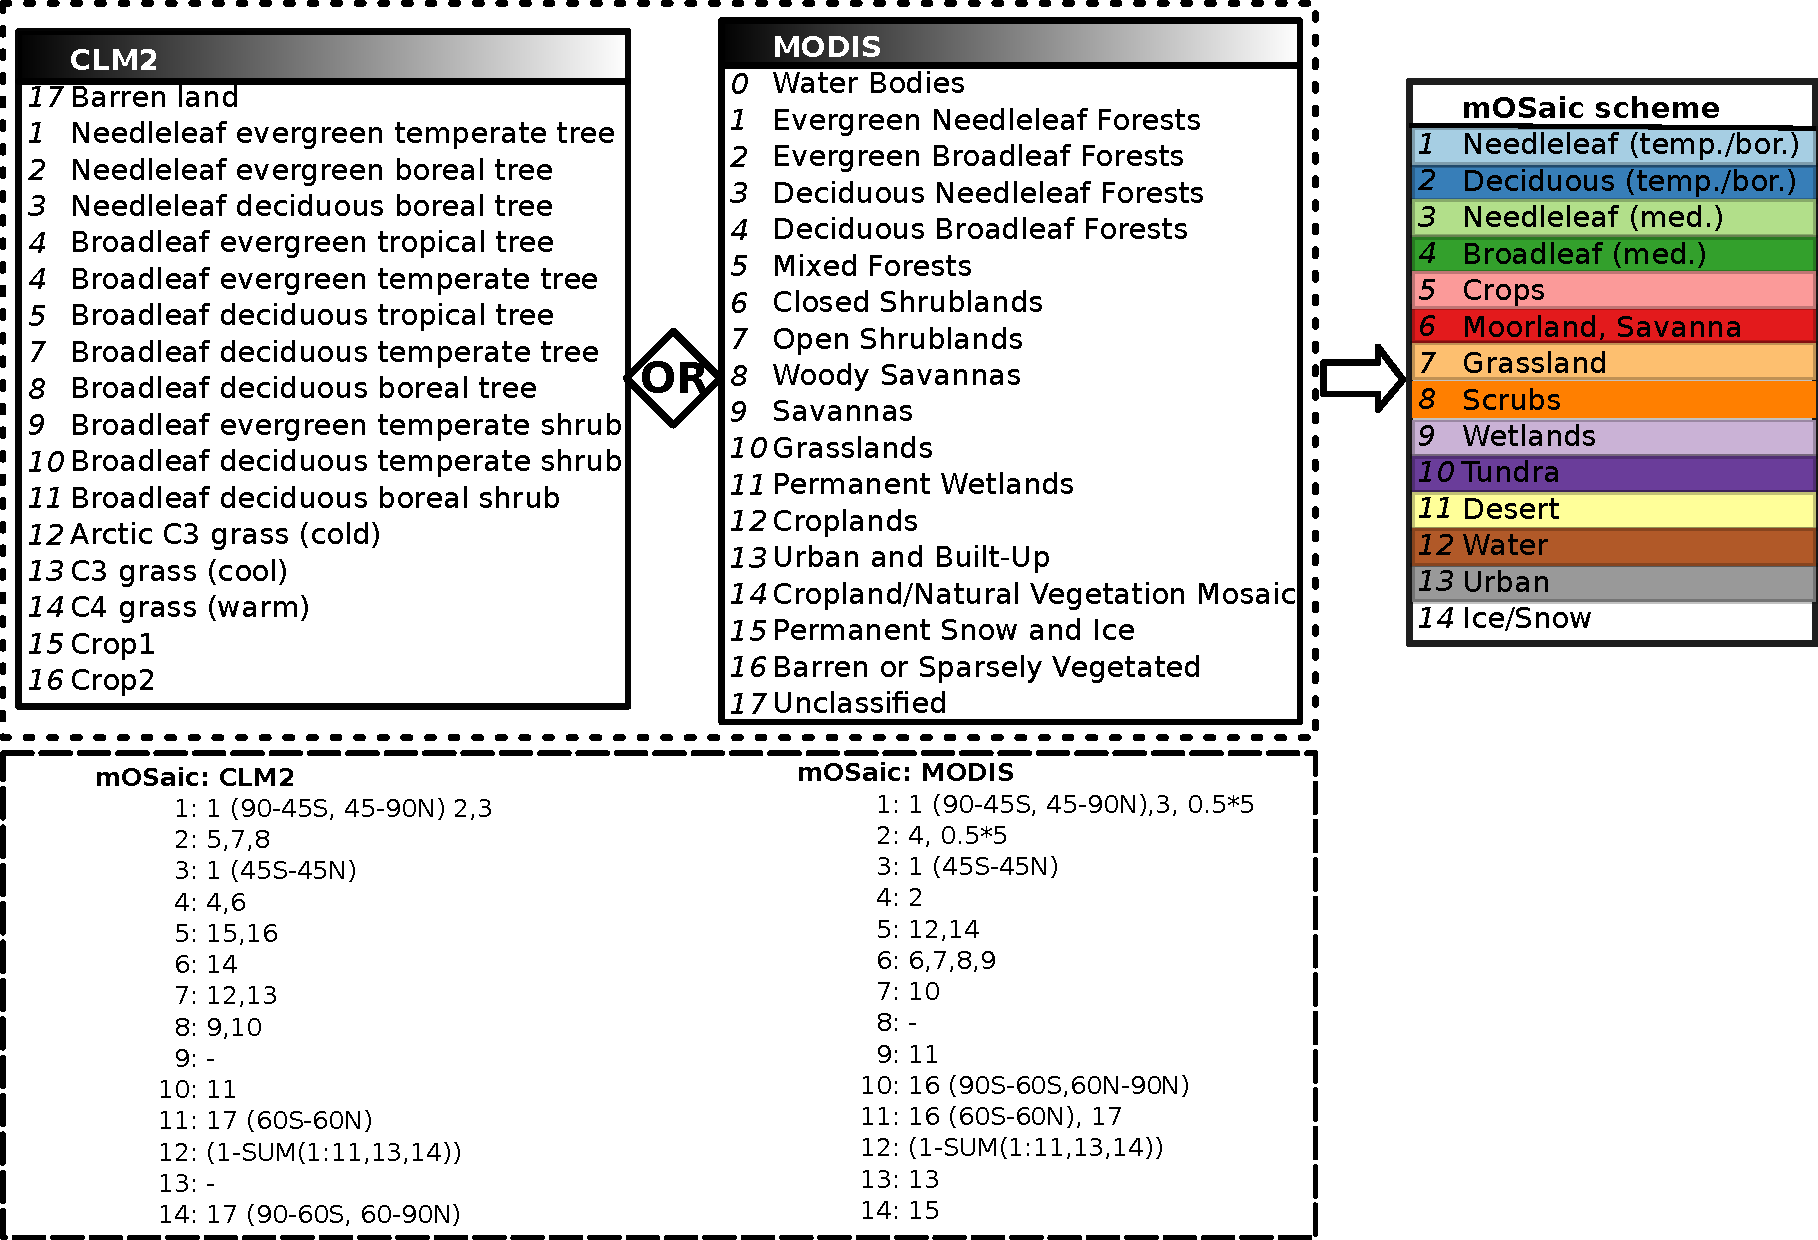
\includegraphics[width=12cm]{fig02}
  \caption{Mapping of land surface categories. Either land surface categories from ISLSCP2 product of MODIS \DIFdelbeginFL \DIFdelFL{/  }\DIFdelendFL \DIFaddbeginFL \DIFaddFL{or the }\DIFaddendFL Community Land Model (CLM)~2 can be chosen for mapping to the \DIFdelbeginFL \DIFdelFL{nine }\DIFdelendFL land surface types \DIFdelbeginFL \DIFdelFL{used }\DIFdelendFL \DIFaddbeginFL \DIFaddFL{we use }\DIFaddendFL in the \DIFdelbeginFL \DIFdelFL{EMAP }\DIFdelendFL \DIFaddbeginFL \DIFaddFL{mOSaic }\DIFaddendFL scheme. Water bodies \DIFdelbeginFL \DIFdelFL{and snow and ice categories }\DIFdelendFL of MODIS are actually not mapped. For both, MODIS and CLM~2 land surface categories, snow and ice cover is estimated from input meteorology, while water is defined as \DIFdelbeginFL \DIFdelFL{$1-\sum_{N=0}^{N_\text{max}} f_L(N)$}\DIFdelendFL \DIFaddbeginFL \DIFaddFL{$1-\sum_{k} f_L^k$}\DIFaddendFL . From MODIS category \emph{Barren or sparsely vegetated}, everything polward from $60\,\unit{^\circ}$ is defined as tundra, while everything equatorward is categorized as desert.}
  \label{fig:pft_mapping}
\end{figure*}
%
%%%%%%%%%%%%%%%%%%%%%%%%%%%%
\subsection{Pre-processing}
\label{subsec:pre-pro}
As mentioned in the previous section, there are two variables needed for computing the stomatal conductance which are not directly available from the meteorological input data. The greening season, as the time of the year in the mid and high latitudes when it is most likely for plants to grow, and the photosynthetic photon flux density, as the amount of light that plants need to photosynthesize. In the following, we present the necessary pre-processing of the variables. It is planed to implement an online computation of these variables into the Oslo~CTM3 later on.
%%%%%%%%%%%%%%%%%%%%%%%%%%%%
\subsubsection{Greening season}
\label{subsubsec:greening}
In Eqs.~(\ref{eq:non-stomata-cond}--\ref{eq:SAI}), \citet{ACP:Simpson2012} use prescribed start of growing season (SGS) and end of growing season (EGS) at $50\,\unit{^\circ N}$ ($d_\text{SGS}$, $d_\text{EGS}$) together with lapse rates ($\nabla d_\text{SGS}$, and $\nabla d_\text{EGS}$) to define phenology and dry deposition over agricultural areas. For the growing season of crops in the computation of non-stomatal conductances, we use also prescribed values (Table~\ref{tab:growing_season}), while for the stomatal conductances, as shown in Eq.~(\ref{eq:fphen}), we use the SGS and EGS derived parameters: day of greening season (GDAY), the time elapsed starting at the SGS, and the total length of the greening season (GLEN), the time span between EGS and SGS. Since the \DIFdelbegin \DIFdel{eurocentric EMEP }\DIFdelend parameterization of SGS and EGS \DIFaddbegin \DIFadd{in \mbox{%DIFAUXCMD
\citet{ACP:Simpson2012} }\hspace{0pt}%DIFAUXCMD
}\DIFaddend is not applicable in a global model, another latitude dependent parameterization is needed. First, we \DIFdelbegin \DIFdel{have }\DIFdelend used a parameterization \DIFdelbegin \DIFdel{as }\DIFdelend \DIFaddbegin \DIFadd{which was already }\DIFaddend implemented in the \DIFaddbegin \DIFadd{Oslo~CTM3 and which had been adopted from the }\DIFaddend Sparse Matrix Operational Kernel Emissions -- Biogenic Emission Inventory System (SMOKE-BEIS; \href{https://www.epa.gov/air-emissions-modeling/biogenic-emission-inventory-system-beis}{model webpage}). SMOKE-BEIS has fixed values for SGS and EGS for all regions but NH mid latitudes ($23\,\unit{^\circ} < \text{lat} < 65\,\unit{^\circ}$), where it uses lapse rates of $\nabla d_\text{SGS} = 4.5$ and $\nabla d_\text{EGS} = 3.3$. As this parameterization is optimized for North America, it does not work well in Europe, e.g., most of northern Scandinavia has no allocated vegetation period. \DIFaddbegin \DIFadd{This basically results in a suppression of canopy resistance in northern Scandinavia.}\DIFaddend \\ 

In agriculture, there are different empirical rules to estimate the SGS and EGS. The simplest assumption is that greening starts after $5$ consecutive days with a daily average temperature above $5\,\unit{^\circ C}$ and vice versa for EGS. Other estimates use growing degree days \citep{JC:Levis2004,PO:Fu2014}, include soil moisture \citep{GCB:Fu2014}, or rely on satellite observations. A comprehensive evaluation of different techniques is given by \citet{GCB:Anav2017}. \DIFaddbegin \DIFadd{Another solution would be the usage of a proper land surface model, e.g. LPJ-GUESS, CLM, but the integration of such into the Oslo~CTM3 is not planed at the moment.
}\DIFaddend 

Based on the empirical rule ($5\,\unit{^\circ C}$-days), we have pre-processed our meteorological input data offline. We added some additional criteria to prevent for \emph{false spring}: If, within these $5$ days, the average temperature drops below or rises above $5\,\unit{^\circ C}$, the counter is reset, respectively. First, we used the $5\,\unit{^\circ C}$-days criteria for $45\,\unit{^\circ} < \text{lat} < 85\,\unit{^\circ}$ in the NH, but extended it also to $35\,\unit{^\circ} < \text{lat} < 65\,\unit{^\circ}$ in the SH. In all other cases and where the $5\,\unit{^\circ C}$-days criteria fails, we still use the SMOKE-BEIS parameterization. The described algorithm written in python~2.7 has been included as Supplement~S\DIFdelbegin \DIFdel{.5}\DIFdelend \DIFaddbegin \DIFadd{.4}\DIFaddend . An example map of the computed GLEN using the $5\,\unit{^\circ C}$-days criteria in both hemispheres is shown in Fig.~\ref{fig:glen_2015_she}.
%
\begin{figure}[t]
  \includegraphics[width=8.3cm, clip, trim={0.cm 1.75cm 0.cm 1.75cm}]{fig03}
  \caption{Pre-processing of greening season from meteorological surface temperature fields. Shown is the total length of the greening season (GLEN) for the year 2005. The $5\,\unit{^\circ C}$-days criteria has been used in both hemispheres mid--high latitudes. Ocean has been shaded to indicate that greening season will only affect land.}
  \label{fig:glen_2015_she}
\end{figure}
%
%%%%%%%%%%%%%%%%%%%%%%%%%%%%
\subsubsection{Photosynthetic photon flux density}
From OpenIFS an accumulated surface PAR is available\DIFdelbegin \DIFdel{which is already integrated presumably over the spectrum }\DIFdelend \DIFaddbegin \DIFadd{. It is integrated both, spactrally (presumably }\DIFaddend $400-700\,\unit{nm}$\DIFdelbegin \DIFdel{. For this reason, it will be refered to as PPFD instead of PAR. This PPFD field has not been de-accumulated in the post-processing of the OpenIFS output and it is not feasible to redo all of the post-processing for this work. But for }\DIFdelend \DIFaddbegin \DIFadd{) and temporally. For }\DIFaddend practical use in Eq.~(\ref{eq:flight}), \DIFdelbegin \DIFdel{this field needs to be de-accumulated.
}\DIFdelend \DIFaddbegin \DIFadd{we de-accumulate this field with respect to time and refer to the result as PPFD.
}

\DIFaddend The main obstacle is that PAR has been accumulated since model start, so that the first field kept from the original OpenIFS simulation ($00\,\unit{UTC}$) is $12$ hours after model start ($12\,\unit{UTC}$ on the previous day). In other words, the first time step of each day in the Oslo~CTM3 has already accumulated PAR from $12\,\unit{UTC}$ on the previous day.
De-accumulation of times $03\,\unit{UTC}$ to $21\,\unit{UTC}$, simply means computing the difference
\begin{equation}
  \text{PPFD}(t_i) = \text{PAR}(t_{i+1})-\text{PAR}(t_i).
\end{equation}
For de-accumulation of the remaining \DIFdelbegin \DIFdel{timestep}\DIFdelend \DIFaddbegin \DIFadd{time step}\DIFaddend , the best choice is subtracting the difference between $21\,\unit{UTC}$ and $12\,\unit{UTC}$ of the previous day
%
\begin{equation}
  \text{PPFD}(t=00\,\unit{UTC}) = \text{PAR}(t=00\,\unit{UTC}) - \left[\text{PAR}(t=21\,\unit{UTC}-1\,\unit{day})-\text{PAR}(t=12\,\unit{UTC}-1\,\unit{day})\right]
\end{equation}
%
and limit the result to positive values only. An example PAR de-accumulation for January 2nd 2005 is shown in Supplement~S\DIFdelbegin \DIFdel{.6 }\DIFdelend \DIFaddbegin \DIFadd{.5 }\DIFaddend (Figs.~S5--S7).
The resulting PPFD fields are still accumulated over a time period of $3$ hours and should be divided by $3$. A \href{https://confluence.ecmwf.int/display/CKB/ERA-Interim\%3A+surface+photosynthetically+active+radiation+\%28surface+PAR\%29+values+are+too+low}{known issue} in the OpenIFS (cycles $\le$ c41r2) causes surface PAR values to be about $30\,\unit{\%}$ below observations. To counter this, we decided to refrain from the division at this stage, but need to bear this in mind for later OpenIFS cycles.
\DIFaddbegin 

\DIFaddend %%%%%%%%%%%%%%%%%%%%%%%%%%%%      
\section{Evaluation}
\label{sec:eval}
In this section, we present results from a manifold of Oslo~CTM3 model integrations testing different parameters of the \DIFdelbegin \DIFdel{EMEP }\DIFdelend \DIFaddbegin \DIFadd{mOSaic }\DIFaddend scheme. We focus on changes in ozone \DIFdelbegin \DIFdel{related to the stomatal conductance parameterization, e.g., }\DIFdelend total dry deposition $\sum\chem{O_3^\text{DD}}$, dry deposition velocities $v^\chem{O_3}_\text{DD}$, \DIFdelbegin \DIFdel{and surface concentration $[\chem{O_3}](z_0)$ or surface burden $\chem{O_3}(z_0)$ in units of }%DIFDELCMD < \unit{kg}%%%
\DIFdel{, respectively}\DIFdelend \DIFaddbegin \DIFadd{concentrations in the lowermost model level $[\chem{O_3}](p_0)$, and tropospheric burden $\sum_\text{trop}\chem{O_3}$}\DIFaddend . We evaluate our results with respect to the multi-model comparison of ozone dry deposition by \citet{ACP:Hardacre2015} (Section~\ref{subsec:model})\DIFaddbegin \DIFadd{, the MACC-reanalysis (Section~\ref{subsec:macc}), }\DIFaddend and observations (Section~\ref{subsec:obs}). The Oslo~CTM3 is driven by meteorological input fields from \href{https://www.ecmwf.int/en/forecasts/documentation-and-support/evolution-ifs/cycle-38r1-summary-changes}{ECMWF -- OpenIFS cy38r1}. CEDS historical emission inventory is used for anthropogenic emissions, while biomass burning is covered in daily resolution by NASA's Global Fire Emissions Database, Version4 (GFEDv4). Biogenic emissions are taken from MEGAN-MACC output \citep{ACP:Sindelarova2014}\DIFaddbegin \DIFadd{, while emissions from soil and wetlands are computed by MEGAN. Resultant $\mathrm{NO_x}$ emissions are up-scaled to match Global Emissions InitiAtive (GEIA) inventory. For oceanic emissions of }\chem{CO}\DIFadd{, we use predefined global fields from POET \mbox{%DIFAUXCMD
\citep{POET}}\hspace{0pt}%DIFAUXCMD
. Emissions of }\chem{CH_4} \DIFadd{are taken from the EU project (EU GOCE 037048) Hydrogen, Methane and Nitrous oxide: Trend variability, budgets and interactions with the biosphere (HYMN) for the year 2003 and scaled to oceanic amounts of $\mathrm{CH_4}$ from NASA}\DIFaddend . In the following (Section~\ref{subsec:sens}), we will present the various model sensitivity studies.
%%%%%%%%%%%%%%%%%%%%%%%%%%%%
\subsection{Sensitivity studies}
\label{subsec:sens}
Due to significant differences between the \DIFdelbegin \DIFdel{EMEP }\DIFdelend \DIFaddbegin \DIFadd{mOSaic }\DIFaddend scheme and the previous Wesely scheme with respect to implementation, it is not possible to fully disentangle and trace back every \DIFaddbegin \DIFadd{single }\DIFaddend difference in results to a respective change. Therefore, we conducted \DIFdelbegin \DIFdel{in total nine sensitivity studies that mainly assess }\DIFdelend \DIFaddbegin \DIFadd{one reference simulation denoted as }\emph{\DIFadd{mOSaic}} \DIFadd{and in total seven sensitivity studies to probe }\DIFaddend the parameter space \DIFdelbegin \DIFdel{of the stomatal conductance within the EMEP scheme}\DIFdelend \DIFaddbegin \DIFadd{for stomatal conductance (}\emph{\DIFadd{mOSaic\_offLight}}\DIFadd{, }\emph{\DIFadd{mOSaic\_offPhen}}\DIFadd{, and }\emph{\DIFadd{mOSaic\_SWVL1}}\DIFadd{), ozone surface resistance $R^\chem{O_3}$ (}\emph{\DIFadd{mOSaic\_ice}}\DIFadd{, }\emph{\DIFadd{mOSaic\_desert}}\DIFadd{, and }\emph{\DIFadd{mOSaic\_hough}}\DIFadd{), and emissions (}\emph{\DIFadd{mOSaic\_emis2014}}\DIFadd{)}\DIFaddend . A reference simulation featuring the \DIFaddbegin \DIFadd{Oslo~CTM3 }\DIFaddend Wesely scheme has been conducted and will be referred to as \emph{Wesely\_type}, indicating that other implementations of the original work by \citet{AE:Wesely1989} may exist in other models.
\DIFaddbegin \DIFadd{All model experiments discussed in the following are summarized in Table~\ref{tab:simsum}. An }\emph{\DIFadd{x}} \DIFadd{therein denotes that the model was run exactly in the configuration and with parameters as has been described in Section~\ref{sec:model_des}.
}\DIFaddend For all model integrations, the meteorological reference year is 2005. This choice \DIFdelbegin \DIFdel{only affects the }\DIFdelend \DIFaddbegin \DIFadd{affects the direct }\DIFaddend comparison with data and \DIFdelbegin \DIFdel{multi-model }\DIFdelend studies that either \DIFdelbegin \DIFdel{perform analysis }\DIFdelend \DIFaddbegin \DIFadd{show results based }\DIFaddend on decadal averages or differing years\DIFdelbegin \DIFdel{. After finishing the work on the integration of the EMEP parameterization and initial testing, }\emph{\DIFdel{EMEP\_full}} %DIFAUXCMD
\DIFdel{is the baseline simulation for the sensitivity studies, }\emph{\DIFdel{EMEP\_offLight}} %DIFAUXCMD
\DIFdel{and }\emph{\DIFdel{EMEP\_offPhen}}%DIFAUXCMD
\DIFdelend \DIFaddbegin \DIFadd{, because non-linearities in ozone formation and destruction make ozone concentrations sensitive to both, differences in local concentration of precursors and meteorological conditions \mbox{%DIFAUXCMD
\citep{JGR:Jin2013}}\hspace{0pt}%DIFAUXCMD
.
}

\DIFadd{First, we have a closer look at the influence of certain parameters on the stomatal conductance}\DIFaddend . As indicated by the names, \DIFdelbegin \DIFdel{these scenarios are extreme cases, }\DIFdelend \DIFaddbegin \emph{\DIFadd{mOSaic\_offLight}} \DIFadd{and }\emph{\DIFadd{mOSaic\_offPhen}} \DIFadd{are rather extreme scenarios completely switching off the sensitivity to light and phenology in Eq.~(\ref{eq:stomatal}) by }\DIFaddend setting $f_\text{light}$ and $f_\text{phen}$ to \DIFaddbegin \DIFadd{a fixed value of }\DIFaddend 1, respectively. \DIFdelbegin \DIFdel{During analysis of the results, we found, that the SMOKE-BEIS parameterization of the greening season did not extend to the boreal and subarctic regions. Especially in Europe, this basically results in a suppression of canopy resistance in northern Scandinavia. The following sensitivity study therefore comprises two different versions of pre-processed greening season (refer to Section~\ref{subsec:pre-pro} for details) : Mid and high latitudes in the northern hemisphere only (}\emph{\DIFdel{EMEP\_ppgs}}%DIFAUXCMD
\DIFdel{) and for both, northern and southern hemisphere mid and high latitudes (}\emph{\DIFdel{EMEP\_ppgssh}}%DIFAUXCMD
\DIFdel{). 
Building on the latter}\DIFdelend \DIFaddbegin \DIFadd{Because of the underlying research project's focus on arctic and alpine ecosystems, where water might only be available from upper soil layers, an experiment was conducted using the uppermost soil water level (SWVL1) in the implementation of $f_\text{SW}$. 
After this}\DIFaddend , we want to confirm the importance of \DIFdelbegin \DIFdel{the $v^\chem{O_3}_\text{ice/snow}$ update \mbox{%DIFAUXCMD
\citep{ACP:Helmig2007} }\hspace{0pt}%DIFAUXCMD
in the Subarctic and Arctics, within the framework of the Oslo~CTM3 (}\DIFdelend \DIFaddbegin \DIFadd{choice of $R^\chem{O_3}$ for different land surface types. We conducted three experiments looking at a $R^\chem{O_3}_\text{ice/snow}$ update \mbox{%DIFAUXCMD
\citep{ACP:Helmig2007} }\hspace{0pt}%DIFAUXCMD
(}\emph{\DIFadd{mOSaic\_ice}}\DIFadd{), observed $R^\chem{O_3}_\text{desert}$ \mbox{%DIFAUXCMD
\citep{AE:Gusten1995} }\hspace{0pt}%DIFAUXCMD
(}\DIFaddend \emph{\DIFdelbegin \DIFdel{EMEP\_ppgssh}\DIFdelend \DIFaddbegin \DIFadd{mOSaic}\DIFaddend \_\DIFdelbegin \DIFdel{ice}\DIFdelend \DIFaddbegin \DIFadd{desert}\DIFaddend })\DIFdelbegin \DIFdel{. Accidentally, we have used }\DIFdelend \DIFaddbegin \DIFadd{, and an approximation of $R^\chem{O_3}$ originally used in }\emph{\DIFadd{Wesely\_type}} \DIFadd{\mbox{%DIFAUXCMD
\citep{AE:Wesely1989, JGR:Hough1991}}\hspace{0pt}%DIFAUXCMD
.
Finally, we run a simulation with }\DIFaddend emissions for the year 2014 instead of \DIFdelbegin \DIFdel{2005. Though, we take this as opportunity to assess the impact on ozone regarding differing emissions (}\emph{\DIFdel{EMEP\_ppgs\_2005}}%DIFAUXCMD
\DIFdel{). As mentioned previously, the simulations were initially conducted with the uppermost soil water level (SWVL1) in the implementation of $f_\text{SW}$. A final sensitivity study was conducted changing to soil water level at depths deeper than $1\,\unit{m}$ (}\emph{\DIFdel{EMEP\_SWVL4}}%DIFAUXCMD
\DIFdel{).
All simulations discussed in this section are summarized in Table~\ref{tab:simsum}. An x in the table denotes that the model was run exactly in the configuration as has been described in Section~\ref{sec:model_des}}\DIFdelend \DIFaddbegin \DIFadd{2005 (}\emph{\DIFadd{EMEP\_emis2014}}\DIFadd{) to characterize the general influence of differing emissions on ozone}\DIFaddend .  

\begin{table*}[t]
  \caption{Summary of specifications of all simulations discussed in this section. For simplicity, only the tested parameters are listed. An x denotes that the model was run exactly in the configuration as has been described in Section~\ref{sec:model_des}.}
  \begin{tabular}{lccccccccc}
    \tophline
    ...\\
    \bottomhline
  \end{tabular}
  \label{tab:simsum}
  %DIF < \belowtable{} % Table Footnotes
\DIFaddbeginFL \belowtable{$^\dagger\,R^\chem{O_3}_\text{ice/snow}=10000\,\unit{s\,m^{-1}}$; $^*\,R^\chem{O_3}_\text{desert}=800\,\unit{s\,m^{-1}}$; $^\star\,$For adapted values see Supplement~S.6} %DIF >  Table Footnotes
\DIFaddendFL \end{table*}
%
\begin{figure}[t]
  \includegraphics[width=8.3cm]{fig04}
  \caption{Relative difference between \DIFdelbeginFL \DIFdelFL{the sensitivity simulation }\emph{\DIFdelFL{EMEP\_ppgsssh}} %DIFAUXCMD
\DIFdelendFL \DIFaddbeginFL \DIFaddFL{reference simulations }\emph{\DIFaddFL{mOSaic}} \DIFaddendFL and the \emph{Wesely\_type} \DIFdelbeginFL \DIFdelFL{in }\DIFdelendFL \DIFaddbeginFL \DIFaddFL{with respect to }\DIFaddendFL (a) \DIFdelbeginFL \DIFdelFL{total surface }\DIFdelendFL \DIFaddbeginFL \DIFaddFL{average }\DIFaddendFL ozone \DIFaddbeginFL \DIFaddFL{burden in the lowermost model level}\DIFaddendFL ; (b) average ozone dry deposition velocity; (c) total amount of ozone removed from the atmosphere by dry deposition.}
  \label{fig:diff_maps}
\end{figure}
%
In Fig.~\ref{fig:diff_maps}, we show the average relative difference between \emph{\DIFdelbegin \DIFdel{EMEP\_ppgsssh}\DIFdelend \DIFaddbegin \DIFadd{mOSaic}\DIFaddend } and \emph{Wesely\_type} on global maps by means of \DIFdelbegin \DIFdel{surface ozone burden }\DIFdelend \DIFaddbegin \DIFadd{ozone burden in the lowermost model level}\DIFaddend , dry deposition velocity and total ozone dry deposition. \DIFdelbegin \DIFdel{Surface ozone }\DIFdelend \DIFaddbegin \DIFadd{The ozone burden }\DIFaddend increases globally except for \DIFaddbegin \DIFadd{some }\DIFaddend regions covered by tropical forest. Especially in desert regions in Africa\DIFaddbegin \DIFadd{, America, }\DIFaddend and Asia, \DIFdelbegin \DIFdel{surface ozone increases by up to }\DIFdelend \DIFaddbegin \DIFadd{ozone burden increases by more then }\DIFaddend $100\,\unit{\%}$. Consistently, dry deposition velocities decrease globally by the same order of magnitude in these regions, while they increase over tropical forest. With respect to total dry deposition, the picture is a bit less clear. We find a decrease of total dry deposition of ozone in desert regions and ocean covered areas and an increase in regions covered by tropical forest, while at mid and high latitudes in both hemispheres only small changes are visible. A possible explanation to this divergence especially in desert regions is the difference between the prescribed \DIFdelbegin \DIFdel{dry deposition velocities }\DIFdelend \DIFaddbegin \DIFadd{surface resistances $R^\chem{O_3}$ }\DIFaddend in the Wesely scheme in comparison to those used in \DIFdelbegin \DIFdel{the EMEP scheme. We cover this in more detail in the following section}\DIFdelend \DIFaddbegin \emph{\DIFadd{mOSaic}}\DIFadd{. We come back to this in the following sections}\DIFaddend .

%%%%%%%%%%%%%%%%%%%%%%%%%%%%
\subsection{Comparison with modeling results}
\label{subsec:model}
%
In \DIFdelbegin \DIFdel{our evaluation of results}\DIFdelend \DIFaddbegin \DIFadd{the evaluation of our model}\DIFaddend , we closely follow suggestions by \citet{ACP:Hardacre2015}. For the purpose of comparison with the multi-model mean of the therein participating Task Force on Hemispheric Transport of Air Pollution (TF~HTAP) models, we also have re-gridded our data to a horizontal resolution of $3^\circ\times 3^\circ$. In Section~\ref{subsubsec:zonal}, we look at zonal distributions of \DIFdelbegin \DIFdel{$[\chem{O_3}](z_0)$}\DIFdelend \DIFaddbegin \DIFadd{$[\chem{O_3}](p_0)$}\DIFaddend , $v^\chem{O_3}_\text{DD}$, and $\sum\chem{O_3^\text{DD}}$ for all our sensitivity simulations and study seasonal cycles of hemispheric ozone as well as for nine land surface types \DIFdelbegin \DIFdel{which have been retrospectively separated }\DIFdelend (Section~\ref{subsubsec:seasons}). From this, we estimate the total annual ozone dry deposition onto ocean, ice, and land surfaces and compare also with results from \citet{ACP:Luhar2017}.

\DIFdelbegin \DIFdel{As dry }\DIFdelend \DIFaddbegin \DIFadd{Dry }\DIFaddend deposition velocities are \DIFdelbegin \DIFdel{not directly available from the model output, monthly average }\DIFdelend \DIFaddbegin \DIFadd{directly available only for the new model version. For }\emph{\DIFadd{Wesely\_type}}\DIFadd{, monthly averaged }\DIFaddend dry deposition velocities $v^\chem{O_3}_\text{DD}$ \DIFdelbegin \DIFdel{have been reconstructed }\DIFdelend \DIFaddbegin \DIFadd{had to be retrospectively estimated }\DIFaddend from the ratio between the total ozone dry deposition \DIFdelbegin \DIFdel{$\sum \chem{O_3^\text{DD}}(z_0)$ }\DIFdelend \DIFaddbegin \DIFadd{$\sum \chem{O_3^\text{DD}}(p_0)$ }\DIFaddend and monthly averaged \DIFdelbegin \DIFdel{surface ozone amount $\chem{O_3}(z_0)$ 
}\DIFdelend \DIFaddbegin \DIFadd{ozone amount in the lowermost model level $\chem{O_3}(p_0)$ 
}\DIFaddend \begin{equation}
  v^\chem{O_3}_\text{DD} = \DIFdelbegin \DIFdel{\frac{\sum \chem{O_3^\text{DD}}(z_0)}{\chem{O_3}(z_0)}}\DIFdelend \DIFaddbegin \DIFadd{\frac{\sum \chem{O_3^\text{DD}}(p_0)}{\chem{O_3}(p_0)}}\DIFaddend \cdot c_\text{month}.
  \DIFaddbegin \label{eq:retro_vdd}
\DIFaddend \end{equation}
Herein, $c_\text{month} = \frac{\Delta h_\text{month}}{s_\text{month}}$, with the monthly average height of the lowermost model level in each gridbox $\Delta h_\text{month}$ and the respective number of seconds in a month $s_\text{month}$. \DIFaddbegin \DIFadd{In case of }\emph{\DIFadd{mOSaic}}\DIFadd{, resulting values for $v^\chem{O_3}_\text{DD}$ from Eq.~(\ref{eq:retro_vdd}) are compatible with the values which are directly ailable from model output.
}\DIFaddend %
\subsubsection{Zonal distribution}
\label{subsubsec:zonal}
%
The annual zonal average with respect to surface ozone concentration (Fig.~\ref{fig:mmm_drydep}a\DIFaddbegin \DIFadd{) }\DIFaddend displays on average, in consistency with Fig.~\ref{fig:diff_maps}a, a global increase of surface ozone concentrations by \DIFdelbegin \DIFdel{up to $10\,\unit{ppb}$ when applying the EMEP scheme compared to the Wesely scheme}\DIFdelend \DIFaddbegin \DIFadd{$6\,\unit{ppb}$ comparing }\emph{\DIFadd{mOSaic}} \DIFadd{to }\emph{\DIFadd{Wesely\_type}}\DIFaddend . This increase is largest in the zonal band $(25-50)\,\unit{^\circ N}$ which contains the major deserts. In the deep tropics ($5\,\unit{^\circ S}-5\,\unit{^\circ N}$), the increase is smallest (\DIFdelbegin \DIFdel{$\Delta[\chem{O_3}]\leq 5\,\unit{ppb}$}\DIFdelend \DIFaddbegin \DIFadd{$\mathcal{O}(5\,\unit{ppb})$}\DIFaddend ). We find that the \DIFdelbegin \DIFdel{EMEP }\DIFdelend \DIFaddbegin \DIFadd{mOSaic }\DIFaddend scheme further intensifies the strong asymmetry between northern and southern hemisphere as a consequence of the distribution of the continental land masses and vegetation thereon. Among the sensitivity studies \DIFaddbegin \DIFadd{focusing on the stomatal conductance}\DIFaddend , there is only a low absolute variance. \DIFdelbegin \DIFdel{Most remarkable, but expected due to the much smaller prescribed dry deposition velocity over ice and snow, }\emph{\DIFdel{EMEP\_ppgssh\_ice}} %DIFAUXCMD
\DIFdel{displays almost a doubling of surface ozone in the high Arctics compared to }\emph{\DIFdel{Wesely\_type}} %DIFAUXCMD
\DIFdel{but affects ozone concentrations down to latitudes at about $50\,\unit{^\circ}$ in both hemispheres. Neglecting any dependence on solar radiation }\DIFdelend \DIFaddbegin \DIFadd{Neglecting the dependence on light }\DIFaddend in the stomatal conductance formulation (\emph{\DIFdelbegin \DIFdel{EMEP}\DIFdelend \DIFaddbegin \DIFadd{mOSaic}\DIFaddend \_offLight}) -- or in other words allowing photosynthesis 24/7 -- \DIFdelbegin \DIFdel{generally }\DIFdelend decreases the ozone concentration by \DIFdelbegin \DIFdel{about $2\,\unit{ppb}$}\DIFdelend \DIFaddbegin \DIFadd{$1-2\,\unit{ppb}$ in the tropics and NH mid latitudes}\DIFaddend , while choosing soil water at \DIFdelbegin \DIFdel{deeper levels than the surface layer (}\DIFdelend \DIFaddbegin \DIFadd{shallower depths (}\DIFaddend \emph{\DIFdelbegin \DIFdel{EMEP}\DIFdelend \DIFaddbegin \DIFadd{mOSaic}\DIFaddend \_\DIFdelbegin \DIFdel{SWVL4}\DIFdelend \DIFaddbegin \DIFadd{SWVL1}\DIFaddend }) increases \DIFdelbegin \DIFdel{$[\chem{O_3}](z_0)$ slightly}\DIFdelend \DIFaddbegin \DIFadd{$[\chem{O_3}]$ insignificantly}\DIFaddend . Rather surprisingly, switching off the phenology completely (\emph{\DIFdelbegin \DIFdel{EMEP}\DIFdelend \DIFaddbegin \DIFadd{mOSaic}\DIFaddend \_offPhen}) \DIFdelbegin \DIFdel{, amounts }\DIFdelend \DIFaddbegin \DIFadd{amounts on average }\DIFaddend only to small difference (\DIFdelbegin \DIFdel{at most $3.5\,\unit{\%}$ increase in the deep tropics) . Switching from the SMOKE-BEIS parameterization to the pre-processed greening season (}\emph{\DIFdel{EMEP\_ppgs}} %DIFAUXCMD
\DIFdel{compared to }\emph{\DIFdel{EMEP\_full}}%DIFAUXCMD
\DIFdel{) , surface ozone increases on average }\DIFdelend \DIFaddbegin \DIFadd{$\mathcal{O}(<1\,\unit{ppb})$). Most remarkable, but expected due to the much smaller prescribed dry deposition velocity over ice and snow, }\emph{\DIFadd{mOSaic\_ice}} \DIFadd{displays a doubling of surface ozone in the high Arctics compared to }\emph{\DIFadd{Wesely\_type}} \DIFadd{($\mathcal{O}(20\,\unit{ppb})$) but affects ozone concentrations down to latitudes at about $50\,\unit{^\circ}$ in both hemispheres. Reducing $R^\chem{O_3}_\text{desert}$ }\DIFaddend by \DIFdelbegin \DIFdel{$6\,\unit{\%}$ between $(54-70)\,\unit{^\circ N}$}\DIFdelend \DIFaddbegin \DIFadd{$60\,\unit{\%}$ (}\emph{\DIFadd{mOSaic\_desert}}\DIFadd{) a reduction in the order of $1\,\unit{ppb}$ is found mainly limited to the NH. The largest impact on ozone concentrations ($\mathcal{O}(2-5\,\unit{ppb})$) is found for the experiment }\emph{\DIFadd{mOSaic\_hough}} \DIFadd{which is closest to }\emph{\DIFadd{Wesely\_type}}\DIFadd{, since we used on average the same $R^\chem{O_3}$ (see Supplement~S.6)}\DIFaddend . The scenario of differing emissions (2005 in comparison to 2014 or more specifically \emph{\DIFdelbegin \DIFdel{EMEP\_ppgs\_2005}\DIFdelend \DIFaddbegin \DIFadd{mOSaic}\DIFaddend } compared to \emph{\DIFdelbegin \DIFdel{EMEP}\DIFdelend \DIFaddbegin \DIFadd{mOSaic}\DIFaddend \_\DIFdelbegin \DIFdel{ppgs}\DIFdelend \DIFaddbegin \DIFadd{emis2014}\DIFaddend }), yields higher ozone concentrations in the northern hemisphere in 2005 in accordance to a reduction in sulfur and \chem{NO_x} emissions in south east Asia in later years. An opposite tendency is seen for latitudes south of $30\,\unit{^\circ N}$, \DIFdelbegin \DIFdel{probably owing to the industrial development of countries in these regions}\DIFdelend \DIFaddbegin \DIFadd{where an increase in ozone precursors is seen in CEDS}\DIFaddend . 

The $v^\chem{O_3}_\text{DD}$ are shown in Fig.~\ref{fig:mmm_drydep}b. The dry deposition velocities in the \DIFdelbegin \DIFdel{EMEP scheme are on average $43\,\unit{\%}$ lower than in }\DIFdelend \DIFaddbegin \DIFadd{mOSaic scheme are well below }\DIFaddend the Wesely scheme \DIFaddbegin \DIFadd{and in remarkable agreement with the results shown by \mbox{%DIFAUXCMD
\citet{ACP:Hardacre2015}}\hspace{0pt}%DIFAUXCMD
}\DIFaddend . In the Arctics, except for \emph{\DIFdelbegin \DIFdel{EMEP\_ppgssh}\DIFdelend \DIFaddbegin \DIFadd{mOSaic}\DIFaddend \_ice}, all \DIFdelbegin \DIFdel{realizations of the EMEP scheme are constantly }\DIFdelend \DIFaddbegin \DIFadd{model experiments are slightly }\DIFaddend above the multi-model-mean. This indicates, that with respect to \DIFaddbegin \DIFadd{the }\DIFaddend other models, the \DIFdelbegin \DIFdel{updated dry deposition velocity }\DIFdelend \DIFaddbegin \DIFadd{\mbox{%DIFAUXCMD
\citet{ACP:Helmig2007} }\hspace{0pt}%DIFAUXCMD
surface resistance }\DIFaddend above ice and snow should be considered as new standard for the Oslo~CTM3. This may, however, lead to an overcompensation of the current \DIFaddbegin \DIFadd{arctic }\DIFaddend low-bias in surface ozone in the Oslo~CTM3 \DIFaddbegin \DIFadd{and needs further evaluation}\DIFaddend . The dry deposition velocities are of course independent of the emission scenario, but display a strong \DIFdelbegin \DIFdel{dependence }\DIFdelend \DIFaddbegin \DIFadd{sensitivity }\DIFaddend on $f_\text{light}$\DIFdelbegin \DIFdel{and $f_\text{phen}$. The closer to $1$ these factors are the higher the dry deposition velocities become (compare }\emph{\DIFdel{EMEP\_offLight}}%DIFAUXCMD
\DIFdel{, }\emph{\DIFdel{EMEP\_offPhen}}%DIFAUXCMD
\DIFdel{, and }\emph{\DIFdel{EMEP\_ppgssh}}%DIFAUXCMD
\DIFdel{). That highlights the importance of a proper PAR from meteorological input in CTMs or radiative transfer in PAR in global climate models (GCMs) and a proper choice of phenology for canopy conductance computation. Albeit, the total numbers are smaller, the }\DIFdelend \DIFaddbegin \DIFadd{, $f_\text{phen}$, and especially on the choice of $R^\chem{O_3}$. The }\DIFaddend shape of the normalized zonal average dry deposition velocities of the \DIFdelbegin \DIFdel{EMEP scheme and the multi-model-mean are similar }\DIFdelend \DIFaddbegin \DIFadd{mOSaic scheme are more similar to the multi-model-mean than to }\emph{\DIFadd{Wesely\_type}} \DIFaddend (Supplement~S.7: Fig.~S8). The biggest exceptions are the zonal bands $(50-70)\,\unit{^\circ S}$ \DIFdelbegin \DIFdel{, which is }\DIFdelend \DIFaddbegin \DIFadd{(}\DIFaddend almost entirely covered by ocean\DIFaddbegin \DIFadd{)}\DIFaddend , $(12-30)\,\unit{^\circ S}$ \DIFdelbegin \DIFdel{, which coincides }\DIFdelend \DIFaddbegin \DIFadd{(coinciding }\DIFaddend with the location of Australia and its desert regions\DIFaddbegin \DIFadd{)}\DIFaddend , as well as its counterpart in the northern hemisphere $(12-30)\,\unit{^\circ N}$.
\DIFdelbegin \DIFdel{However, it is not clear whether diverging dry deposition velocities over ocean or deserts have the larger impact.
}\DIFdelend 

The annual total ozone dry deposition is shown in Fig.~\ref{fig:mmm_drydep}c. In accordance to the previously described features, we observe a reduction of the global total ozone dry deposition in all sensitivity studies\DIFdelbegin \DIFdel{to almost }\DIFdelend \DIFaddbegin \DIFadd{. In the most extreme case (NH subtropics and mid latitudes), the total ozone dry deposition drops to }\DIFaddend one-half of the amount given by \emph{Wesely\_type}. The occurrence of this reduction in the zonal bands, where the major deserts are located, points to a \DIFdelbegin \DIFdel{change }\DIFdelend \DIFaddbegin \DIFadd{substantial difference }\DIFaddend in $v_\text{desert}^\chem{O_3}$. Consulting the parameter file used in the Wesely scheme, we indeed find $v_\text{desert}^\chem{O_3} \equiv v_\text{tundra}^\chem{O_3} = 0.26\,\unit{cm\,s^{-1}}$ \citep{JGR:Hough1991}, while in the \DIFdelbegin \DIFdel{EMEP }\DIFdelend \DIFaddbegin \DIFadd{mOSaic }\DIFaddend scheme $v_\text{desert}^\chem{O_3}=0.05\,\unit{cm\,s^{-1}}$ and $v^\chem{O_3}_\text{tundra} = 0.24\,\unit{cm\,s^{-1}}$, respectively. Similarly, dry deposition velocities over ice and snow and ocean have been even higher in the Wesely scheme ($v_\text{ice/snow}^\chem{O_3}\equiv v_\text{water}^\chem{O_3}=0.07\,\unit{cm\,s^{-1}}$) than in the original \DIFdelbegin \DIFdel{EMEP scheme ($v_\text{ice/snow}^\chem{O_3}\equiv v_\text{water}^\chem{O_3}=0.05\,\unit{cm\,s^{-1}}$)}\DIFdelend \DIFaddbegin \DIFadd{parameter set \mbox{%DIFAUXCMD
\citep[$v_\text{ice/snow}^\chem{O_3}\equiv v_\text{water}^\chem{O_3}=0.05\,\unit{cm\,s^{-1}}$,][]{ACP:Simpson2012}}\hspace{0pt}%DIFAUXCMD
}\DIFaddend . These differences in \DIFdelbegin \DIFdel{baseline dry deposition velocities }\DIFdelend \DIFaddbegin \DIFadd{surface resistances }\DIFaddend over huge parts of the unvegetated surface of the Earth \DIFdelbegin \DIFdel{amount to }\DIFdelend \DIFaddbegin \DIFadd{accounts for }\DIFaddend most of the \DIFdelbegin \DIFdel{quantitative }\DIFdelend \DIFaddbegin \DIFadd{qualitative }\DIFaddend difference between the Wesely and the \DIFdelbegin \DIFdel{EMEP scheme}\DIFdelend \DIFaddbegin \DIFadd{mOSaic scheme, but does not explain the quantitative difference (compare }\emph{\DIFadd{mOSaic\_hough}}\DIFadd{)}\DIFaddend . We further elaborate on this in the following \DIFdelbegin \DIFdel{section }\DIFdelend (Section~\ref{subsubsec:seasons}).

There seems to be a discrepancy between the Oslo~CTM3 response and the multi-model-mean, since the Wesely scheme is similar to the multi-model-mean with respect to total annual ozone dry deposition, while the \DIFdelbegin \DIFdel{reconstructed }\DIFdelend $v_\text{DD}^\chem{O_3}$ of the \DIFdelbegin \DIFdel{EMEP }\DIFdelend \DIFaddbegin \DIFadd{mOSaic }\DIFaddend scheme match better. This could be a sign of differences in photo-chemistry and transport (e.g. convective, advective, STE) between the Oslo~CTM3 and the average TF~HTAP model, but without comparing to the actual \DIFdelbegin \DIFdel{$[\chem{O_3}(z_0)]$ }\DIFdelend \DIFaddbegin \DIFadd{$[\chem{O_3}]$ }\DIFaddend of the TF~HTAP models that participated in the model intercomparison, we cannot elaborate on this any further. \DIFaddbegin \DIFadd{This may also hint to issues in the Oslo~CTM3 photo-chemistry, which may have a too high ozone production, or the actual removal of ozone from the atmosphere, which might have been adjusted to the less physical dry deposition velocities in the past, but this is subject to further investigations.
}\DIFaddend 

\begin{figure}[t]
  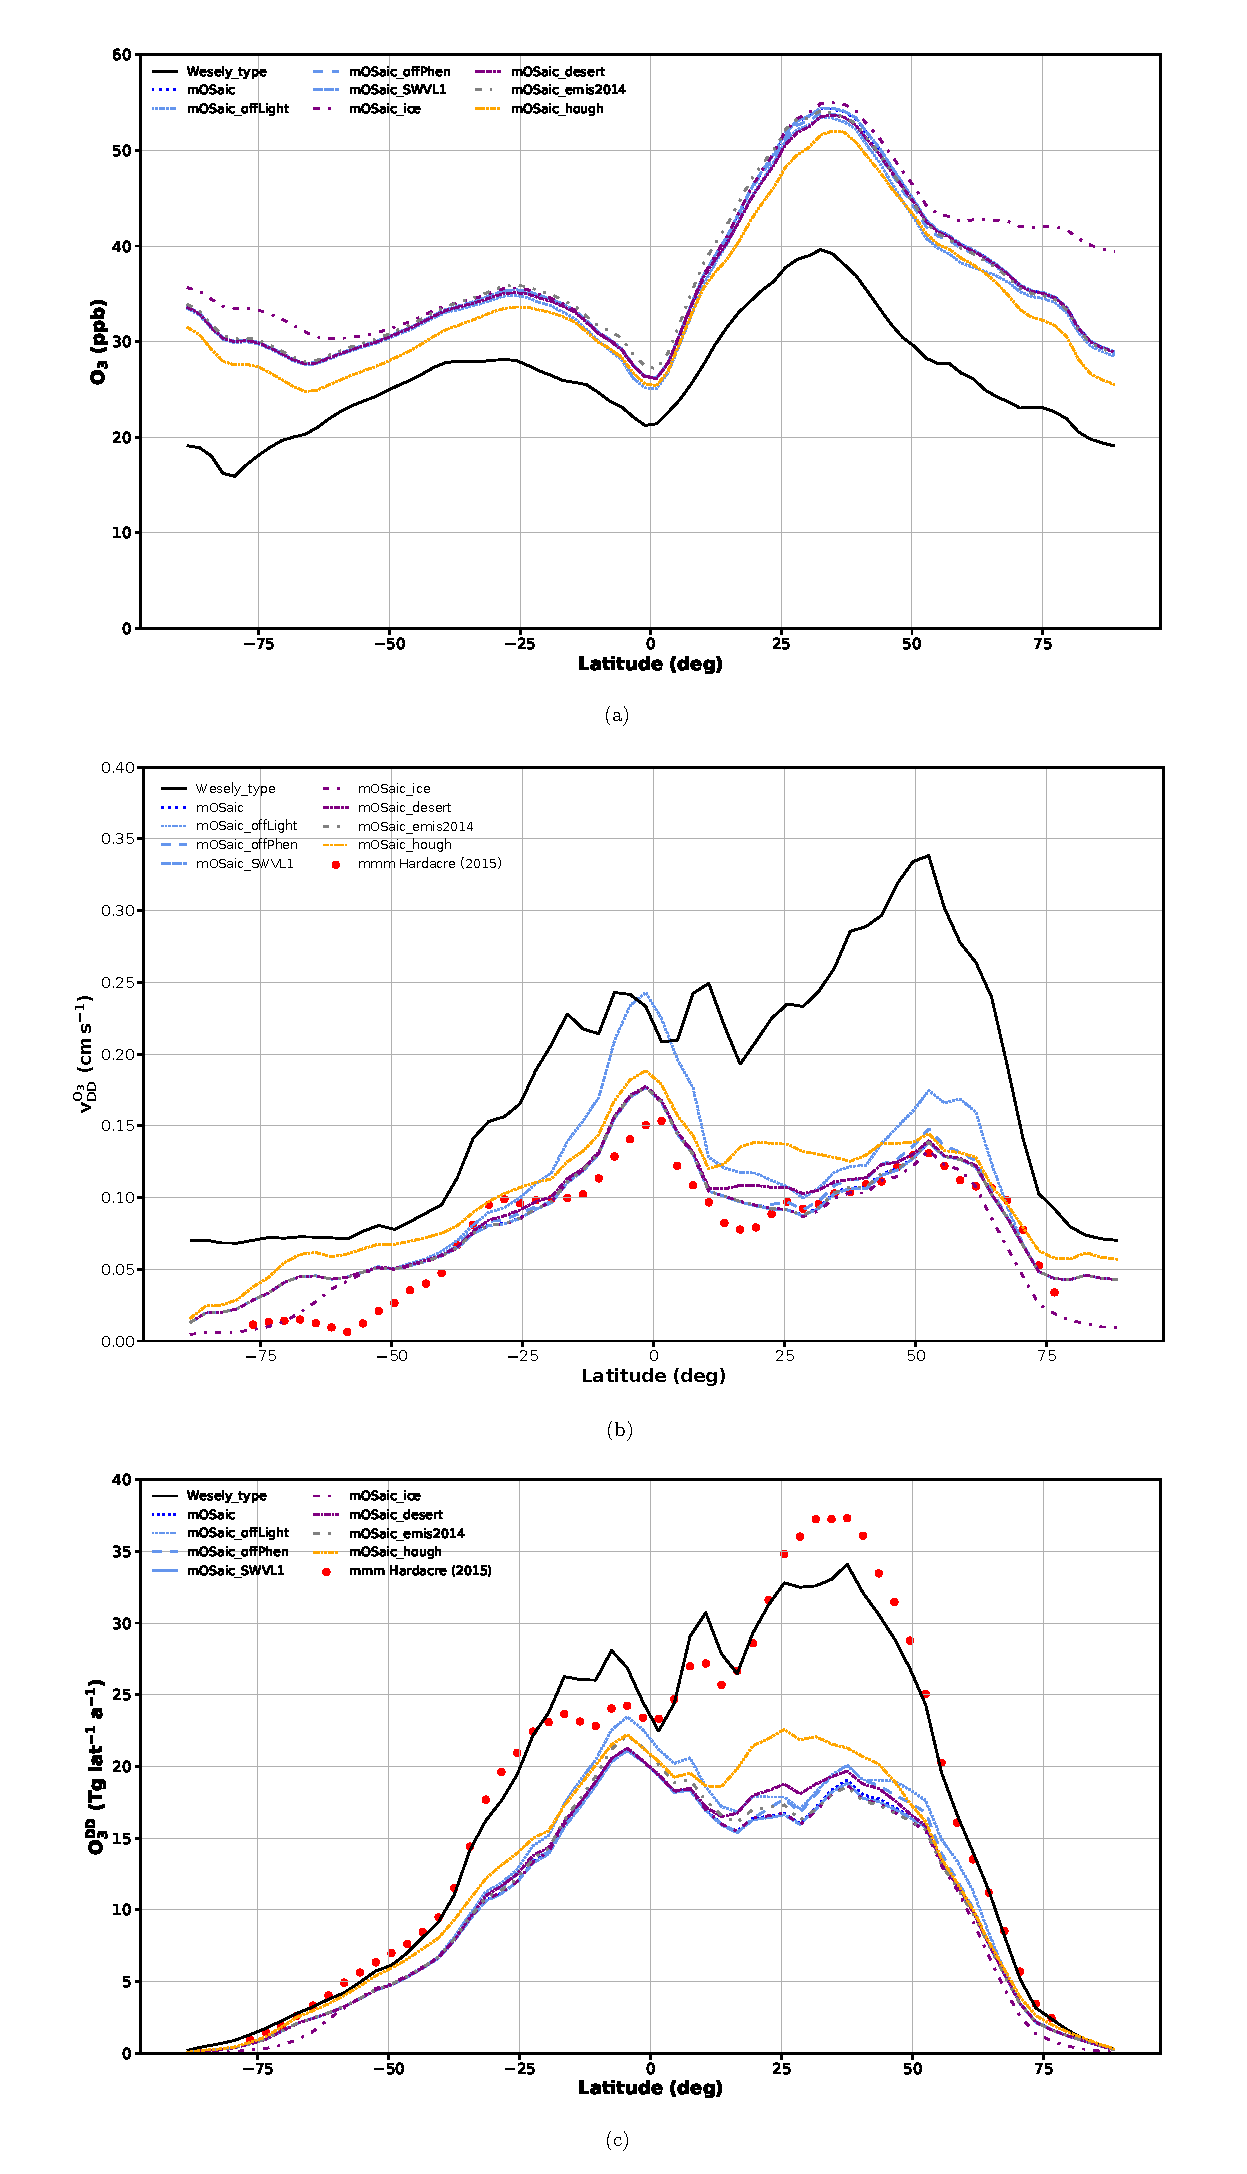
\includegraphics[width=8.3cm]{fig05}
  \caption{Comparison of the manifold of Oslo~CTM3 integrations with respect to (a) \DIFdelbeginFL \DIFdelFL{Surface ozone }\DIFdelendFL \DIFaddbeginFL \DIFaddFL{Ozone }\DIFaddendFL concentrations \DIFaddbeginFL \DIFaddFL{in the lowermost model level}\DIFaddendFL , (b) Annual average ozone dry deposition velocity, (c) Total annual ozone dry deposition. The different colors indicate sets of simulation with similar baselines. The multi-model mean from the evaluation of TF~HTAP models by \citet{ACP:Hardacre2015} is shown as a reference (where available).}
  \label{fig:mmm_drydep}
\end{figure}
%
In Appendix Fig.~\ref{fig:mmm_drydep_season}a, the average zonal ozone dry deposition is shown separated by month. Where available, we have added the multi-model-mean given by \citet{ACP:Hardacre2015} as reference. \DIFdelbegin \DIFdel{There }\DIFdelend \DIFaddbegin \DIFadd{As for the global annual comparisons above, the mOSaic scheme matches the multi-model-mean values remarkably well with respect to dry deposition velocities, while it strongly underestimates the total dry deposition. Qualitatively, there }\DIFaddend are two major phases apparent: NH and SH greening season. Spring and summer in the NH is reflected in a pronounced peak of $v_\text{DD}^\chem{O_3}$ in the northern mid latitudes, while it is absent in winter (SH summer). Spring and summer in the SH are marked by a southward shift of the tropical peak dry deposition velocity and a slight increase of $v_\text{DD}^\chem{O_3}$ in the region $(20-40)\,\unit{^\circ S}$. In the Wesely scheme, NH mid latitude peak velocities appear in June compared to July in the \DIFdelbegin \DIFdel{EMEP }\DIFdelend \DIFaddbegin \DIFadd{mOSaic }\DIFaddend scheme, indicating that the seasonal cycles differ. The corresponding total monthly ozone dry deposition is shown in Appendix Fig.~\ref{fig:mmm_drydep_season}b. In general, the seasonal patterns are quite similar in the Wesely scheme and the \DIFdelbegin \DIFdel{EMEP }\DIFdelend \DIFaddbegin \DIFadd{mOSaic }\DIFaddend scheme, displaying a strong symmetry around $10\,\unit{^\circ N}$ in January/February and November/December, respectively. What differs most is the molding and intensity of the NH peak dry deposition. Both schemes reach the maximum in June/July but the peak is much more differentiated in March already in the Wesely scheme. Similarly, the SH tropical peak dry deposition is reached in August/September but sustained longer, into October, in the Wesely scheme. Since we have not conducted any simulation with a meteorological year other than 2005, we cannot elaborate on whether this is a special feature of our chosen year or not.
\DIFdelbegin \DIFdel{In comparison, the available $2$ months of the multi-model-mean display a somewhat different pattern. Especially the NH/SH asymmetry is much more pronounced in February, than it is the EMEP scheme.
}\DIFdelend %
%%%%%%%%%%%%%%%%%%%%%%%%%%%%%%%%%%%%%%%%
\subsubsection{Average seasonal cycles}
\label{subsubsec:seasons}
%
To further disentangle the contributions of different regions to the global ozone budget, we will \DIFdelbegin \DIFdel{briefly }\DIFdelend look at different projections of seasonal cycles.

In Fig.~\ref{fig:mmm_drydep_hem}, the total annual ozone dry deposition separated into mid and high latitudes in the northern hemisphere ($30\,\unit{^\circ}-90\,\unit{^\circ N}$), the tropics and subtropics ($30\,\unit{^\circ S}-30\,\unit{^\circ N}$), and the mid and high latitudes in the southern hemisphere ($30\,\unit{^\circ}-90\,\unit{^\circ S}$) is shown. We have added the multi-model-mean by \citet{ACP:Hardacre2015} as reference. \DIFaddbegin \DIFadd{While the total ozone dry deposition of }\emph{\DIFadd{Wesely\_type}} \DIFadd{agrees well with the multi-model-mean in any zonal band, the mOSaic scheme displays a much smaller total ozone dry deposition. This deviation appears to be almost the same for each zonal band ($6-7\,\unit{\%}$).
}

\DIFaddend As expected, the NH mid and high latitudes display a strongly pronounced seasonal cycle, while it is less pronounced in the tropics (due to the lack of seasons) and in the SH (due to the small percentage of vegetated surface). The highest ozone dry deposition is found in the tropics and amounts on average to the  peak level of dry deposition in the NH for the multi-model-mean \citep{ACP:Hardacre2015} and \DIFdelbegin \DIFdel{EMEP }\DIFdelend \DIFaddbegin \DIFadd{mOSaic }\DIFaddend scheme. In the Wesely scheme, the average tropical ozone dry deposition diverges by \DIFdelbegin \DIFdel{about }\DIFdelend $5\,\unit{Tg}$ in comparison to its corresponding NH maximum. \DIFdelbegin \DIFdel{The }\DIFdelend \DIFaddbegin \DIFadd{Compared to the multi-model-mean, the }\DIFaddend seasonal cycle in the \DIFdelbegin \DIFdel{EMEP scheme }\DIFdelend \DIFaddbegin \DIFadd{Oslo~CTM3 NH }\DIFaddend appears to be shifted towards later in the year\DIFdelbegin \DIFdel{in the NH}\DIFdelend . The seasonal cycle in the tropics and subtropics \DIFdelbegin \DIFdel{is not changing, but the }\DIFdelend \DIFaddbegin \DIFadd{only differs by magnitude otherwise the shapes are identical for both the mOSaic scheme, the Wesely scheme, and the multi-model-mean. The }\DIFaddend total amount of dry deposition of ozone \DIFdelbegin \DIFdel{is very sensitive to differing realizations of the EMEP scheme, with }\DIFdelend \DIFaddbegin \DIFadd{differs strongly between the different model experiments, with }\DIFaddend \emph{\DIFdelbegin \DIFdel{EMEP}\DIFdelend \DIFaddbegin \DIFadd{mOSaic}\DIFaddend \_\DIFdelbegin \DIFdel{offLight}\DIFdelend \DIFaddbegin \DIFadd{SWVL1}\DIFaddend } and \emph{\DIFdelbegin \DIFdel{EMEP\_ppgs}\DIFdelend \DIFaddbegin \DIFadd{mOSaic}\DIFaddend \_\DIFdelbegin \DIFdel{2005}\DIFdelend \DIFaddbegin \DIFadd{hough}\DIFaddend } displaying the \DIFdelbegin \DIFdel{highest and the lowest }\DIFdelend \DIFaddbegin \DIFadd{lowest and highest }\DIFaddend amount, respectively. This indicates that surface ozone \DIFaddbegin \DIFadd{is much more sensitive to the choice of parameters ($\mathcal{O}(5\,\unit{ppb})$ for }\emph{\DIFadd{mOSaic\_hough}} \DIFaddend in the tropics\DIFdelbegin \DIFdel{may be very sensitive to changes in emissions of ozone precursors and changes in long-wave radiative transfer (e.g., due changes in cloud cover or aerosol}\DIFdelend \DIFaddbegin \DIFadd{) than to slight changes in precursor emissions ($\mathcal{O}(1\,\unit{ppb})$ for }\emph{\DIFadd{mOSaic\_emis2014}} \DIFadd{in the tropics}\DIFaddend ).

As suggested by \citet{ACP:Hardacre2015}, we \DIFdelbegin \DIFdel{retrospectively separate }\DIFdelend \DIFaddbegin \DIFadd{also look at }\DIFaddend ozone dry deposition velocities with respect to surface types \DIFaddbegin \DIFadd{separately. Since dry deposition velocities are not directly available for }\emph{\DIFadd{Wesely\_type}}\DIFadd{, we use Eq.~(\ref{eq:retro_vdd}) to estimate these}\DIFaddend . Based on a CLM~2 average dynamic land surface map, we \DIFdelbegin \DIFdel{generated }\DIFdelend \DIFaddbegin \DIFadd{generate }\DIFaddend masks for 9 different surface types (Fig.~\ref{fig:pft_landsurface}a\DIFdelbegin \DIFdel{and used }\DIFdelend \DIFaddbegin \DIFadd{) and use }\DIFaddend these to select gridboxes with a high percentage of these surface types, ranging from a meager $70\,\unit{\%}$ for cropland in the NH mid latitudes to $100\,\unit{\%}$ regarding desert, ocean, snow and ice, and tropical forest. Thus, it \DIFdelbegin \DIFdel{was }\DIFdelend \DIFaddbegin \DIFadd{is }\DIFaddend not possible to exclusively select gridboxes with $100\,\unit{\%}$ cover for each surface type. Since we have not performed a full unfolding on the data, the results should be treated with slight caution \DIFaddbegin \DIFadd{(e.g. over cropland). In case of the mOSaic scheme, we have pre-selected the dry deposition velocities in accordance to the land surface type}\DIFaddend .
%
\begin{figure*}[t]
  \includegraphics[width=12cm]{fig06}
  \caption{Seasonal cycle of total annual amount of ozone removed from the atmosphere through dry deposition separated into northern hemisphere (NH), tropics (TR), and southern hemisphere (SH). The multi-model mean from the evaluation of HTAP models by \citet{ACP:Hardacre2015} is shown as a reference.}
  \label{fig:mmm_drydep_hem}
\end{figure*}
%
\DIFaddbegin 

\DIFaddend In Fig.~\ref{fig:mmm_drydep_season_pft}, the seasonal cycles of dry deposition velocities are shown for the nine surface categories. The patterns and absolute numbers differ substantially between the Wesely scheme and the \DIFdelbegin \DIFdel{EMEP }\DIFdelend \DIFaddbegin \DIFadd{mOSaic }\DIFaddend scheme and the multi-model-mean. The divergence of the average dry deposition velocities between \DIFdelbegin \DIFdel{the Wesely scheme and the EMEP scheme }\DIFdelend \DIFaddbegin \emph{\DIFadd{Wesely\_type}} \DIFadd{and }\emph{\DIFadd{mOSaic}} \DIFaddend in desert regions (\DIFdelbegin \DIFdel{$\Delta \overline{v}_\text{desert}^\chem{O_3} = 0.18\,\unit{cm\,s^{-1}}$}\DIFdelend \DIFaddbegin \DIFadd{$\Delta \overline{v}_\text{desert}^\chem{O_3} = 0.20\,\unit{cm\,s^{-1}}$}\DIFaddend ) as well as grassland (\DIFdelbegin \DIFdel{$\Delta \overline{v}_\text{grassland}^\chem{O_3} = 0.54\,\unit{cm\,s^{-1}}$}\DIFdelend \DIFaddbegin \DIFadd{$\Delta \overline{v}_\text{grassland}^\chem{O_3} = 0.65\,\unit{cm\,s^{-1}}$}\DIFaddend ) is quite remarkable\DIFdelbegin \DIFdel{as well as the difference of both }\DIFdelend \DIFaddbegin \DIFadd{. The difference of }\emph{\DIFadd{mOSaic}} \DIFadd{and }\emph{\DIFadd{Wesely\_type}} \DIFaddend to the multi-model-mean in tropical forest regions \DIFdelbegin \DIFdel{($\Delta \overline{v}_\text{tropical forest}^\chem{O_3} = 0.49\,\unit{cm\,s^{-1}}$). In contrast to the Wesely scheme and the EMEP scheme, the }\DIFdelend \DIFaddbegin \DIFadd{is $\Delta_\text{mOSaic} \overline{v}_\text{tropical forest}^\chem{O_3} = 0.61\,\unit{cm\,s^{-1}}$ and $\Delta_\text{Wesely\_type} \overline{v}_\text{tropical forest}^\chem{O_3} = 0.49\,\unit{cm\,s^{-1}}$, respectively. The }\DIFaddend multi-model-mean \DIFdelbegin \DIFdel{indicates }\DIFdelend \DIFaddbegin \DIFadd{displays }\DIFaddend a rather pronounced seasonal cycle in desert regions ($0.10\,\unit{cm\,s^{-1}} \leq v^\chem{O_3}_\text{desert}\leq 0.15\,\unit{cm\,s^{-1}}$)\DIFdelbegin \DIFdel{. The estimated }\DIFdelend \DIFaddbegin \DIFadd{, which cannot be reproduced with the mOSaic scheme. The }\DIFaddend dry deposition velocities over desert regions are consistent with the \DIFdelbegin \DIFdel{previously mentioned baseline values of ozone dry deposition}\DIFdelend \DIFaddbegin \DIFadd{average values from the prescribed ozone surface resistances}\DIFaddend , which means that in the \DIFdelbegin \DIFdel{EMEP }\DIFdelend \DIFaddbegin \DIFadd{mOSaic }\DIFaddend scheme they are \DIFdelbegin \DIFdel{about }\DIFdelend $1$ order of magnitude lower than in the Wesely scheme. \DIFaddbegin \DIFadd{In the mOSaic scheme, dry deposition to deserts is dominated by contribution from $R_b$. }\DIFaddend From a limited number of ozone flux measurements in the Sahara desert, \citet{AE:Gusten1995} deduced $v^\chem{O_3}_\text{desert, day} = 0.1\,\unit{cm\,s^{-1}}$, $v^\chem{O_3}_\text{desert, night} = 0.04\,\unit{cm\,s^{-1}}$, and $\overline{v}^\chem{O_3}_\text{desert} = 0.065\,\unit{cm\,s^{-1}}$. This implies, that ozone dry deposition over desert regions is highly overestimated in the Wesely scheme as well as in TF~HTAP models, while it may be underestimated in the \DIFdelbegin \DIFdel{EMEP }\DIFdelend \DIFaddbegin \DIFadd{mOSaic }\DIFaddend scheme. Similarly, the dry deposition velocities over water differ. From measurements during ship-campaigns a mean value of $\overline{v}^\chem{O_3}_\text{water} = 0.019\,\unit{cm\,s^{-1}}$ over the ocean has been deduced \citep{JGR:Helmig2012}. In a model study of different mechanisms of dry deposition to ocean waters by means of prescribed $\overline{v}_\text{water}^\chem{O_3}$ and one- and two-layer gas exchange modeling, \citet{ACP:Luhar2017} found $\overline{v}_\text{water}^\chem{O_3}$ ranging between $0.018\,\unit{cm\,s^{-1}}$ (two-layer scheme) and $0.039\,\unit{cm\,s^{-1}}$ (prescribed). With $\overline{v}^\chem{O_3}_\text{water} = (0.046\pm0.002)\,\unit{cm\,s^{-1}}$, the \DIFdelbegin \DIFdel{EMEP }\DIFdelend \DIFaddbegin \DIFadd{mOSaic }\DIFaddend scheme (Section~\ref{subsubsec:Rb}) yields probably a too strong dry deposition to ocean\DIFdelbegin \DIFdel{which }\DIFdelend \DIFaddbegin \DIFadd{, but is in line with the multi-model-mean. This }\DIFaddend implies that ozone concentrations might even become larger and dry deposition even lower in the model if a \DIFdelbegin \DIFdel{two-layer scheme }\DIFdelend \DIFaddbegin \DIFadd{more advanced dry deposition scheme to the ocean }\DIFaddend would be implemented. With respect to vegetation, we might be able to improve the model performance further by allowing more PFTs and phenologies, especially in regions covered by tropical \DIFdelbegin \DIFdel{or coniferous forest \mbox{%DIFAUXCMD
\citep{GCB:Anav2017} }\hspace{0pt}%DIFAUXCMD
}\DIFdelend \DIFaddbegin \DIFadd{forest \mbox{%DIFAUXCMD
\citep{GCB:Anav2017} }\hspace{0pt}%DIFAUXCMD
or in boreal regions}\DIFaddend . 
%
\begin{figure*}[t]
  \includegraphics[width=12cm]{fig07}
  \caption{Average seasonal cycles of ozone dry deposition velocities separated by land use type. Results from \citep{ACP:Hardacre2015} are shown as a reference. We refrain from showing the full extent of \emph{EMEP\_offLight} here, since it is an extreme scenario and has been discussed already.}
  \label{fig:mmm_drydep_season_pft}
\end{figure*}
%

Finally, we take a look at the different global as well as hemispheric dry deposition sinks for ozone (Table~\ref{tab:ozone_sinks}). Despite its vastness, the ocean amounts only to \DIFdelbegin \DIFdel{about $23\,\unit{\%}$ }\DIFdelend \DIFaddbegin \DIFadd{$35\,\unit{\%}$ }\DIFaddend of the global ozone sink due to dry deposition in the Oslo~CTM3 with operative \DIFdelbegin \DIFdel{EMEP scheme , while }\DIFdelend \DIFaddbegin \DIFadd{mOSaic scheme (}\emph{\DIFadd{mOSaic}}\DIFadd{), while permanently }\DIFaddend ice and snow \DIFdelbegin \DIFdel{account for far less than $1\,\unit{\%}$}\DIFdelend \DIFaddbegin \DIFadd{covered regions account for $1.2\,\unit{\%}$}\DIFaddend . The remainder is deposited to \DIFdelbegin \DIFdel{various other }\DIFdelend land surfaces of which deserts might be the most neglected in process-modeling. The total annual dry deposition in the \DIFdelbegin \DIFdel{EMEP scheme is about }\DIFdelend \DIFaddbegin \DIFadd{mOSaic scheme is }\DIFaddend one-third below the multi-model-mean result by \citet{ACP:Hardacre2015}. But also the results of \DIFdelbegin \DIFdel{\mbox{%DIFAUXCMD
\citet{ACP:Luhar2017} }\hspace{0pt}%DIFAUXCMD
}\DIFdelend \DIFaddbegin \DIFadd{\mbox{%DIFAUXCMD
\citet{ACP:Luhar2017, ACP:Luhar2018} }\hspace{0pt}%DIFAUXCMD
}\DIFaddend yield a $(19-27)\,\unit{\%}$ lower ozone dry deposition than the models participating in the model intercomparison, with deposition to ocean ranging between $(12-21)\,\unit{\%}$ \DIFaddbegin \DIFadd{of the total annual ozone dry deposition. In particular, \mbox{%DIFAUXCMD
\citet{ACP:Luhar2018} }\hspace{0pt}%DIFAUXCMD
found that current model estimates of ozone dry deposition to the ocean may be three times too high compared to their analysis. This implies that the ozone dry deposition to the ocean the Oslo~CTM3 is too high as well}\DIFaddend .
%
\begin{table*}[t]
  \caption{Total ozone dry deposition for the respective \DIFdelbeginFL \DIFdelFL{year }\DIFdelendFL \DIFaddbeginFL \DIFaddFL{model experiment }\DIFaddendFL in \unit{Tg\,a^{-1}}\DIFdelbeginFL \DIFdelFL{separated into }\DIFdelendFL \DIFaddbeginFL \DIFaddFL{. The global ozone dry deposition has been weighted by }\DIFaddendFL ocean, ice and, land \DIFdelbeginFL \DIFdelFL{contributions}\DIFdelendFL \DIFaddbeginFL \DIFaddFL{fraction in each gridbox, respectively. }\emph{\DIFaddFL{Ice}} \DIFaddFL{herein refers to regions at high latitudes that are permanently covered by ice and snow}\DIFaddendFL .}
  \DIFdelbeginFL %DIFDELCMD < \begin{tabular}{lccccccccccccr}
%DIFDELCMD < %%%
\DIFdelendFL \DIFaddbeginFL \begin{tabular}{lccccccccc|cccr}
    \DIFaddendFL \tophline
    \DIFdelbeginFL %DIFDELCMD < \multirow{3}{*}{Simulation} %%%
\DIFdelendFL \DIFaddbeginFL \multirow{3}{*}{Experiment} \DIFaddendFL & \multicolumn{3}{c}{Ocean} & \multicolumn{3}{c}{Ice} & \multicolumn{3}{c}{Land} & \multicolumn{3}{c}{Total} & $\Delta^\dagger$\\
    & NH & SH & Global & NH & SH & Global & NH & SH & Global & NH & SH & Global\\
    & \multicolumn{3}{c}{(\unit{Tg\,a^{-1}})} & \multicolumn{3}{c}{(\unit{Tg\,a^{-1}})} & \multicolumn{3}{c}{(\unit{Tg\,a^{-1}})} & \multicolumn{3}{c}{(\unit{Tg\,a^{-1}})} & (\unit{\%})\\
    \middlehline
    Wesely\_type & \DIFdelbeginFL \DIFdelFL{88.7 }\DIFdelendFL \DIFaddbeginFL \DIFaddFL{160.5 }\DIFaddendFL & \DIFdelbeginFL \DIFdelFL{110.3 }\DIFdelendFL \DIFaddbeginFL \DIFaddFL{147.7 }\DIFaddendFL & \DIFdelbeginFL \DIFdelFL{199.0 }\DIFdelendFL \DIFaddbeginFL \DIFaddFL{308.2 }\DIFaddendFL & \DIFdelbeginFL \DIFdelFL{0.7 }\DIFdelendFL \DIFaddbeginFL \DIFaddFL{7.0 }\DIFaddendFL & \DIFdelbeginFL \DIFdelFL{5.0 }\DIFdelendFL \DIFaddbeginFL \DIFaddFL{6.4 }\DIFaddendFL & \DIFdelbeginFL \DIFdelFL{5.7 }\DIFdelendFL \DIFaddbeginFL \DIFaddFL{13.4 }\DIFaddendFL & \DIFdelbeginFL \DIFdelFL{346.1 }\DIFdelendFL \DIFaddbeginFL \DIFaddFL{417.3 }\DIFaddendFL & \DIFdelbeginFL \DIFdelFL{153.5 }\DIFdelendFL \DIFaddbeginFL \DIFaddFL{190.8 }\DIFaddendFL & \DIFdelbeginFL \DIFdelFL{499.6 }\DIFdelendFL \DIFaddbeginFL \DIFaddFL{608.2 }\DIFaddendFL & \DIFdelbeginFL \DIFdelFL{612.4 }\DIFdelendFL \DIFaddbeginFL \DIFaddFL{613.4 }\DIFaddendFL & \DIFdelbeginFL \DIFdelFL{347.9 }\DIFdelendFL \DIFaddbeginFL \DIFaddFL{344.9 }\DIFaddendFL & \DIFdelbeginFL \DIFdelFL{960.2 }\DIFdelendFL \DIFaddbeginFL \DIFaddFL{958.3 }\DIFaddendFL & \DIFdelbeginFL \DIFdelFL{46.8}\DIFdelendFL \DIFaddbeginFL \DIFaddFL{36.7}\DIFaddendFL \\
    \DIFdelbeginFL \DIFdelFL{EMEP\_full }\DIFdelendFL \DIFaddbeginFL \DIFaddFL{mOSaic }\DIFaddendFL & \DIFdelbeginFL \DIFdelFL{67.1 }\DIFdelendFL \DIFaddbeginFL \DIFaddFL{108.1 }\DIFaddendFL & \DIFdelbeginFL \DIFdelFL{84.7 }\DIFdelendFL \DIFaddbeginFL \DIFaddFL{105.3 }\DIFaddendFL & \DIFdelbeginFL \DIFdelFL{151.8 }\DIFdelendFL \DIFaddbeginFL \DIFaddFL{213.4 }\DIFaddendFL & \DIFdelbeginFL \DIFdelFL{0.6 }\DIFdelendFL \DIFaddbeginFL \DIFaddFL{4.3 }\DIFaddendFL & \DIFdelbeginFL \DIFdelFL{4.4 }\DIFdelendFL \DIFaddbeginFL \DIFaddFL{3.1 }\DIFaddendFL & \DIFdelbeginFL \DIFdelFL{5.0 }\DIFdelendFL \DIFaddbeginFL \DIFaddFL{7.4 }\DIFaddendFL & \DIFdelbeginFL \DIFdelFL{236.0 }\DIFdelendFL \DIFaddbeginFL \DIFaddFL{236.2 }\DIFaddendFL & \DIFdelbeginFL \DIFdelFL{112.3 }\DIFdelendFL \DIFaddbeginFL \DIFaddFL{130.3 }\DIFaddendFL & \DIFdelbeginFL \DIFdelFL{348.2 }\DIFdelendFL \DIFaddbeginFL \DIFaddFL{366.4 }\DIFaddendFL & \DIFdelbeginFL \DIFdelFL{408.6 }\DIFdelendFL \DIFaddbeginFL \DIFaddFL{368.3 }\DIFaddendFL & \DIFdelbeginFL \DIFdelFL{245.6 }\DIFdelendFL \DIFaddbeginFL \DIFaddFL{238.6 }\DIFaddendFL & \DIFdelbeginFL \DIFdelFL{654.2 }\DIFdelendFL \DIFaddbeginFL \DIFaddFL{606.9 }\DIFaddendFL & 0.0\\
    \DIFdelbeginFL \DIFdelFL{EMEP}\DIFdelendFL \DIFaddbeginFL \DIFaddFL{mOSaic}\DIFaddendFL \_offLight & \DIFdelbeginFL \DIFdelFL{66.6 }\DIFdelendFL \DIFaddbeginFL \DIFaddFL{110.5 }\DIFaddendFL & \DIFdelbeginFL \DIFdelFL{84.1 }\DIFdelendFL \DIFaddbeginFL \DIFaddFL{106.3 }\DIFaddendFL & \DIFdelbeginFL \DIFdelFL{150.7 }\DIFdelendFL \DIFaddbeginFL \DIFaddFL{216.8 }\DIFaddendFL & \DIFdelbeginFL \DIFdelFL{0.6 }\DIFdelendFL \DIFaddbeginFL \DIFaddFL{4.3 }\DIFaddendFL & \DIFdelbeginFL \DIFdelFL{4.4 }\DIFdelendFL \DIFaddbeginFL \DIFaddFL{3.0 }\DIFaddendFL & \DIFdelbeginFL \DIFdelFL{5.0 }\DIFdelendFL \DIFaddbeginFL \DIFaddFL{7.4 }\DIFaddendFL & \DIFdelbeginFL \DIFdelFL{267.8 }\DIFdelendFL \DIFaddbeginFL \DIFaddFL{263.1 }\DIFaddendFL & \DIFdelbeginFL \DIFdelFL{129.8 }\DIFdelendFL \DIFaddbeginFL \DIFaddFL{145.3 }\DIFaddendFL & \DIFdelbeginFL \DIFdelFL{397.6 }\DIFdelendFL \DIFaddbeginFL \DIFaddFL{408.4 }\DIFaddendFL & \DIFdelbeginFL \DIFdelFL{451.3 }\DIFdelendFL \DIFaddbeginFL \DIFaddFL{399.9 }\DIFaddendFL & \DIFdelbeginFL \DIFdelFL{267.2 }\DIFdelendFL \DIFaddbeginFL \DIFaddFL{254.7 }\DIFaddendFL & \DIFdelbeginFL \DIFdelFL{718.6 }\DIFdelendFL \DIFaddbeginFL \DIFaddFL{654.6 }\DIFaddendFL & \DIFdelbeginFL \DIFdelFL{9.8}\DIFdelendFL \DIFaddbeginFL \DIFaddFL{7.3}\DIFaddendFL \\
    \DIFdelbeginFL \DIFdelFL{EMEP}\DIFdelendFL \DIFaddbeginFL \DIFaddFL{mOSaic}\DIFaddendFL \_offPhen & \DIFdelbeginFL \DIFdelFL{67.1 }\DIFdelendFL \DIFaddbeginFL \DIFaddFL{108.3 }\DIFaddendFL & \DIFdelbeginFL \DIFdelFL{84.6 }\DIFdelendFL \DIFaddbeginFL \DIFaddFL{105.3 }\DIFaddendFL & \DIFdelbeginFL \DIFdelFL{151.7 }\DIFdelendFL \DIFaddbeginFL \DIFaddFL{213.6 }\DIFaddendFL & \DIFdelbeginFL \DIFdelFL{0.6 }\DIFdelendFL \DIFaddbeginFL \DIFaddFL{4.3 }\DIFaddendFL & \DIFdelbeginFL \DIFdelFL{4.4 }\DIFdelendFL \DIFaddbeginFL \DIFaddFL{3.1 }\DIFaddendFL & \DIFdelbeginFL \DIFdelFL{5.0 }\DIFdelendFL \DIFaddbeginFL \DIFaddFL{7.4 }\DIFaddendFL & \DIFdelbeginFL \DIFdelFL{239.9 }\DIFdelendFL \DIFaddbeginFL \DIFaddFL{246.9 }\DIFaddendFL & \DIFdelbeginFL \DIFdelFL{116.0 }\DIFdelendFL \DIFaddbeginFL \DIFaddFL{132.2 }\DIFaddendFL & \DIFdelbeginFL \DIFdelFL{355.9 }\DIFdelendFL \DIFaddbeginFL \DIFaddFL{379.1 }\DIFaddendFL & \DIFdelbeginFL \DIFdelFL{413.9 }\DIFdelendFL \DIFaddbeginFL \DIFaddFL{379.5 }\DIFaddendFL & \DIFdelbeginFL \DIFdelFL{249.9 }\DIFdelendFL \DIFaddbeginFL \DIFaddFL{240.5 }\DIFaddendFL & \DIFdelbeginFL \DIFdelFL{663.7 }\DIFdelendFL \DIFaddbeginFL \DIFaddFL{620.0 }\DIFaddendFL & \DIFdelbeginFL \DIFdelFL{1.5}\DIFdelendFL \DIFaddbeginFL \DIFaddFL{2.1}\DIFaddendFL \\
    \DIFdelbeginFL \DIFdelFL{EMEP\_SWVL4 }\DIFdelendFL \DIFaddbeginFL \DIFaddFL{mOSaic\_SWVL1 }\DIFaddendFL & \DIFdelbeginFL \DIFdelFL{68.1 }\DIFdelendFL \DIFaddbeginFL \DIFaddFL{108.1 }\DIFaddendFL & \DIFdelbeginFL \DIFdelFL{86.1 }\DIFdelendFL \DIFaddbeginFL \DIFaddFL{105.2 }\DIFaddendFL & \DIFdelbeginFL \DIFdelFL{154.2 }\DIFdelendFL \DIFaddbeginFL \DIFaddFL{213.3 }\DIFaddendFL & \DIFdelbeginFL \DIFdelFL{0.6 }\DIFdelendFL \DIFaddbeginFL \DIFaddFL{4.3 }\DIFaddendFL & \DIFdelbeginFL \DIFdelFL{4.5 }\DIFdelendFL \DIFaddbeginFL \DIFaddFL{3.1 }\DIFaddendFL & \DIFdelbeginFL \DIFdelFL{5.1 }\DIFdelendFL \DIFaddbeginFL \DIFaddFL{7.4 }\DIFaddendFL & \DIFdelbeginFL \DIFdelFL{241.8 }\DIFdelendFL \DIFaddbeginFL \DIFaddFL{234.6 }\DIFaddendFL & \DIFdelbeginFL \DIFdelFL{115.0 }\DIFdelendFL \DIFaddbeginFL \DIFaddFL{128.8 }\DIFaddendFL & \DIFdelbeginFL \DIFdelFL{356.8 }\DIFdelendFL \DIFaddbeginFL \DIFaddFL{363.4 }\DIFaddendFL & \DIFdelbeginFL \DIFdelFL{417.2 }\DIFdelendFL \DIFaddbeginFL \DIFaddFL{366.6 }\DIFaddendFL & \DIFdelbeginFL \DIFdelFL{250.7 }\DIFdelendFL \DIFaddbeginFL \DIFaddFL{237.1 }\DIFaddendFL & \DIFdelbeginFL \DIFdelFL{667.9 }\DIFdelendFL \DIFaddbeginFL \DIFaddFL{603.7 }\DIFaddendFL & \DIFdelbeginFL \DIFdelFL{2.1}\DIFdelendFL \DIFaddbeginFL \DIFaddFL{-0.5}\DIFaddendFL \\
    \DIFdelbeginFL \DIFdelFL{EMEP\_ppgs }\DIFdelendFL \DIFaddbeginFL \DIFaddFL{mOSaic\_ice }\DIFaddendFL & \DIFdelbeginFL \DIFdelFL{67.1 }\DIFdelendFL \DIFaddbeginFL \DIFaddFL{105.6 }\DIFaddendFL & \DIFdelbeginFL \DIFdelFL{84.6 }\DIFdelendFL \DIFaddbeginFL \DIFaddFL{103.0 }\DIFaddendFL & \DIFdelbeginFL \DIFdelFL{151.7 }\DIFdelendFL \DIFaddbeginFL \DIFaddFL{208.6 }\DIFaddendFL & \DIFdelbeginFL \DIFdelFL{0.6 }\DIFdelendFL \DIFaddbeginFL \DIFaddFL{2.6 }\DIFaddendFL & \DIFdelbeginFL \DIFdelFL{4.4 }\DIFdelendFL \DIFaddbeginFL \DIFaddFL{1.0 }\DIFaddendFL & \DIFdelbeginFL \DIFdelFL{5.0 }\DIFdelendFL \DIFaddbeginFL \DIFaddFL{3.6 }\DIFaddendFL & \DIFdelbeginFL \DIFdelFL{238.7 }\DIFdelendFL \DIFaddbeginFL \DIFaddFL{232.7 }\DIFaddendFL & \DIFdelbeginFL \DIFdelFL{112.6 }\DIFdelendFL \DIFaddbeginFL \DIFaddFL{130.2 }\DIFaddendFL & \DIFdelbeginFL \DIFdelFL{351.3 }\DIFdelendFL \DIFaddbeginFL \DIFaddFL{362.9 }\DIFaddendFL & \DIFdelbeginFL \DIFdelFL{411.4 }\DIFdelendFL \DIFaddbeginFL \DIFaddFL{358.3 }\DIFaddendFL & \DIFdelbeginFL \DIFdelFL{246.0 }\DIFdelendFL \DIFaddbeginFL \DIFaddFL{234.2 }\DIFaddendFL & \DIFdelbeginFL \DIFdelFL{657.4 }\DIFdelendFL \DIFaddbeginFL \DIFaddFL{592.6 }\DIFaddendFL & \DIFdelbeginFL \DIFdelFL{0.5}\DIFdelendFL \DIFaddbeginFL \DIFaddFL{-2.4}\DIFaddendFL \\
    \DIFdelbeginFL \DIFdelFL{EMEP\_ppgssh }\DIFdelendFL \DIFaddbeginFL \DIFaddFL{mOSaic\_desert }\DIFaddendFL & \DIFdelbeginFL \DIFdelFL{67.0 }\DIFdelendFL \DIFaddbeginFL \DIFaddFL{109.1 }\DIFaddendFL & \DIFdelbeginFL \DIFdelFL{84.5 }\DIFdelendFL \DIFaddbeginFL \DIFaddFL{105.5 }\DIFaddendFL & \DIFdelbeginFL \DIFdelFL{151.6 }\DIFdelendFL \DIFaddbeginFL \DIFaddFL{214.6 }\DIFaddendFL & \DIFdelbeginFL \DIFdelFL{0.6 }\DIFdelendFL \DIFaddbeginFL \DIFaddFL{4.3 }\DIFaddendFL & \DIFdelbeginFL \DIFdelFL{4.4 }\DIFdelendFL \DIFaddbeginFL \DIFaddFL{3.1 }\DIFaddendFL & \DIFdelbeginFL \DIFdelFL{5.0 }\DIFdelendFL \DIFaddbeginFL \DIFaddFL{7.4 }\DIFaddendFL & \DIFdelbeginFL \DIFdelFL{243.9 }\DIFdelendFL \DIFaddbeginFL \DIFaddFL{250.4 }\DIFaddendFL & \DIFdelbeginFL \DIFdelFL{119.4 }\DIFdelendFL \DIFaddbeginFL \DIFaddFL{132.6 }\DIFaddendFL & \DIFdelbeginFL \DIFdelFL{363.3 }\DIFdelendFL \DIFaddbeginFL \DIFaddFL{383.0 }\DIFaddendFL & \DIFdelbeginFL \DIFdelFL{419.4 }\DIFdelendFL \DIFaddbeginFL \DIFaddFL{383.4 }\DIFaddendFL & \DIFdelbeginFL \DIFdelFL{253.6 }\DIFdelendFL \DIFaddbeginFL \DIFaddFL{241.2 }\DIFaddendFL & \DIFdelbeginFL \DIFdelFL{673.0 }\DIFdelendFL \DIFaddbeginFL \DIFaddFL{624.6 }\DIFaddendFL & \DIFdelbeginFL \DIFdelFL{2.9}\DIFdelendFL \DIFaddbeginFL \DIFaddFL{2.8}\DIFaddendFL \\
    \DIFdelbeginFL \DIFdelFL{EMEP\_ppgssh\_ice }\DIFdelendFL \DIFaddbeginFL \DIFaddFL{mOSaic\_emis2014 }\DIFaddendFL & \DIFdelbeginFL \DIFdelFL{66.5 }\DIFdelendFL \DIFaddbeginFL \DIFaddFL{108.9 }\DIFaddendFL & \DIFdelbeginFL \DIFdelFL{84.8 }\DIFdelendFL \DIFaddbeginFL \DIFaddFL{107.0 }\DIFaddendFL & \DIFdelbeginFL \DIFdelFL{151.3 }\DIFdelendFL \DIFaddbeginFL \DIFaddFL{215.9 }\DIFaddendFL & \DIFdelbeginFL \DIFdelFL{0.2 }\DIFdelendFL \DIFaddbeginFL \DIFaddFL{4.3 }\DIFaddendFL & \DIFdelbeginFL \DIFdelFL{1.3 }\DIFdelendFL \DIFaddbeginFL \DIFaddFL{3.1 }\DIFaddendFL & \DIFdelbeginFL \DIFdelFL{1.4 }\DIFdelendFL \DIFaddbeginFL \DIFaddFL{7.3 }\DIFaddendFL & \DIFdelbeginFL \DIFdelFL{240.3 }\DIFdelendFL \DIFaddbeginFL \DIFaddFL{238.3 }\DIFaddendFL & \DIFdelbeginFL \DIFdelFL{120.4 }\DIFdelendFL \DIFaddbeginFL \DIFaddFL{133.8 }\DIFaddendFL & \DIFdelbeginFL \DIFdelFL{360.7 }\DIFdelendFL \DIFaddbeginFL \DIFaddFL{372.1 }\DIFaddendFL & \DIFdelbeginFL \DIFdelFL{413.0 }\DIFdelendFL \DIFaddbeginFL \DIFaddFL{370.8 }\DIFaddendFL & \DIFdelbeginFL \DIFdelFL{251.1 }\DIFdelendFL \DIFaddbeginFL \DIFaddFL{243.9 }\DIFaddendFL & \DIFdelbeginFL \DIFdelFL{664.1 }\DIFdelendFL \DIFaddbeginFL \DIFaddFL{614.7 }\DIFaddendFL & \DIFdelbeginFL \DIFdelFL{1.5}\DIFdelendFL \DIFaddbeginFL \DIFaddFL{1.3}\DIFaddendFL \\
    \DIFdelbeginFL \DIFdelFL{EMEP\_ppgs\_2005 }\DIFdelendFL \DIFaddbeginFL \DIFaddFL{mOSaic\_hough }\DIFaddendFL & \DIFdelbeginFL \DIFdelFL{66.8 }\DIFdelendFL \DIFaddbeginFL \DIFaddFL{133.3 }\DIFaddendFL & \DIFdelbeginFL \DIFdelFL{83.5 }\DIFdelendFL \DIFaddbeginFL \DIFaddFL{131.1 }\DIFaddendFL & \DIFdelbeginFL \DIFdelFL{150.4 }\DIFdelendFL \DIFaddbeginFL \DIFaddFL{264.4 }\DIFaddendFL & \DIFdelbeginFL \DIFdelFL{0.6 }\DIFdelendFL \DIFaddbeginFL \DIFaddFL{4.9 }\DIFaddendFL & \DIFdelbeginFL \DIFdelFL{4.4 }\DIFdelendFL \DIFaddbeginFL \DIFaddFL{3.6 }\DIFaddendFL & \DIFdelbeginFL \DIFdelFL{5.0 }\DIFdelendFL \DIFaddbeginFL \DIFaddFL{8.4 }\DIFaddendFL & \DIFdelbeginFL \DIFdelFL{237.8 }\DIFdelendFL \DIFaddbeginFL \DIFaddFL{265.8 }\DIFaddendFL & \DIFdelbeginFL \DIFdelFL{110.0 }\DIFdelendFL \DIFaddbeginFL \DIFaddFL{132.0 }\DIFaddendFL & \DIFdelbeginFL \DIFdelFL{347.8 }\DIFdelendFL \DIFaddbeginFL \DIFaddFL{397.8 }\DIFaddendFL & \DIFdelbeginFL \DIFdelFL{409.2 }\DIFdelendFL \DIFaddbeginFL \DIFaddFL{423.6 }\DIFaddendFL & \DIFdelbeginFL \DIFdelFL{240.7 }\DIFdelendFL \DIFaddbeginFL \DIFaddFL{266.7 }\DIFaddendFL & \DIFdelbeginFL \DIFdelFL{649.9 }\DIFdelendFL \DIFaddbeginFL \DIFaddFL{690.3 }\DIFaddendFL & \DIFdelbeginFL \DIFdelFL{-0.7}\DIFdelendFL \DIFaddbeginFL \DIFaddFL{12.1}\DIFaddendFL \\
    \bottomhline
  \end{tabular}
  \DIFdelbeginFL %DIFDELCMD < \belowtable{$^\dagger$: Difference of global annual total relative to \emph{EMEP\_full}.}%%%
\DIFdelendFL \DIFaddbeginFL \belowtable{$^\dagger$: Relative change of global annual total in comparison to \emph{mOSaic}.}\DIFaddendFL % Table Footnotes
  \label{tab:ozone_sinks}
\end{table*}
\DIFaddbegin 

\DIFadd{Table~\ref{tab:trop_ozone_burden} displays the average tropospheric ozone burden for all model experiments. Consistently with the previous findings, the mOSaic scheme increases the tropospheric ozone burden by $35\,\unit{Tg}$. From various satellite ozone retrieval products, \mbox{%DIFAUXCMD
\citet[][Tab.~5]{ESA:Gaudel2018} }\hspace{0pt}%DIFAUXCMD
deduce a lower limit estimate for global tropospheric ozone burden for the years $2010-2014$ of $333-345\,\unit{Tg}$, but remark that this amount underestimates the actual tropospheric ozone burden, since it is only based on daytime retrievals. Nevertheless, the results of }\emph{\DIFadd{mOSaic}} \DIFadd{lie $17\,\unit{\%}$ above that estimate and also well above the typical modeling range of $302-378\,\unit{Tg}$ \mbox{%DIFAUXCMD
\citep{ACP:Young2013}}\hspace{0pt}%DIFAUXCMD
. Despite the strong positive bias in ozone concentrations and accordingly low-bias in total dry deposition, the difference between }\emph{\DIFadd{mOSaic}} \DIFadd{and }\emph{\DIFadd{mOSaic\_emis2014}} \DIFadd{($6\,\unit{Tg}$), lies well within the range given by satellites for the years 2005 and 2014 \mbox{%DIFAUXCMD
\citep[][Fig.~26]{ESA:Gaudel2018}}\hspace{0pt}%DIFAUXCMD
. This indicates that the Oslo~CTM3 responses well to given changes in global emissions.
}\DIFaddend %
\DIFaddbegin \begin{table*}[h]
  \caption{\DIFaddFL{Annual mean tropospheric ozone burden for all experiments and $1 \sigma$ standard deviation.}}
  \centering
  \begin{tabular}{lrcl}
    \tophline
    \DIFaddFL{Experiment }& \multicolumn{3}{c}{Trop. \chem{O_3}}\\
    &  \multicolumn{3}{c}{(Tg)}\\
    \middlehline
    \DIFaddFL{Wesely\_type }& \DIFaddFL{364 }& \DIFaddFL{$\pm$ }& \DIFaddFL{23 }\\
    \DIFaddFL{mOSaic }& \DIFaddFL{399 }& \DIFaddFL{$\pm$ }& \DIFaddFL{31 }\\
    \DIFaddFL{mOSaic\_offLight }& \DIFaddFL{395 }& \DIFaddFL{$\pm$ }& \DIFaddFL{30 }\\
    \DIFaddFL{mOSaic\_offPhen }& \DIFaddFL{398 }& \DIFaddFL{$\pm$ }& \DIFaddFL{31 }\\
    \DIFaddFL{mOSaic\_SWVL1 }& \DIFaddFL{399 }& \DIFaddFL{$\pm$ }& \DIFaddFL{31 }\\
    \DIFaddFL{mOSaic\_ice }& \DIFaddFL{401 }& \DIFaddFL{$\pm$ }& \DIFaddFL{31 }\\
    \DIFaddFL{mOSaic\_desert }& \DIFaddFL{398 }& \DIFaddFL{$\pm$ }& \DIFaddFL{31 }\\
    \DIFaddFL{mOSaic\_emis2014 }& \DIFaddFL{405 }& \DIFaddFL{$\pm$ }& \DIFaddFL{32 }\\
    \DIFaddFL{mOSaic\_hough }& \DIFaddFL{393 }& \DIFaddFL{$\pm$ }& \DIFaddFL{30 }\\
    \bottomhline
  \end{tabular}
  \label{tab:trop_ozone_burden}
\end{table*}
\DIFaddend 

%%%%%%%%%%%%%%%%%%%%%%%%%%%%
\subsection{Comparison with \DIFdelbegin \DIFdel{observations}\DIFdelend \DIFaddbegin \DIFadd{MACC-reanalysis}\DIFaddend }
\DIFaddbegin \label{subsec:macc}
\DIFadd{In this section, we conclude the comparison of our results with respect to global ozone by looking at ECWMF's MACC-reanalysis \mbox{%DIFAUXCMD
\citep[][data obtained from \href{https://apps.ecmwf.int/datasets/data/macc-reanalysis/levtype=ml/}{ECWMF's data center}]{MACC-II}}\hspace{0pt}%DIFAUXCMD
.
In Fig,~\ref{fig:macc_o3conc}, we compare }\emph{\DIFadd{mOSaic}} \DIFadd{ozone concentrations in the lowermost model level with surface concentrations deduced from the MACC-reanalysis for the year 2005. The MACC-reanalysis displays low ozone concentrations above all land masses except for the Greenland ice sheet. The lowest values are found in the deep tropics (e.g. northern South America and central Africa), while the highest values occur within $(25-60)\,\unit{^\circ N}$ over the oceans. These low values over the oceans are relatively well reproduced by }\emph{\DIFadd{mOSaic}} \DIFadd{($\pm 20\,\unit{\%}$). Over, e.g., South America, central and southern Africa, the Arabian peninsula, and the north-western Indian subcontinent, the ozone concentrations are elevated by up to $200\,\unit{\%}$. While on global average much more concise with the MACC-reanalysis, }\emph{\DIFadd{Wesely\_type}} \DIFadd{displays a similar tendency with respect to elevated ozone over continents. Enhanced ozone compared to MACC-reanalysis is found in the deep tropics and the north-western Indian subcontinent (Supplement~S.8) which coincides with regions of high intensity in incoming UV radiation. This may indicated an imbalance in the photo-chemical production and loss of }\chem{O_3} \DIFadd{in the Oslo~CTM3.
}

\begin{figure}[t]
  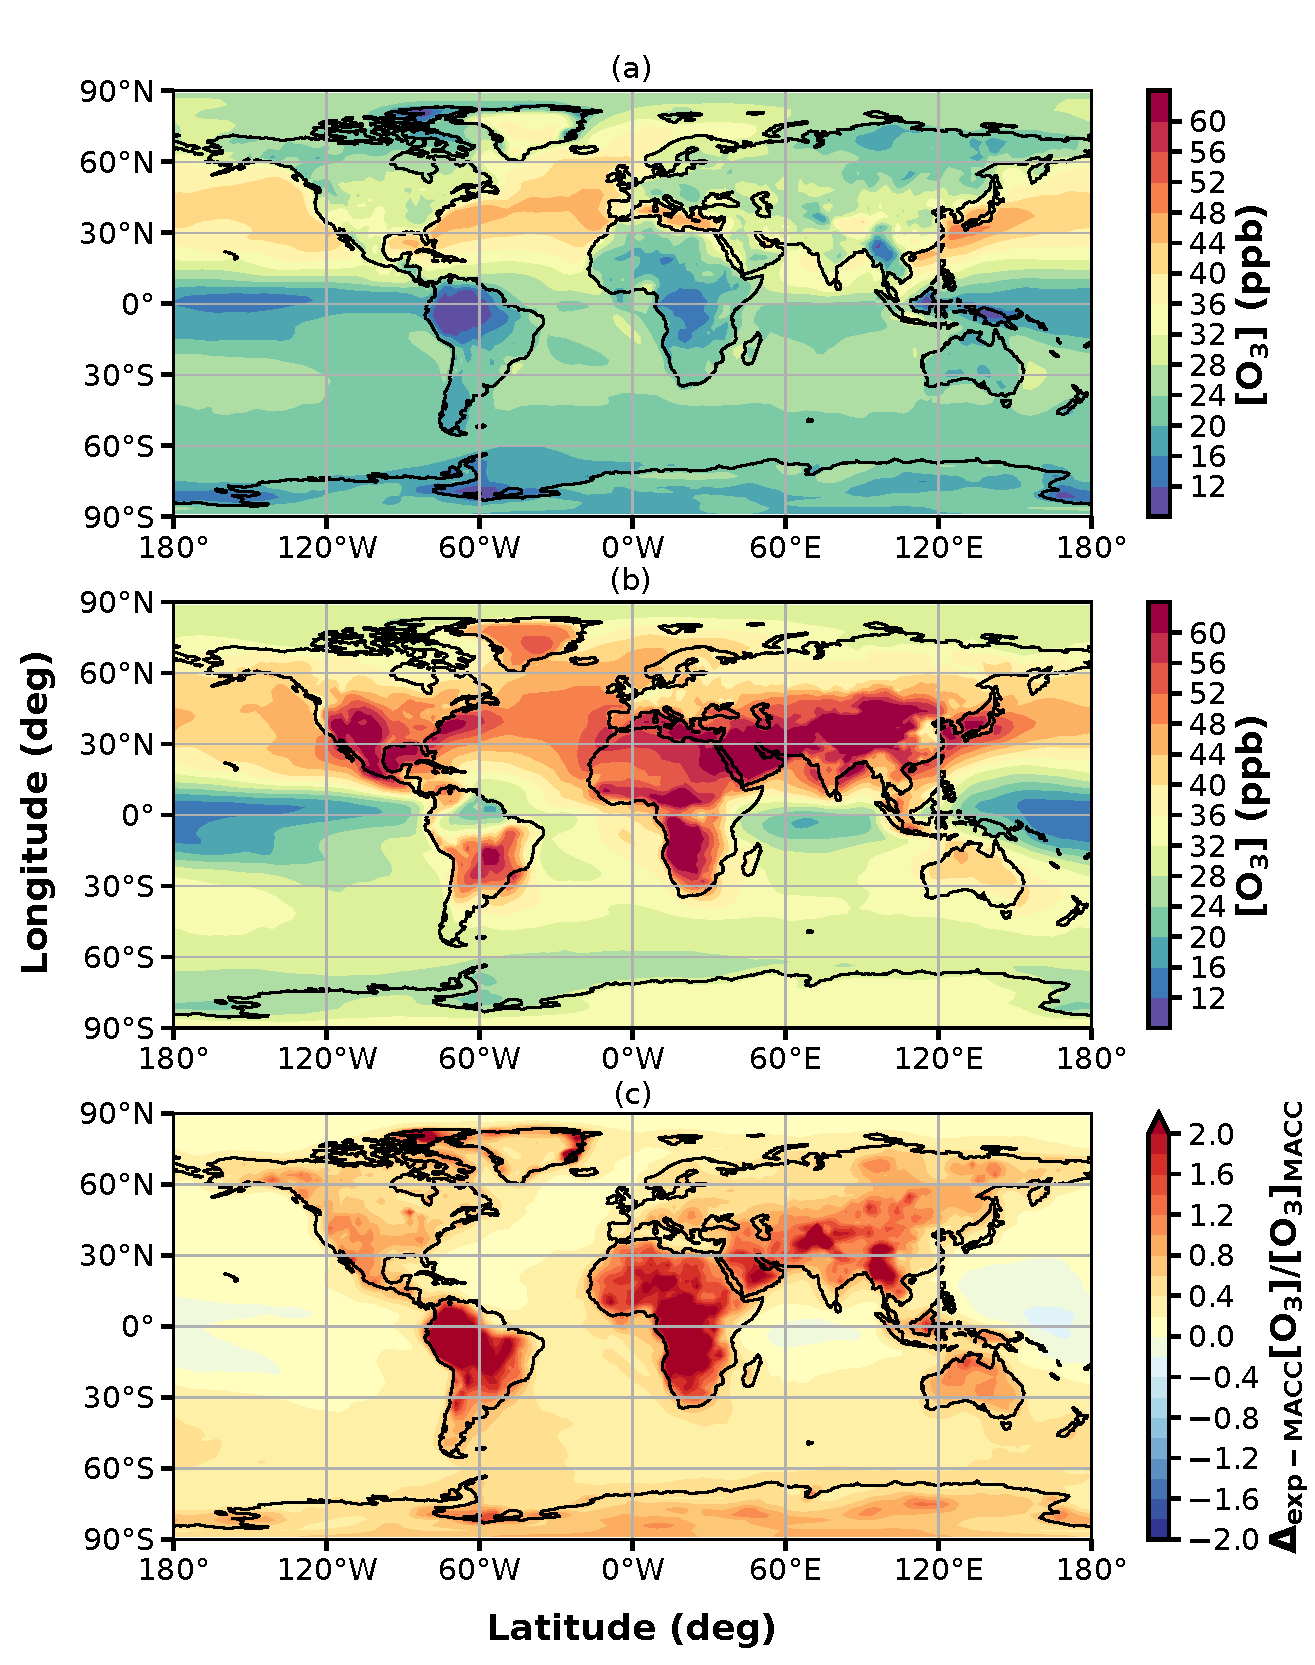
\includegraphics[width=8.3cm]{fig08}
  \caption{\DIFaddFL{Mean ozone concentrations for the year 2005. (a) MACC-reanalysis (surface); (b) Oslo~CTM3 }\emph{\DIFaddFL{mOSaic}} \DIFaddFL{(lowermost model level); (c) Relative difference.}}
  \label{fig:macc_o3conc}
\end{figure}

%DIF > %%%%%%%%%%%%%%%%%%%%%%%%%%%
\subsection{\DIFadd{Comparison with ground-based observations}}
\DIFaddend \label{subsec:obs}
In this section, we compare our \DIFaddbegin \DIFadd{model }\DIFaddend results to observations \DIFaddbegin \DIFadd{at a selected number of sites which provide ozone flux measurements}\DIFaddend . For all comparisons, we use the original resolution of the Oslo~CTM3 ($2.25^\circ\times 2.25^\circ$) instead of the re-gridded \DIFaddbegin \DIFadd{resolution }\DIFaddend ($3^\circ\times 3^\circ$).

In Fig.~\ref{fig:mmm_drydep_stations}a, seasonal cycles of average ozone dry deposition fluxes for \DIFdelbegin \DIFdel{six }\DIFdelend \DIFaddbegin \DIFadd{the six selected }\DIFaddend observation sites are shown. We have computed a model average for all sensitivity studies at the closest grid point and show the $1\,\sigma$ \DIFdelbegin \DIFdel{error }\DIFdelend \DIFaddbegin \DIFadd{uncertainty }\DIFaddend band. The shaded area around the multi-model-mean indicates the broad range of model results but is not an actual \DIFdelbegin \DIFdel{error }\DIFdelend \DIFaddbegin \DIFadd{uncertainty }\DIFaddend band since such is not given in \citet{ACP:Hardacre2015}. At \DIFdelbegin \DIFdel{about }\DIFdelend $4$ of $6$ sites, the \DIFdelbegin \DIFdel{EMEP }\DIFdelend \DIFaddbegin \DIFadd{mOSaic }\DIFaddend scheme performs better than the Wesely scheme and \DIFdelbegin \DIFdel{better than or the same as }\DIFdelend \DIFaddbegin \DIFadd{similar to or better than }\DIFaddend the multi-model-mean. We use a $\chi^2$-test
\begin{equation}
  \chi^2 = \sum_{i=1}^{12}\frac{\left(\overline{\chem{O_3}}_{\text{DD,\,}i}^\text{sim}-\overline{\chem{O_3}}_{\text{DD,\,}i}^\text{obs}\right)^2}{\sigma_i^2},
\end{equation}
with an estimated standard deviation of observation $\sigma_i=1\,\unit{mmol\,m^{-2}\,s^{-1}}$ and divide it by the number of degrees of freedom (NDF) to assess this subjective analysis in a more objective way. The closer to $1$ this test scores, the better does the simulation represent the observation. A score between $0$ and $1$ indicates that the estimated $\sigma$ is too small. The results of the $\chi^2$-test are shown together with the divergences in Fig.~\ref{fig:mmm_drydep_stations}b. The $\chi^2$-test reveals also that in $4$ of $6$ cases the \DIFdelbegin \DIFdel{EMEP }\DIFdelend \DIFaddbegin \DIFadd{mOSaic }\DIFaddend scheme improves the performance of the Oslo~CTM3 with respect to \DIFaddbegin \DIFadd{observed }\DIFaddend ozone dry deposition fluxes, although a satisfying result is only achieved for two sites (Castel Porziano, Blodgett Forest).
With only one full year of simulation, the model uncertainty regarding the seasonal cycle at observational sites cannot be properly quantified. Furthermore, the observational averages comprise at most $9$ years worth of data. Statistically, these data may still \DIFaddbegin \DIFadd{be }\DIFaddend subject to interannual variability. Among other aspects, the horizontal as well as vertical resolution play an important role in the model performance. Although, we do not explicitly assess the impacts of differing resolutions in our model, we can assume that both high and low biases exist due to dilution of sources and sinks in coarse resolution models \citep{AE:Schaap2015}. Good matches between observation and model are only to be expected if the station's location is representative for an area similar to the respective model gridbox \DIFaddbegin \DIFadd{and not substantially affected by differences in modeled and actual topography (e.g., major wind directions)}\DIFaddend .

%
\begin{figure}[t]
  \DIFdelbeginFL %DIFDELCMD < 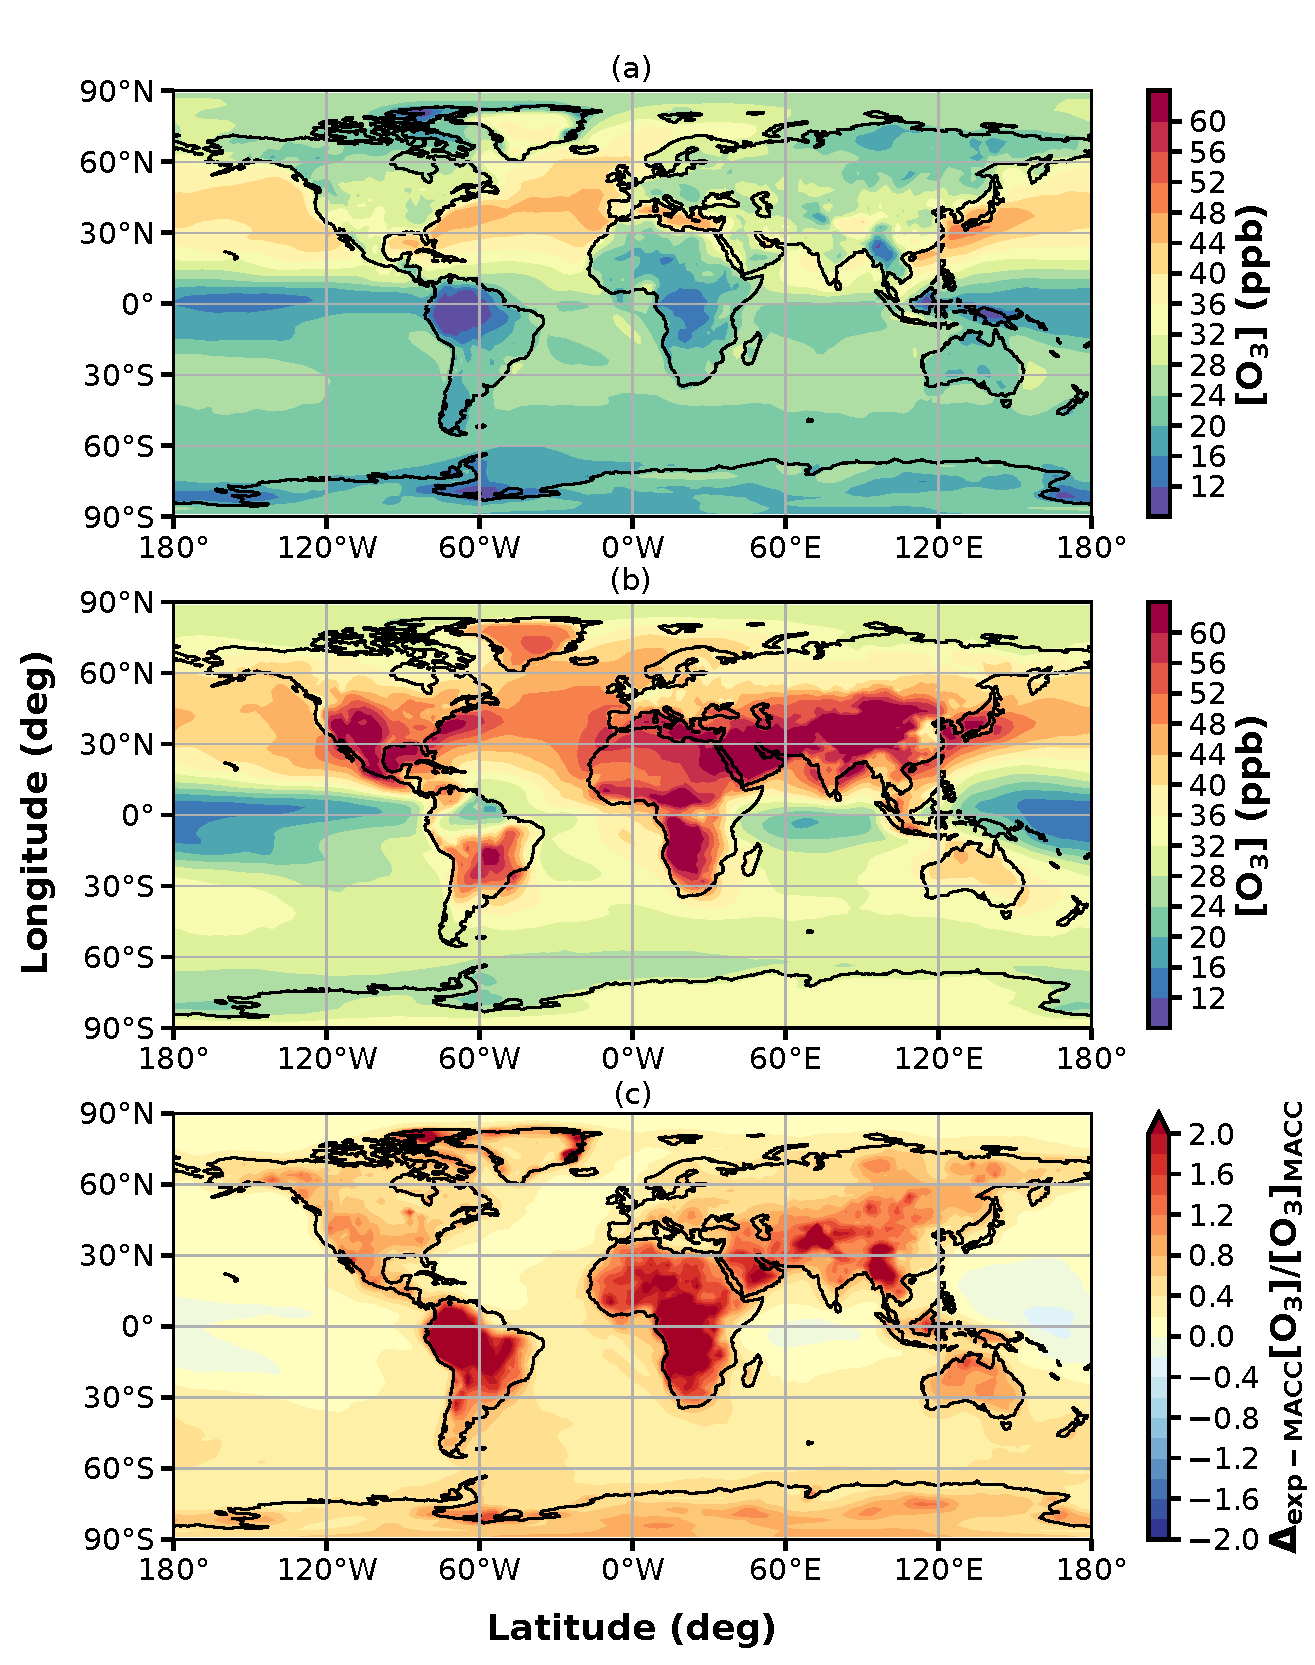
\includegraphics[width=8.3cm]{fig08}
%DIFDELCMD <   %%%
\DIFdelendFL \DIFaddbeginFL 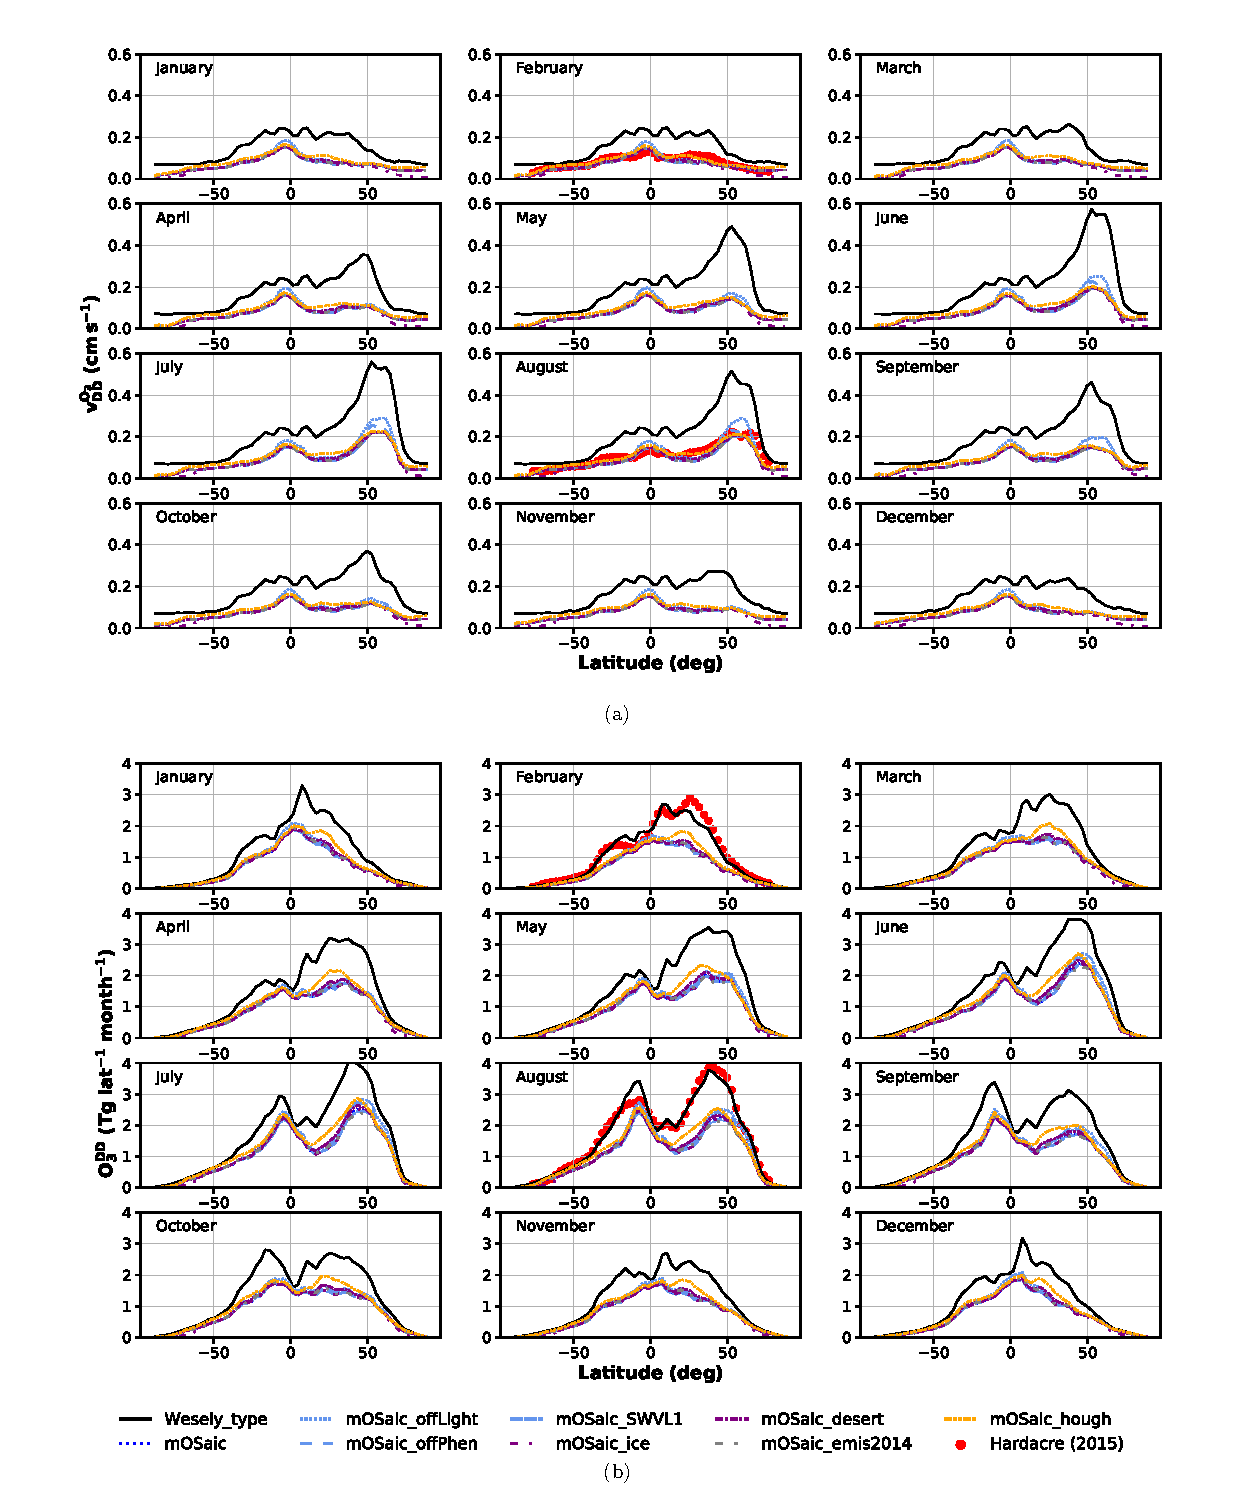
\includegraphics[width=8.3cm]{fig09}
  \DIFaddendFL \caption{Ozone dry deposition fluxes at different observation sites. (a) Comparison between Wesely scheme and average result from all sensitivity studies with observational averages taken from \citet{ACP:Hardacre2015}. The model uncertainty of the Oslo~CTM3 is given as $1\,\sigma$ error band. The shaded area around the multi-model-mean indicates the broad range of different model results but is not an actual error band. (b) Model divergence from observation and $\chi^2$-test results.}
  \label{fig:mmm_drydep_stations}
\end{figure}

%%%%%%%%%%%%%%%%%%%%%%%%%%%%
\DIFdelbegin %DIFDELCMD < \conclusions[Discussion and conclusions]  %%%
\DIFdelend \DIFaddbegin \conclusions[Summary and conclusions]  \DIFaddend %% \conclusions[modified heading if necessary]
\label{sec:conc}
We have presented an update of the dry deposition scheme in the Oslo~CTM3 from purely prescribed dry deposition velocities \citep{AE:Wesely1989,JGR:Hough1991} to a more process-oriented parameterization taking the state of the atmosphere and vegetation into account\DIFdelbegin \DIFdel{\mbox{%DIFAUXCMD
\citep{ACP:Simpson2012}}\hspace{0pt}%DIFAUXCMD
. In our implementation based on \mbox{%DIFAUXCMD
\citet{ACP:Simpson2012}}\hspace{0pt}%DIFAUXCMD
, we follow a classical, resistance analogous approach in computing }\DIFdelend \DIFaddbegin \DIFadd{. Based on the description of dry deposition in \mbox{%DIFAUXCMD
\citet{WASP:Simpson2003,ACP:Simpson2012}}\hspace{0pt}%DIFAUXCMD
, we have implemented a moasic approach to compute }\DIFaddend contributions to dry deposition \DIFdelbegin \DIFdel{. The }\DIFdelend \DIFaddbegin \DIFadd{by individual sub-grid land surface types. Aerodynamic, }\DIFaddend quasi-laminar\DIFdelbegin \DIFdel{resistance in the dry deposition scheme is capable of adjusting to surface wind stress but falls back to its prescribed limits in most of the tested cases. The surface resistance computation is }\DIFdelend \DIFaddbegin \DIFadd{, and surface resistance (latter }\DIFaddend divided into stomatal and non-stomatal \DIFdelbegin \DIFdel{resistance. The stomatal resistance is sensitive to parameters associated with the vegetation such as photosynthetic active radiation, water vapor pressure deficit, soil water content, and plant phenology, while the non-stomatal resistance is affected by the existence or absence of vegetation}\DIFdelend \DIFaddbegin \DIFadd{contributions) are calculated for each land surface category separately. Based on these, a land fraction-weighted mean is deduced. In addition, the various dry deposition velocities are now directly available from model output for diagnostics and further studies}\DIFaddend .

The \DIFaddbegin \DIFadd{new dry deposition scheme named }\emph{\DIFadd{mOSaic}} \DIFadd{improves the modeled dry deposition velocities which are now compatible with observation and model studies \mbox{%DIFAUXCMD
\citep[e.g.,][]{ACP:Hardacre2015,ACP:Luhar2018}}\hspace{0pt}%DIFAUXCMD
. Dry deposition velocities are reduced by $6-60\,\unit{\%}$. At the same time, the }\DIFaddend annual amount of ozone dry deposition decreases by \DIFdelbegin \DIFdel{up to }\DIFdelend \DIFaddbegin \DIFadd{more than }\DIFaddend $100\,\unit{\%}$ \DIFdelbegin \DIFdel{changing from the old dry deposition scheme to the new one}\DIFdelend \DIFaddbegin \DIFadd{over all major desert areas and increases over tropical forest}\DIFaddend . Compared to results from a multi-model evaluation \citep{ACP:Hardacre2015}, the total annual ozone dry deposition in the Oslo~CTM3 is \DIFdelbegin \DIFdel{about $33\,\unit{\%}$ }\DIFdelend \DIFaddbegin \DIFadd{$(38\substack{+~\,1 \\ -10})\,\unit{\%}$ }\DIFaddend below average. However, there seems to be a tendency that newer TF~HTAP models show a lower total annual dry deposition of ozone than older models, indicating that newer developments lead to decreasing ozone dry deposition and increasing tropospheric ozone burden \DIFdelbegin \DIFdel{\mbox{%DIFAUXCMD
\citep[e.g.,][]{ACP:Luhar2017,AE:Hu2017}}\hspace{0pt}%DIFAUXCMD
}\DIFdelend \DIFaddbegin \DIFadd{\mbox{%DIFAUXCMD
\citep[e.g.,][]{ACP:Luhar2017,ACP:Luhar2018,AE:Hu2017}}\hspace{0pt}%DIFAUXCMD
}\DIFaddend .

We found the response of the Oslo~CTM3 to the changes in dry deposition velocities from the old and the \DIFdelbegin \DIFdel{new dry deposition }\DIFdelend \DIFaddbegin \DIFadd{mOSaic }\DIFaddend scheme to be consistent. A decrease in $v_\text{DD}^\chem{O_3}$ leads to a decrease in total ozone dry deposition and an increase in \DIFdelbegin \DIFdel{surface ozone concentration $[\chem{O_3}(z_0)]$}\DIFdelend \DIFaddbegin \DIFadd{ozone concentration $[\chem{O_3}]$}\DIFaddend . As the new scheme is \DIFaddbegin \DIFadd{quantitatively }\DIFaddend more similar to the multi-model-mean \citep{ACP:Hardacre2015} with respect to dry deposition velocities, while the old scheme agrees better in terms of total dry deposition, there is an apparent discrepancy\DIFdelbegin \DIFdel{when comparing with the multi-model-mean. Without knowing $[\chem{O_3}(z_0)]$ of the TF~HTAP models, this cannot be }\DIFdelend \DIFaddbegin \DIFadd{. By means of tropospheric ozone burden \mbox{%DIFAUXCMD
\citep{ESA:Gaudel2018} }\hspace{0pt}%DIFAUXCMD
and surface ozone concentrations deduced from the MACC-reanalysis \mbox{%DIFAUXCMD
\citep{MACC-II}}\hspace{0pt}%DIFAUXCMD
, the Oslo~CTM3 with operational mOSaic scheme shows a pronounced high-bias of tropospheric ozone. While the average bias is small or even reversed when using the old scheme, both display elevated ozone in comparison with the MACC-reanalysis in continental regions with high average incoming UV radiation (e.g., northern South America, central and southern Africa, the Himalayas).
The reason behind this bias has not yet been }\DIFaddend resolved and may hint to, e.g., \DIFdelbegin \DIFdel{differences }\DIFdelend \DIFaddbegin \DIFadd{issues }\DIFaddend in photo-chemistry \DIFdelbegin \DIFdel{, stratosphere-troposphere-exchange as well as to differences in aerosol loadings among many other aspects}\DIFdelend \DIFaddbegin \DIFadd{($[\chem{OH}]$ related ozone production and loss) or previously introduced optimization of ozone removal with respect to the old, less physical dry deposition velocities}\DIFaddend .

Most of the \DIFdelbegin \DIFdel{decrease }\DIFdelend \DIFaddbegin \DIFadd{qualitative change }\DIFaddend in ozone dry deposition in the Oslo~CTM3 \DIFaddbegin \DIFadd{($-2-12\,\unit{\%}$) }\DIFaddend can be attributed to changes in dry deposition \DIFdelbegin \DIFdel{velocities }\DIFdelend over the ocean and deserts. This is mainly due to updates of the respective\DIFdelbegin \DIFdel{prescribed dry deposition velocities $v_\text{DD}^\chem{O_3}$}\DIFdelend \DIFaddbegin \DIFadd{, prescribed ozone surface resistances $R^\chem{O_3}$}\DIFaddend . In case of desert and grasslands the difference between the old and new prescribed value is \DIFdelbegin \DIFdel{at }\DIFdelend \DIFaddbegin \DIFadd{in }\DIFaddend the order of $1$ magnitude. Over the ocean, the absolute change in dry deposition is small, but it is accumulated over a large area which is especially amplified in the southern hemisphere. Small adjustments to the lower limits in our quasi-laminar layer resistance formulation may help improve the Oslo~CTM3 performance in this regard. With respect to available measurements of dry deposition velocities of ozone over desert \citep{AE:Gusten1995} and ocean \citep{JGR:Helmig2012}, the new Oslo~CTM3 dry deposition scheme slightly underestimates ozone dry deposition velocities over the former and overestimate them over the latter. Regarding the vastness of the ocean and the ongoing desertification, it may be worthwhile to \DIFdelbegin \DIFdel{study dry deposition in these regimes at a }\DIFdelend \DIFaddbegin \DIFadd{revise the dry deposition scheme for these regimes and add }\DIFaddend more process-oriented \DIFdelbegin \DIFdel{level}\DIFdelend \DIFaddbegin \DIFadd{formulations}\DIFaddend , e.g., 2-layer gas exchange with ocean waters \DIFdelbegin \DIFdel{\mbox{%DIFAUXCMD
\citep{ACP:Luhar2017}}\hspace{0pt}%DIFAUXCMD
}\DIFdelend \DIFaddbegin \DIFadd{\mbox{%DIFAUXCMD
\citep{ACP:Luhar2017, ACP:Luhar2018}}\hspace{0pt}%DIFAUXCMD
}\DIFaddend , wave braking and spray \citep{ACP:Pozzer2006}.

Although dry deposition to ice and snow amounts to \DIFdelbegin \DIFdel{less than }\DIFdelend \DIFaddbegin \DIFadd{only }\DIFaddend $1\,\unit{\%}$ of the total global annual ozone dry deposition \DIFaddbegin \DIFadd{in }\emph{\DIFadd{mOSaic}}\DIFaddend , a decrease in prescribed dry deposition velocity in accordance to combined measurements and model studies \citep{ACP:Helmig2007} causes almost a doubling in the surface ozone concentrations in the high Arctics and affects surface ozone concentrations down to latitudes at \DIFdelbegin \DIFdel{about }\DIFdelend $50\,\unit{^\circ}$ in both hemispheres. \DIFdelbegin \DIFdel{By comparing }\DIFdelend \DIFaddbegin \DIFadd{Comparing }\DIFaddend with results from the multi-model evaluation \citep{ACP:Hardacre2015}, we conclude that it is important to use this updated ozone dry deposition velocity to counter an Arctic surface ozone low-bias in \DIFdelbegin \DIFdel{the model}\DIFdelend \DIFaddbegin \DIFadd{models}\DIFaddend , however, this \DIFdelbegin \DIFdel{could lead }\DIFdelend \DIFaddbegin \DIFadd{currently leads }\DIFaddend to an overcompensation (high-bias) \DIFaddbegin \DIFadd{in the Oslo~CTM3}\DIFaddend .

We have studied the parameter space of the stomatal conductance parameterization and found that total surface ozone in the tropics \DIFaddbegin \DIFadd{and the northern hemisphere }\DIFaddend is most sensitive to changes \DIFdelbegin \DIFdel{in ozone uptake by plants. The difference between our }\DIFdelend \DIFaddbegin \DIFadd{therein. In the }\DIFaddend most extreme test \DIFdelbegin \DIFdel{cases amounts to $15\,\unit{\%}$ with respect to total surface ozone}\DIFdelend \DIFaddbegin \DIFadd{case, the increase in global total dry deposition amounts to $7.3\,\unit{\%}$}\DIFaddend , while the more realistic test \DIFdelbegin \DIFdel{case }\DIFdelend \DIFaddbegin \DIFadd{cases, e.g. }\DIFaddend using differing years of emission \DIFdelbegin \DIFdel{amounts to about $5\,\unit{\%}$}\DIFdelend \DIFaddbegin \DIFadd{amount to changes in the order of $\pm 2\,\unit{\%}$}\DIFaddend . This may indicate that future changes in vegetation cover and solar radiation at the surface due to changes in stratospheric ozone, cloud cover, or aerosols could also strongly influence the surface ozone burden in the tropics. Total column ozone in the tropics is predicted to decrease due to changes in the atmospheric circulation \citep[e.g.,][]{WMO2014}, while tropospheric and surface ozone increase. The combined effects of increasing emissions of ozone precursors and an increase in UV due to thinning of stratospheric ozone might permit more UV light at ground and thus increase the ozone production.

\DIFdelbegin \DIFdel{In the northern hemisphere mid and high latitudes ($50\,\unit{^\circ}-75\,\unit{^\circ N}$), total surface ozone increases by about $7.7\,\unit{\%}$ if the beginning and end of the vegetation period is estimated based on a $5\,\unit{^\circ C}$-days criteria instead of prescribed. This is very important for any study focusing on ozone in the boreal and subarctic regions.
}\DIFdelend %DIF > In the northern hemisphere mid and high latitudes ($50\,\unit{^\circ}-75\,\unit{^\circ N}$), total surface ozone increases by $7.7\,\unit{\%}$ if the beginning and end of the vegetation period is estimated based on a $5\,\unit{^\circ C}$-days criteria instead of prescribed. This is very important for any study focusing on ozone in the boreal and subarctic regions.

An important factor in the global ozone budget are emissions of precursor substances. We cover this by using the same meteorology with different years of CEDS emissions. We chose the years 2005 and 2014 for our comparison. \DIFaddbegin \DIFadd{Ozone precursor emissions in 2014 are slightly lower in the NH while enhanced in the tropics and the SH. }\DIFaddend In 2014, surface ozone burden is higher in the southern hemisphere and in the tropics (\DIFdelbegin \DIFdel{$\sim 5\,\unit{\%}$}\DIFdelend \DIFaddbegin \DIFadd{$5\,\unit{\%}$}\DIFaddend ) compared to 2005, while it is lower in the northern hemisphere (\DIFdelbegin \DIFdel{$\sim 2\,\unit{\%}$).
This is most likely reflecting the ongoing industrialization process of countries in the southern hemisphere and the commitment and implementation of air quality regulations of industrialized nations in the northern hemisphere.
}\DIFdelend \DIFaddbegin \DIFadd{$2\,\unit{\%}$).
}\DIFaddend 

We also evaluated the model with respect to observed dry deposition \DIFdelbegin \DIFdel{velocities }\DIFdelend \DIFaddbegin \DIFadd{fluxes }\DIFaddend at six sites in the northern hemisphere and found that the \DIFdelbegin \DIFdel{updated dry deposition }\DIFdelend \DIFaddbegin \DIFadd{mOSaic }\DIFaddend scheme performs better than the old one, but is not able to reproduce the measurements at most sites quantitatively. This may be due to several reasons. The model resolution in both horizontal ($2.25^\circ\times 2.25^\circ$) and vertical (L60, $P_\text{max}=0.02\,\unit{hPa}$) does not capture all details in transport, thus affecting the distribution and transport (e.g., long-range, convection, and stratosphere--troposphere exchange) of ozone and its precursors. Depending on the location of the observation site and its respective representativeness for a larger area, ozone dry deposition and ozone concentrations are expected to be over- or underestimated in the model. \DIFaddbegin \DIFadd{Because of non-linearities in ozone formation and destruction, ozone concentrations are sensitive to both, differences in local concentration of precursors and meteorological conditions \mbox{%DIFAUXCMD
\citep{JGR:Jin2013}}\hspace{0pt}%DIFAUXCMD
. }\DIFaddend In addition, a comparison of very few years of measurement to only one specific year of simulation may reflect the year to year variability more than the actual model performance.

Future work on the Oslo~CTM3 should \DIFdelbegin \DIFdel{include a direct output of dry deposition velocities for diagnostic purposes. The }\DIFdelend \DIFaddbegin \DIFadd{resolve the ozone high-bias which may involve revising the photolysis- and chemical reaction computation as well as reaction rates. For a better modeling of ozone abundances, ocean emissions of very short-lived ozone depleting substances (VSLS) \mbox{%DIFAUXCMD
\citep{JGR:Warwick2006, ACP:Ziska2013} }\hspace{0pt}%DIFAUXCMD
which affect the stratospheric ozone \mbox{%DIFAUXCMD
\citep{ACP:Hossaini2016, ACP:Falk2017} }\hspace{0pt}%DIFAUXCMD
and a scheme covering arctic spring-time ozone depletion \mbox{%DIFAUXCMD
\citep[e.g.,][]{ACP:Yang2010, ACP:Toyota2011, GMD:Falk2018}}\hspace{0pt}%DIFAUXCMD
, could be worthwhile implementing. The general }\DIFaddend model performance could also be improved by allowing for more plant functional types and phenologies than currently used or implementing an actual photosynthesis-based modeling of plants. \DIFdelbegin \DIFdel{The photolysis- and chemical reaction computation as well as reaction rates shall also be revised in the future}\DIFdelend \DIFaddbegin \DIFadd{A more efficient parallelization of the code would enable computation on higher horizontal resolutions}\DIFaddend .

%% The following commands are for the statements about the availability of data sets and/or software code corresponding to the manuscript.
%% It is strongly recommended to make use of these sections in case data sets and/or software code have been part of your research the article is based on.

%\codeavailability{TEXT} %% use this section when having only software code available


%\dataavailability{TEXT} %% use this section when having only data sets available


\DIFdelbegin %DIFDELCMD < \codedataavailability{The Oslo~CTM3 is publicly available on git-hub under a MIT license. Model results can be made available under request.} %%%
\DIFdelend \DIFaddbegin \codedataavailability{The Oslo~CTM3 shall be publicly available on git-hub under a MIT license in the future. Until then, access can be made granted under request. Model results can be made available under request.} \DIFaddend %% use this section when having data sets and software code available


%\sampleavailability{TEXT} %% use this section when having geoscientific samples available
%\videosupplement{TEXT} %% use this section when having video supplements available


%\clearpage

\appendix
\section{Figures}    %% Appendix A

\appendixfigures
\begin{figure}[!htbp]
  \DIFdelbeginFL %DIFDELCMD < 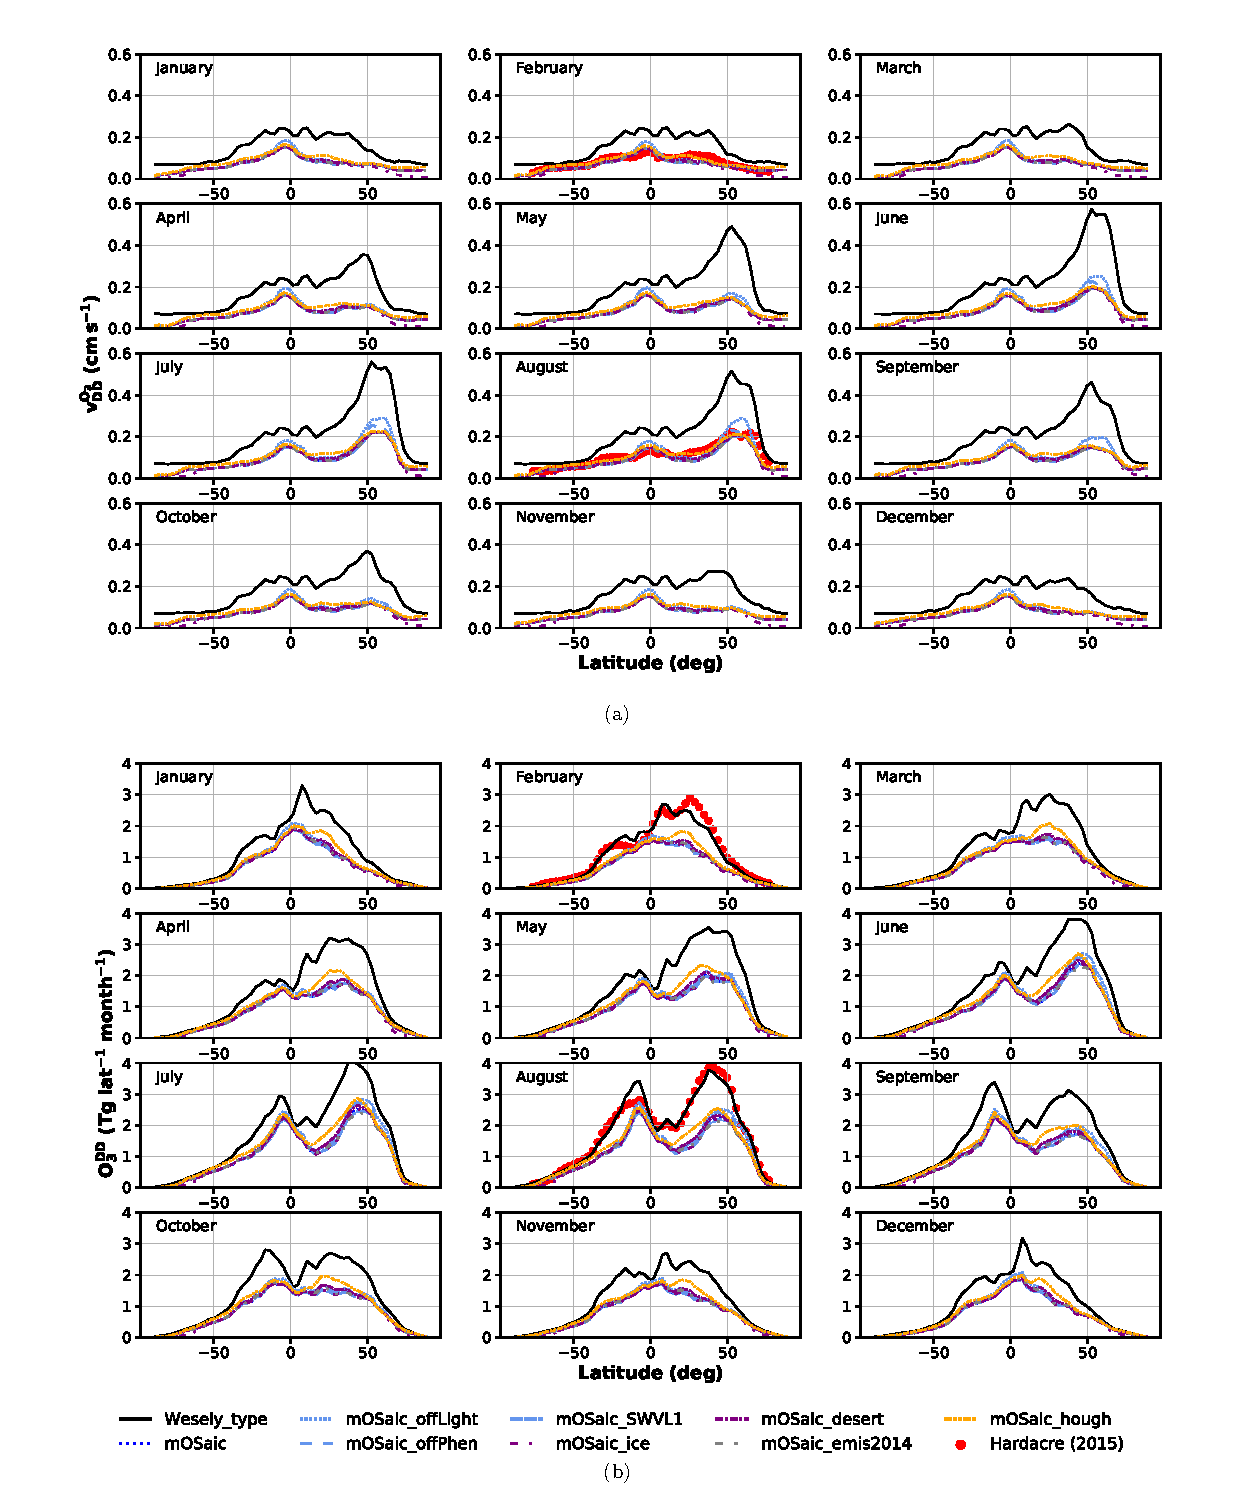
\includegraphics[width=0.8\textwidth]{fig09}
%DIFDELCMD <   %%%
\DIFdelendFL \DIFaddbeginFL 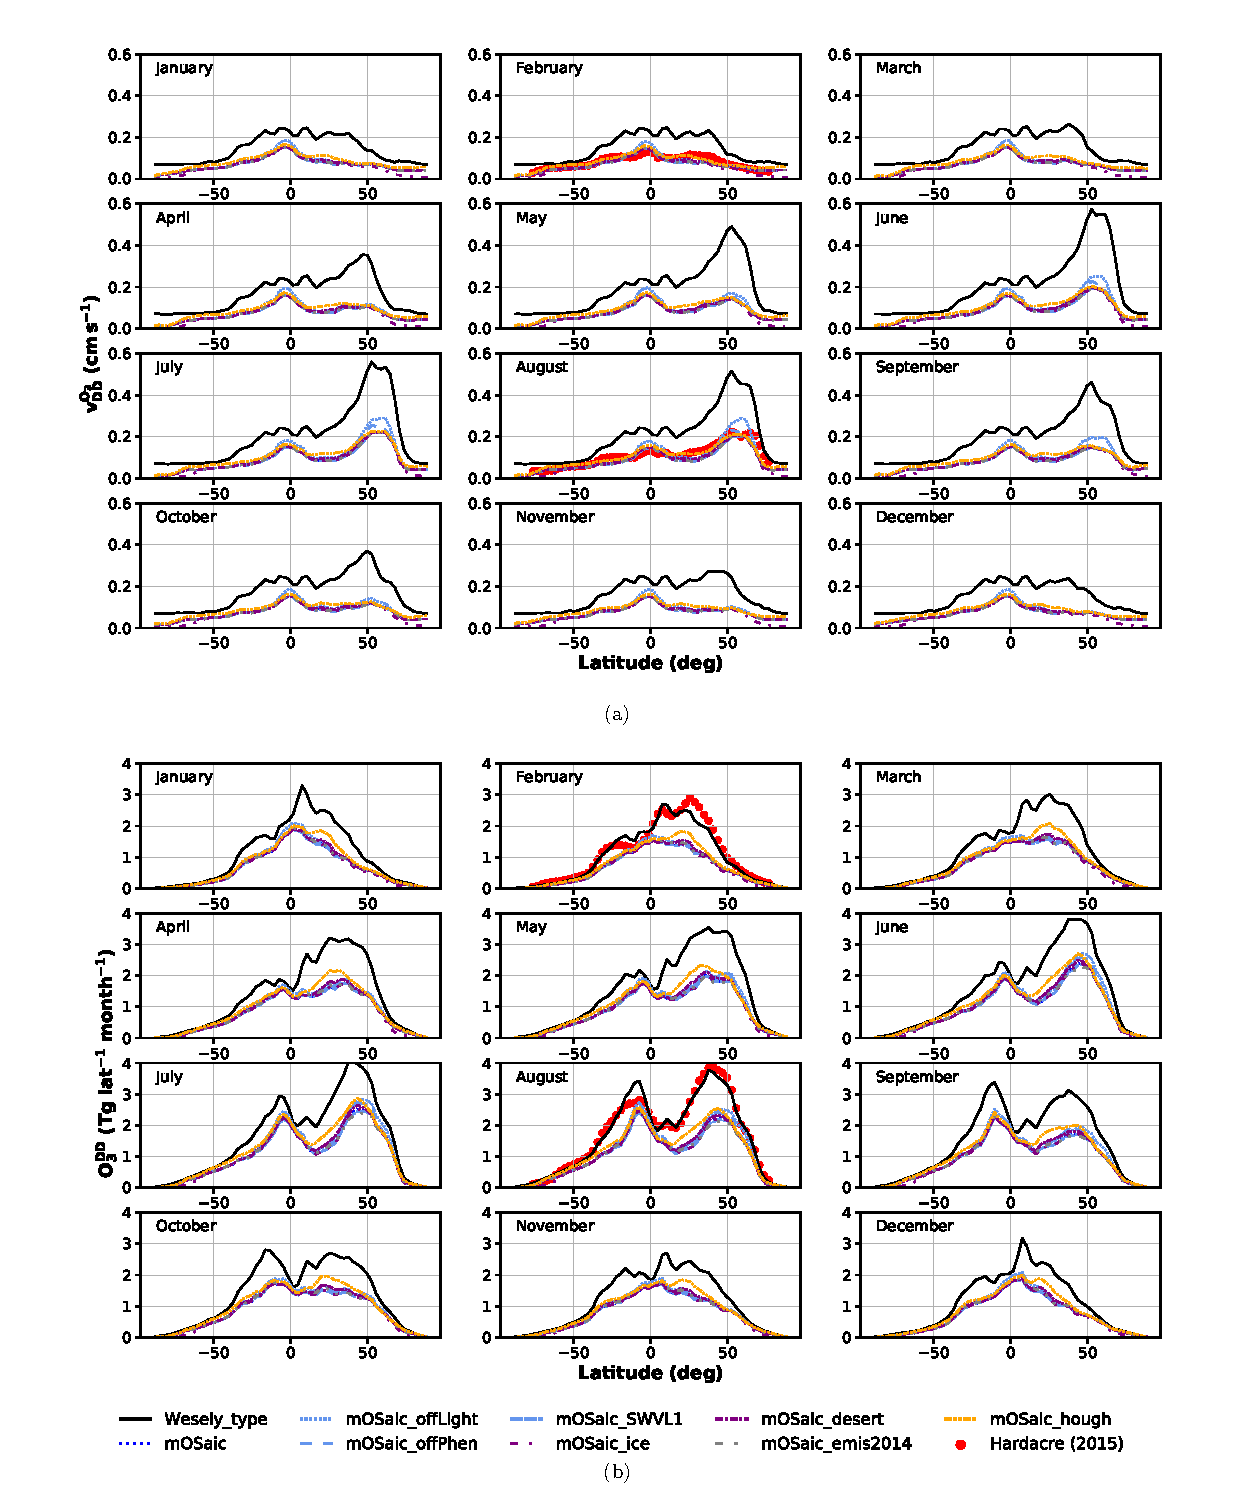
\includegraphics[width=0.8\textwidth]{fig10}
  \DIFaddendFL \caption{Comparison of the manifold of Oslo~CTM3 integrations with respect to (a) Zonal average ozone dry deposition velocities; (b) Total annual amount of ozone removed from the atmosphere via dry deposition. The multi-model mean from the evaluation of TF~HTAP models by \citet{ACP:Hardacre2015} is shown as a reference (where available).}
  \label{fig:mmm_drydep_season}
\end{figure}

\appendixfigures
\begin{figure*}[!htbp]
  \centering
  \DIFdelbeginFL %DIFDELCMD < 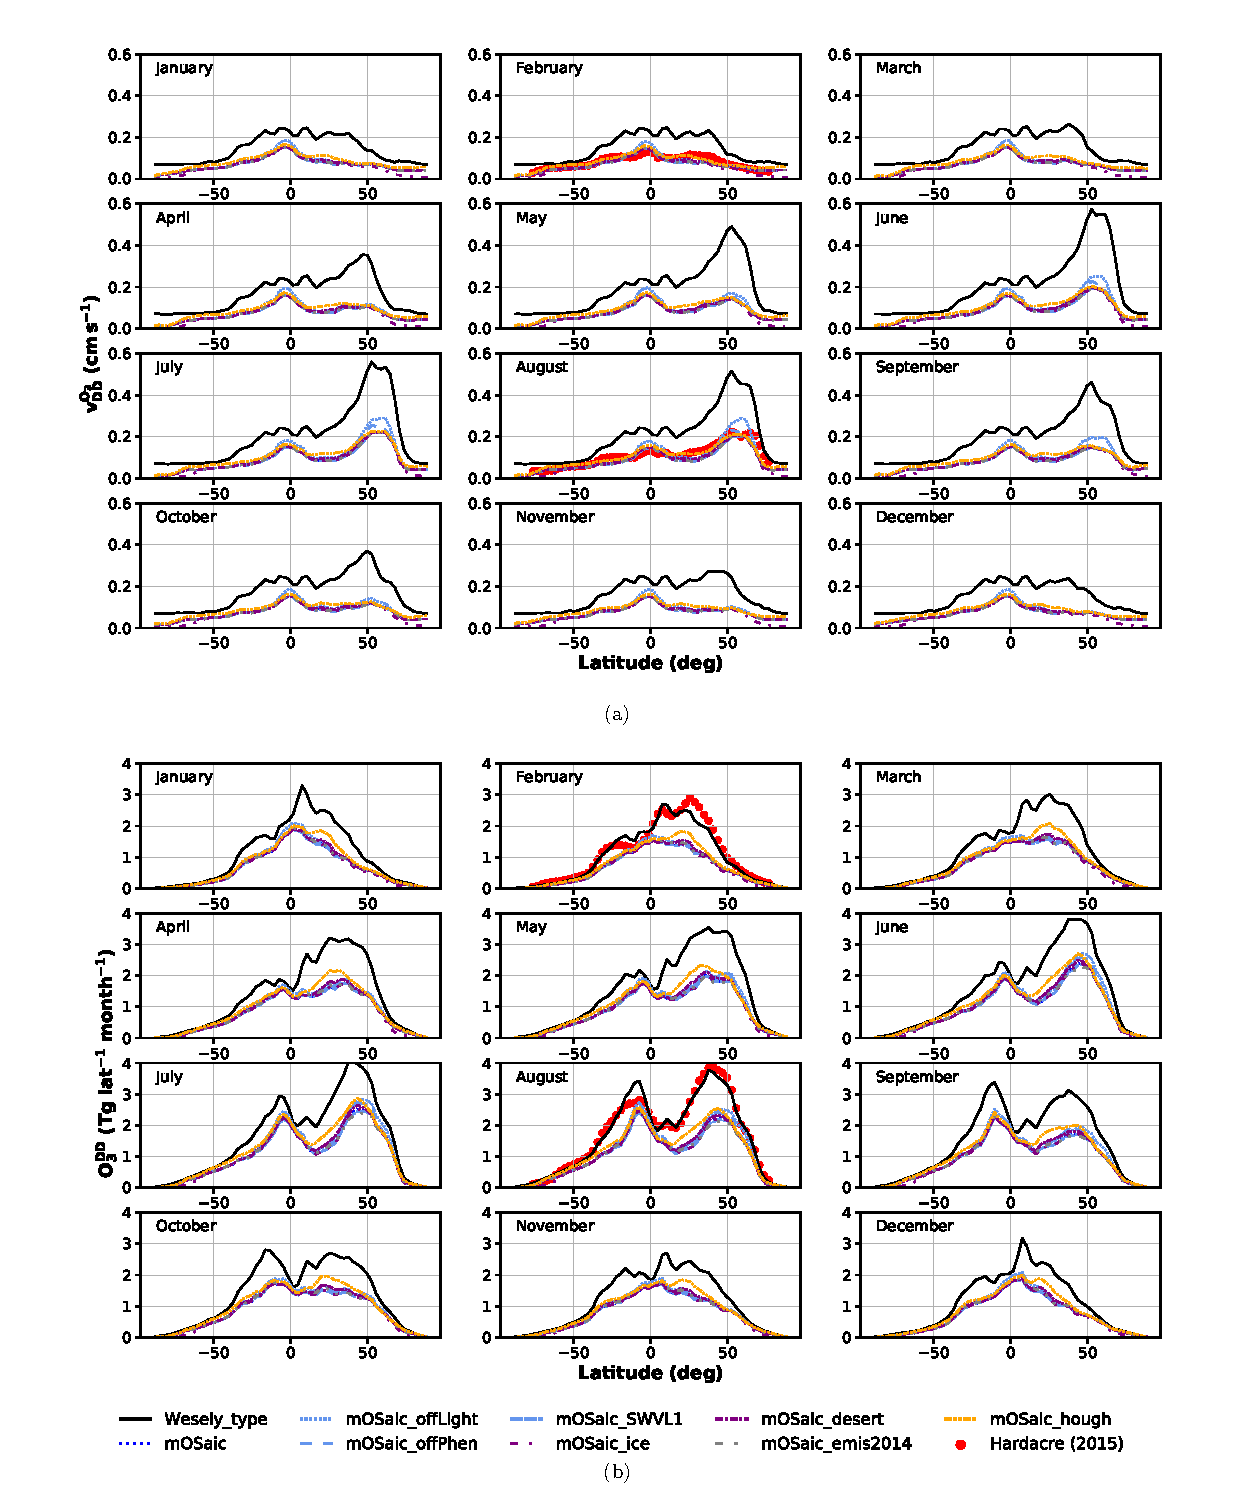
\includegraphics[width=0.8\textwidth]{fig10}
%DIFDELCMD <   %%%
\DIFdelendFL \DIFaddbeginFL 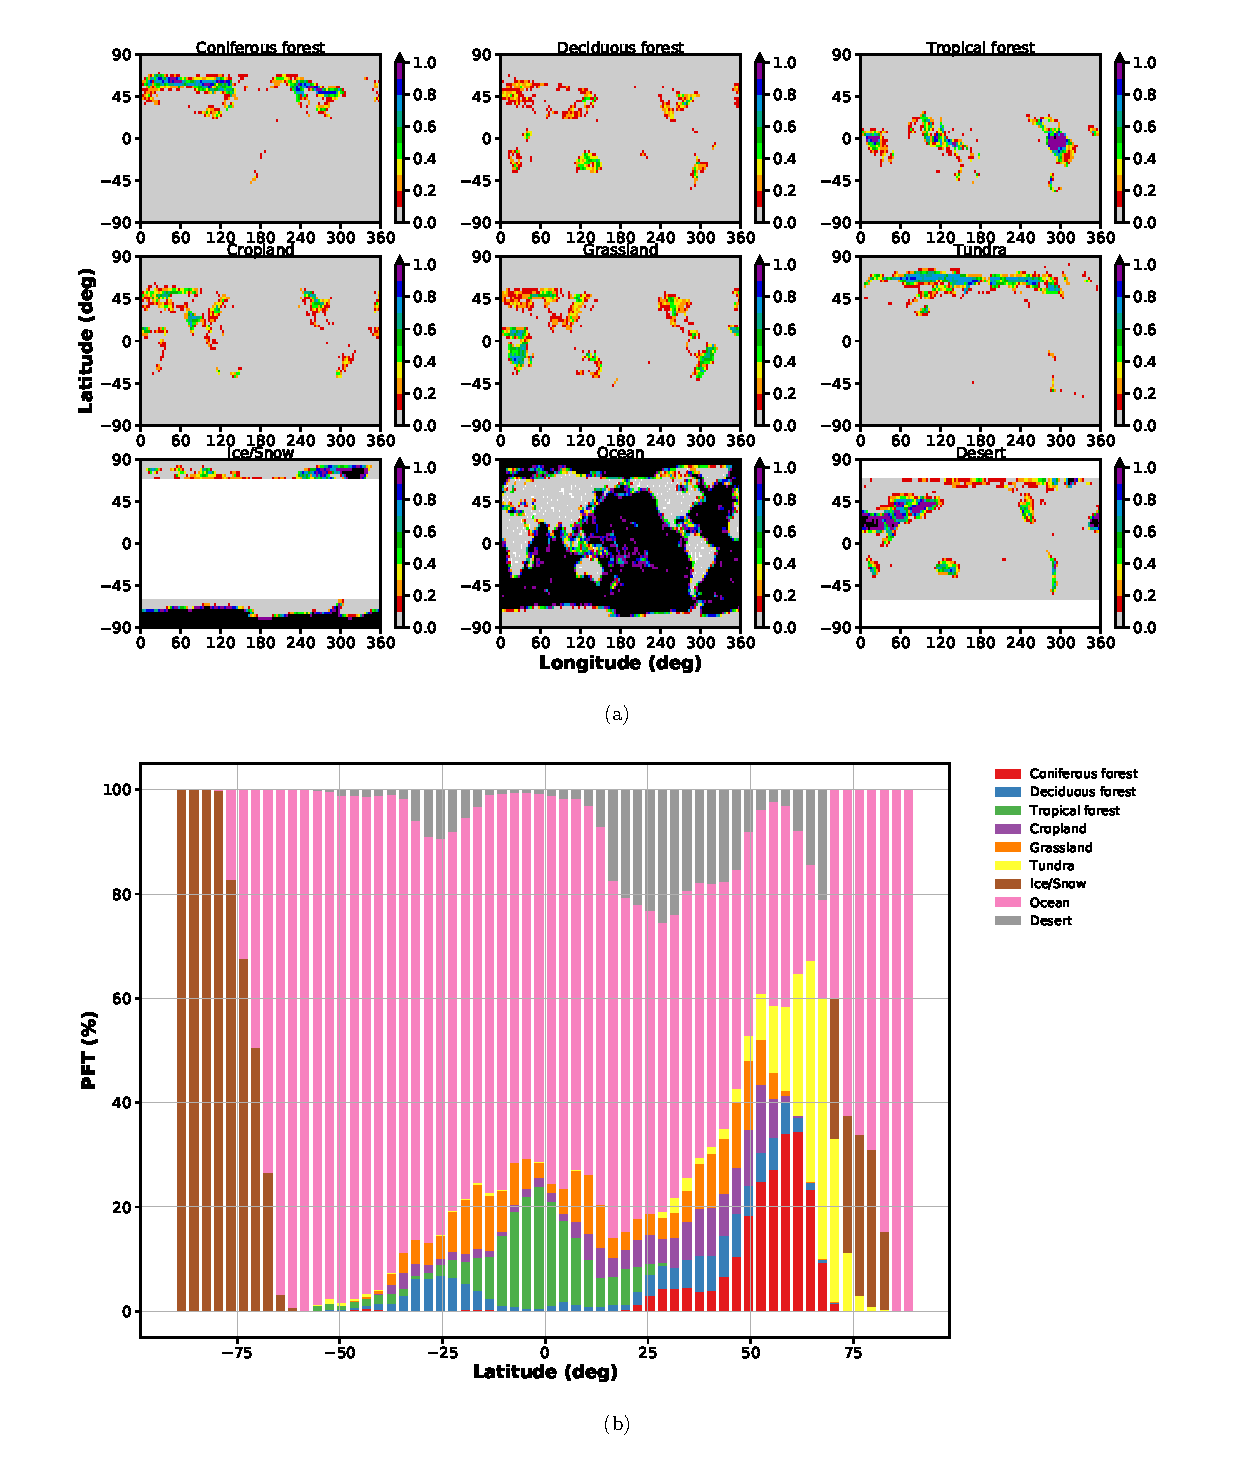
\includegraphics[width=0.8\textwidth]{fig11}
  \DIFaddendFL \caption{Partitioning of land surface types. (a) CLM~2 dynamic land surface types in $(0.5\times0.5)\,\unit{^\circ}$ resolution; (b) Zonal distribution of land surface types.}
  \label{fig:pft_landsurface}
\end{figure*}

%\subsection{}     %% Appendix A1, A2, etc.


\noappendix       %% use this to mark the end of the appendix section

%% Regarding figures and tables in appendices, the following two options are possible depending on your general handling of figures and tables in the manuscript environment:

%% Option 1: If you sorted all figures and tables into the sections of the text, please also sort the appendix figures and appendix tables into the respective appendix sections.
%% They will be correctly named automatically.

%% Option 2: If you put all figures after the reference list, please insert appendix tables and figures after the normal tables and figures.
%% To rename them correctly to A1, A2, etc., please add the following commands in front of them:

%\appendixfigures  %% needs to be added in front of appendix figures

%\appendixtables   %% needs to be added in front of appendix tables

%% Please add \clearpage between each table and/or figure. Further guidelines on figures and tables can be found below.



\DIFdelbegin %DIFDELCMD < \authorcontribution{Stefanie Falk has compiled the manuscript, finalized the implementation of the stomatal conductance in the EMEP-based dry deposition scheme of the Oslo~CTM3, conducted the simulations, and analysed and evaluated the results. Amund S{\o}vde Haslerud has implemented the EMEP-based dry deposition scheme and wrote the respective documentation. Both authors contributed to the writing and discussion of the paper.} %%%
\DIFdelend \DIFaddbegin \authorcontribution{Stefanie Falk has compiled the manuscript, finalized the implementation of the stomatal conductance in the EMEP-based dry deposition scheme of the Oslo~CTM3, conducted the simulations, and analyzed and evaluated the results. Amund S{\o}vde Haslerud has implemented the EMEP-based dry deposition scheme and wrote the respective documentation. Both authors contributed to the writing and discussion of the paper.} \DIFaddend %% this section is mandatory for the journals ACP and GMD. For all other journals it is strongly recommended to make use of this section

\competinginterests{The authors declare that they have no conflict of interest.} %% this section is mandatory even if you declare that no competing interests are present

%\disclaimer{TEXT} %% optional section

\begin{acknowledgements}
  This work was supported by the Norwegian Research Council (NRC) through the project The double punch: Ozone and climate stresses on vegetation (268073).\\
  The simulations were performed on resources provided by UNINETT Sigma2 -- the National Infrastructure for High Performance Computing and Data Storage in Norway (project nn2806k).\\
  The used Leaf Area Index (LAI) and roughness length ($z_0$) are available online from Oak Ridge National Laboratory Distributed Active Archive Center, Oak Ridge, Tennessee, U.S.A. (\doi{10.3334/ORNLDAAC/970}).\\
  Community Emission Data System (CEDS) historical emission inventory is provided by the Joint Global Research Institute project (\url{http://www.globalchange.umd.edu/ceds/}.)
  Randerson, J.T., G.R. van der Werf, L. Giglio, G.J. Collatz, and P.S. Kasibhatla. 2018. Global Fire Emissions Database, Version 4, (GFEDv4). ORNL DAAC, Oak Ridge, Tennessee, USA. https://doi.org/10.3334/ORNLDAAC/1293
  We would like to thank Prof. Frode Stordal (Section for Meteorology and Oceanography, University of Oslo) for discussions regarding early drafts of the manuscript\DIFdelbegin \DIFdel{as well as }\DIFdelend \DIFaddbegin \DIFadd{, }\DIFaddend Anne Fouilloux (scientific programmer at the same institute) for technical support \DIFaddbegin \DIFadd{as well as Olimpia Bruno (Karlsruhe Institute of Technology) and Franziska Hellmuth (University of Oslo) for valuable input regarding the aerodynamic resistance formulation}\DIFaddend .
  We would also like to thank the Center for International Climate Research (CICERO) for their support of this work.
\end{acknowledgements}




%% REFERENCES

%% The reference list is compiled as follows:

%% Since the Copernicus LaTeX package includes the BibTeX style file copernicus.bst,
%% authors experienced with BibTeX only have to include the following two lines:
%%
\bibliographystyle{copernicus}
\bibliography{DryDep.bib}
%%
%% URLs and DOIs can be entered in your BibTeX file as:
%%
%% URL = {http://www.xyz.org/~jones/idx_g.htm}
%% DOI = {10.5194/xyz}


%% LITERATURE CITATIONS
%%
%% command                        & example result
%% \citet{jones90}|               & Jones et al. (1990)
%% \citep{jones90}|               & (Jones et al., 1990)
%% \citep{jones90,jones93}|       & (Jones et al., 1990, 1993)
%% \citep[p.~32]{jones90}|        & (Jones et al., 1990, p.~32)
%% \citep[e.g.,][]{jones90}|      & (e.g., Jones et al., 1990)
%% \citep[e.g.,][p.~32]{jones90}| & (e.g., Jones et al., 1990, p.~32)
%% \citeauthor{jones90}|          & Jones et al.
%% \citeyear{jones90}|            & 1990



%% FIGURES

%% When figures and tables are placed at the end of the MS (article in one-column style), please add \clearpage
%% between bibliography and first table and/or figure as well as between each table and/or figure.


%% ONE-COLUMN FIGURES

%%f
%\begin{figure}[t]
%\includegraphics[width=8.3cm]{FILE NAME}
%\caption{TEXT}
%\end{figure}
%
%%% TWO-COLUMN FIGURES
%
%%f
%\begin{figure*}[t]
%\includegraphics[width=12cm]{FILE NAME}
%\caption{TEXT}
%\end{figure*}
%
%
%%% TABLES
%%%
%%% The different columns must be seperated with a & command and should
%%% end with \\ to identify the column brake.
%
%%% ONE-COLUMN TABLE
%
%%t
%\begin{table}[t]
%\caption{TEXT}
%\begin{tabular}{column = lcr}
%\tophline
%
%\middlehline
%
%\bottomhline
%\end{tabular}
%\belowtable{} % Table Footnotes
%\end{table}
%
%%% TWO-COLUMN TABLE
%
%%t
%\begin{table*}[t]
%\caption{TEXT}
%\begin{tabular}{column = lcr}
%\tophline
%
%\middlehline
%
%\bottomhline
%\end{tabular}
%\belowtable{} % Table Footnotes
%\end{table*}
%
%%% LANDSCAPE TABLE
%
%%t
%\begin{sidewaystable*}[t]
%\caption{TEXT}
%\begin{tabular}{column = lcr}
%\tophline
%
%\middlehline
%
%\bottomhline
%\end{tabular}
%\belowtable{} % Table Footnotes
%\end{sidewaystable*}
%
%
%%% MATHEMATICAL EXPRESSIONS
%
%%% All papers typeset by Copernicus Publications follow the math typesetting regulations
%%% given by the IUPAC Green Book (IUPAC: Quantities, Units and Symbols in Physical Chemistry,
%%% 2nd Edn., Blackwell Science, available at: http://old.iupac.org/publications/books/gbook/green_book_2ed.pdf, 1993).
%%%
%%% Physical quantities/variables are typeset in italic font (t for time, T for Temperature)
%%% Indices which are not defined are typeset in italic font (x, y, z, a, b, c)
%%% Items/objects which are defined are typeset in roman font (Car A, Car B)
%%% Descriptions/specifications which are defined by itself are typeset in roman font (abs, rel, ref, tot, net, ice)
%%% Abbreviations from 2 letters are typeset in roman font (RH, LAI)
%%% Vectors are identified in bold italic font using \vec{x}
%%% Matrices are identified in bold roman font
%%% Multiplication signs are typeset using the LaTeX commands \times (for vector products, grids, and exponential notations) or \cdot
%%% The character * should not be applied as mutliplication sign
%
%
%%% EQUATIONS
%
%%% Single-row equation
%
%\begin{equation}
%
%\end{equation}
%
%%% Multiline equation
%
%\begin{align}
%& 3 + 5 = 8\\
%& 3 + 5 = 8\\
%& 3 + 5 = 8
%\end{align}
%
%
%%% MATRICES
%
%\begin{matrix}
%x & y & z\\
%x & y & z\\
%x & y & z\\
%\end{matrix}
%
%
%%% ALGORITHM
%
%\begin{algorithm}
%\caption{...}
%\label{a1}
%\begin{algorithmic}
%...
%\end{algorithmic}
%\end{algorithm}
%
%
%%% CHEMICAL FORMULAS AND REACTIONS
%
%%% For formulas embedded in the text, please use \chem{}
%
%%% The reaction environment creates labels including the letter R, i.e. (R1), (R2), etc.
%
%\begin{reaction}
%%% \rightarrow should be used for normal (one-way) chemical reactions
%%% \rightleftharpoons should be used for equilibria
%%% \leftrightarrow should be used for resonance structures
%\end{reaction}
%
%
%%% PHYSICAL UNITS
%%%
%%% Please use \unit{} and apply the exponential notation


\end{document}
